%! suppress = UnresolvedReference


\chapter{\app 的设计}\label{ch:design}


\section{项目的整体架构设计}\label{sec:arch-design}

\subsection{Git子模块介绍}\label{subsec:git-submodule}

Git子模块(submodule)允许将一个Git仓库作为另一个Git仓库的子目录。为了方便项目管理,本项目的内容被拆分到了多个Git仓库,各个仓库之间的一些共享的部分使用了Git子模块来实现复用与同步。

与Git子模块功能类似的工具还有Git子树(subtree)等,但其他工具对于在主仓库修改之后向子仓库进行推送的这一需求都没有像Git子模块这样的良好支持,再考虑到整个项目架构的一致性,本项目在内部各个仓库之间的依赖方式上都选择了Git子模块作为解决方案(对外部仓库的依赖方式则有所不同)。

\subsection{项目包含的Git仓库}\label{subsec:git-repositories}

本项目在整体架构上一共由7个Git仓库组成,这些仓库的名称以及仓库之间的子模块关系如图~\ref{fig:repositories}所示。

\begin{figure}[ht]
    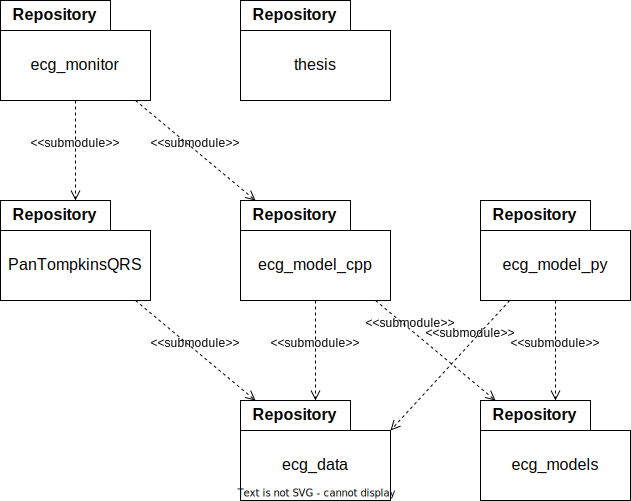
\includegraphics[width=\textwidth]{../assets/repositories.drawio}
    \bicaption{项目包含的Git仓库}{Git repositories of the project}
    \label{fig:repositories}
\end{figure}

\subsubsection{thesis}\label{subsubsec:repo-thesis}

这是本篇论文所在的仓库。论文本身作为项目文档的一部分,也被包含在本项目之中。该仓库包含论文的\LaTeX 源码,以及论文中引用的图片等资源文件,还有自动格式化、依赖版本管理、自动构建测试、自动发布新版本等持续集成配置。

论文与应用本身的代码是分离的,所以论文的仓库与应用的仓库之间没有任何子模块关系。此外,论文仓库以Git子树的形式包含了论文模板\footnote{\url{https://github.com/Koyamin/ECNUThesis-Undergraduate}},没有使用Git子模块是因为基于模板进行编写后只需要直接提交至主仓库,不需要向子仓库推送,这与~\ref{subsec:git-submodule} 节所述的情况不同。

\subsubsection{ecg\_monitor}\label{subsubsec:repo-monitor}

这是应用的主体仓库。该仓库包含基于Flutter框架编写的Dart代码,以及相关的各种配置文件等。仓库的命名与应用的包名一致,因此按照Dart对包名的相关限制使用了小写下划线的命名风格,而非Git仓库常用的小写连字符。为了保持项目各个仓库之间的一致性,其他仓库(除PanTompkinsQRS外)也都使用了小写下划线的命名风格。

为了方便调用C++代码,该仓库以Git子模块的形式包含了PanTompkinsQRS和ecg\_model\_cpp两个子仓库,这两个子仓库分别提供了Pan-Tompkins算法和基于LibTorch的心电图智能分析算法的实现。

\subsubsection{PanTompkinsQRS}\label{subsubsec:repo-qrs}

这是应用中用于实现Pan-Tompkins算法的仓库。该仓库是rafaelmmoreira编写的Pan-Tompkins算法的C语言实现\footnote{\url{https://github.com/rafaelmmoreira/PanTompkinsQRS}}的复刻(fork),在原始版本的基础上根据项目需要进行了一些修改。出于对原作者的尊重,该仓库的名称与原作者的命名保持一致,因此与项目内其他仓库的命名风格不同。

该仓库被ecg\_monitor所包含,并且为了方便测试而将ecg\_data包含为了子仓库,后者提供了一些测试用的心电图数据,用作测试时的输入。

\subsubsection{ecg\_model\_cpp}\label{subsubsec:repo-cpp}

这是应用中用于实现基于LibTorch的心电图智能分析算法的仓库。该仓库是ecg\_model\_py仓库的C++实现,使用了LibTorch作为框架。

该仓库被ecg\_monitor所包含,且包含了ecg\_data作为测试输入数据,还包含了ecg\_models作为与ecg\_model\_py共享的模型文件以及测试预期输出。

\subsubsection{ecg\_model\_py}\label{subsubsec:repo-py}

这是基于PyTorch实现的心电图智能分析算法的所在仓库。该仓库以算法的原始版本作为初始提交,在此基础上根据项目需要进行了修改。

Python版本的算法并不直接被应用调用,因此该仓库不是其他仓库的子模块。该仓库包含了ecg\_data作为测试输入数据,将与ecg\_model\_cpp共享的模型文件保存在ecg\_models,并将PyTorch版本的算法输出也写入ecg\_models子模块以便与ecg\_model\_cpp共享。

\subsubsection{ecg\_data}\label{subsubsec:repo-data}

该仓库存储了各算法仓库用作测试输入的心电图数据,以及从公开数据库下载心电数据并转换格式的相关代码。该仓库中的数据由仓库内的代码写入,被上述三个算法仓库所读取。

\subsubsection{ecg\_models}\label{subsubsec:repo-models}

该仓库存储了TorchScript模型文件,以及模型在测试输入下的输出结果。该仓库的内容由ecg\_model\_py写入,被ecg\_model\_cpp读取。因为模型文件较大(60多MB),且不被Pan-Tompkins算法所需要,所以该仓库与ecg\_data进行了分离。


\section{应用的界面与功能设计}\label{sec:app-design}

\subsection{应用的界面设计规范}\label{subsec:app-design-spec}

本应用与其他同类应用的一大差别在于其遵循专业的设计规范对应用界面进行了严格的设计。

应用整体上遵循Material 3设计规范\cite{MaterialDesign}。Material 3(也称为Material You)是Google在2021年5月的Google I/O大会上宣布的新一代Material设计规范,和前代规范相比具有从用户的壁纸自动生成动态主题颜色、按钮更大、界面动画更多等新特性,并在其他一些细节设计上有所优化。目前Material 3设计已被广泛应用于Google的各种应用程序,并成为Android应用的推荐设计规范。

尽管Material 3按照Google的设计是可以在任何平台(包括iOS)上使用的,但从事实上来说,iOS应用确实较少使用Material风格的设计,而较多按照苹果的推荐遵循Cupertino\footnote{苹果官方并未给自己的设计规范进行像Material这样的明确命名,Cupertino这个名字是Flutter在其文档中使用的,可能是基于苹果总部位于美国加利福尼亚州丘珀蒂诺(Cupertino)市的事实。}设计。为了符合iOS平台的用户习惯,本应用在iOS平台上将部分UI组件替换为了iOS应用常用的Cupertino风格的组件。由于Cupertino并未像Material一样提供全平台可用的设计,所以应用的设计仍然以Material为主,在Android平台上完全使用Material 3风格的设计,而在iOS平台上则使用Material 3风格与Cupertino风格的混合设计,如图~\ref{fig:android-ios} 所示。

\begin{figure}[ht]
    \subcaptionbox{Android}{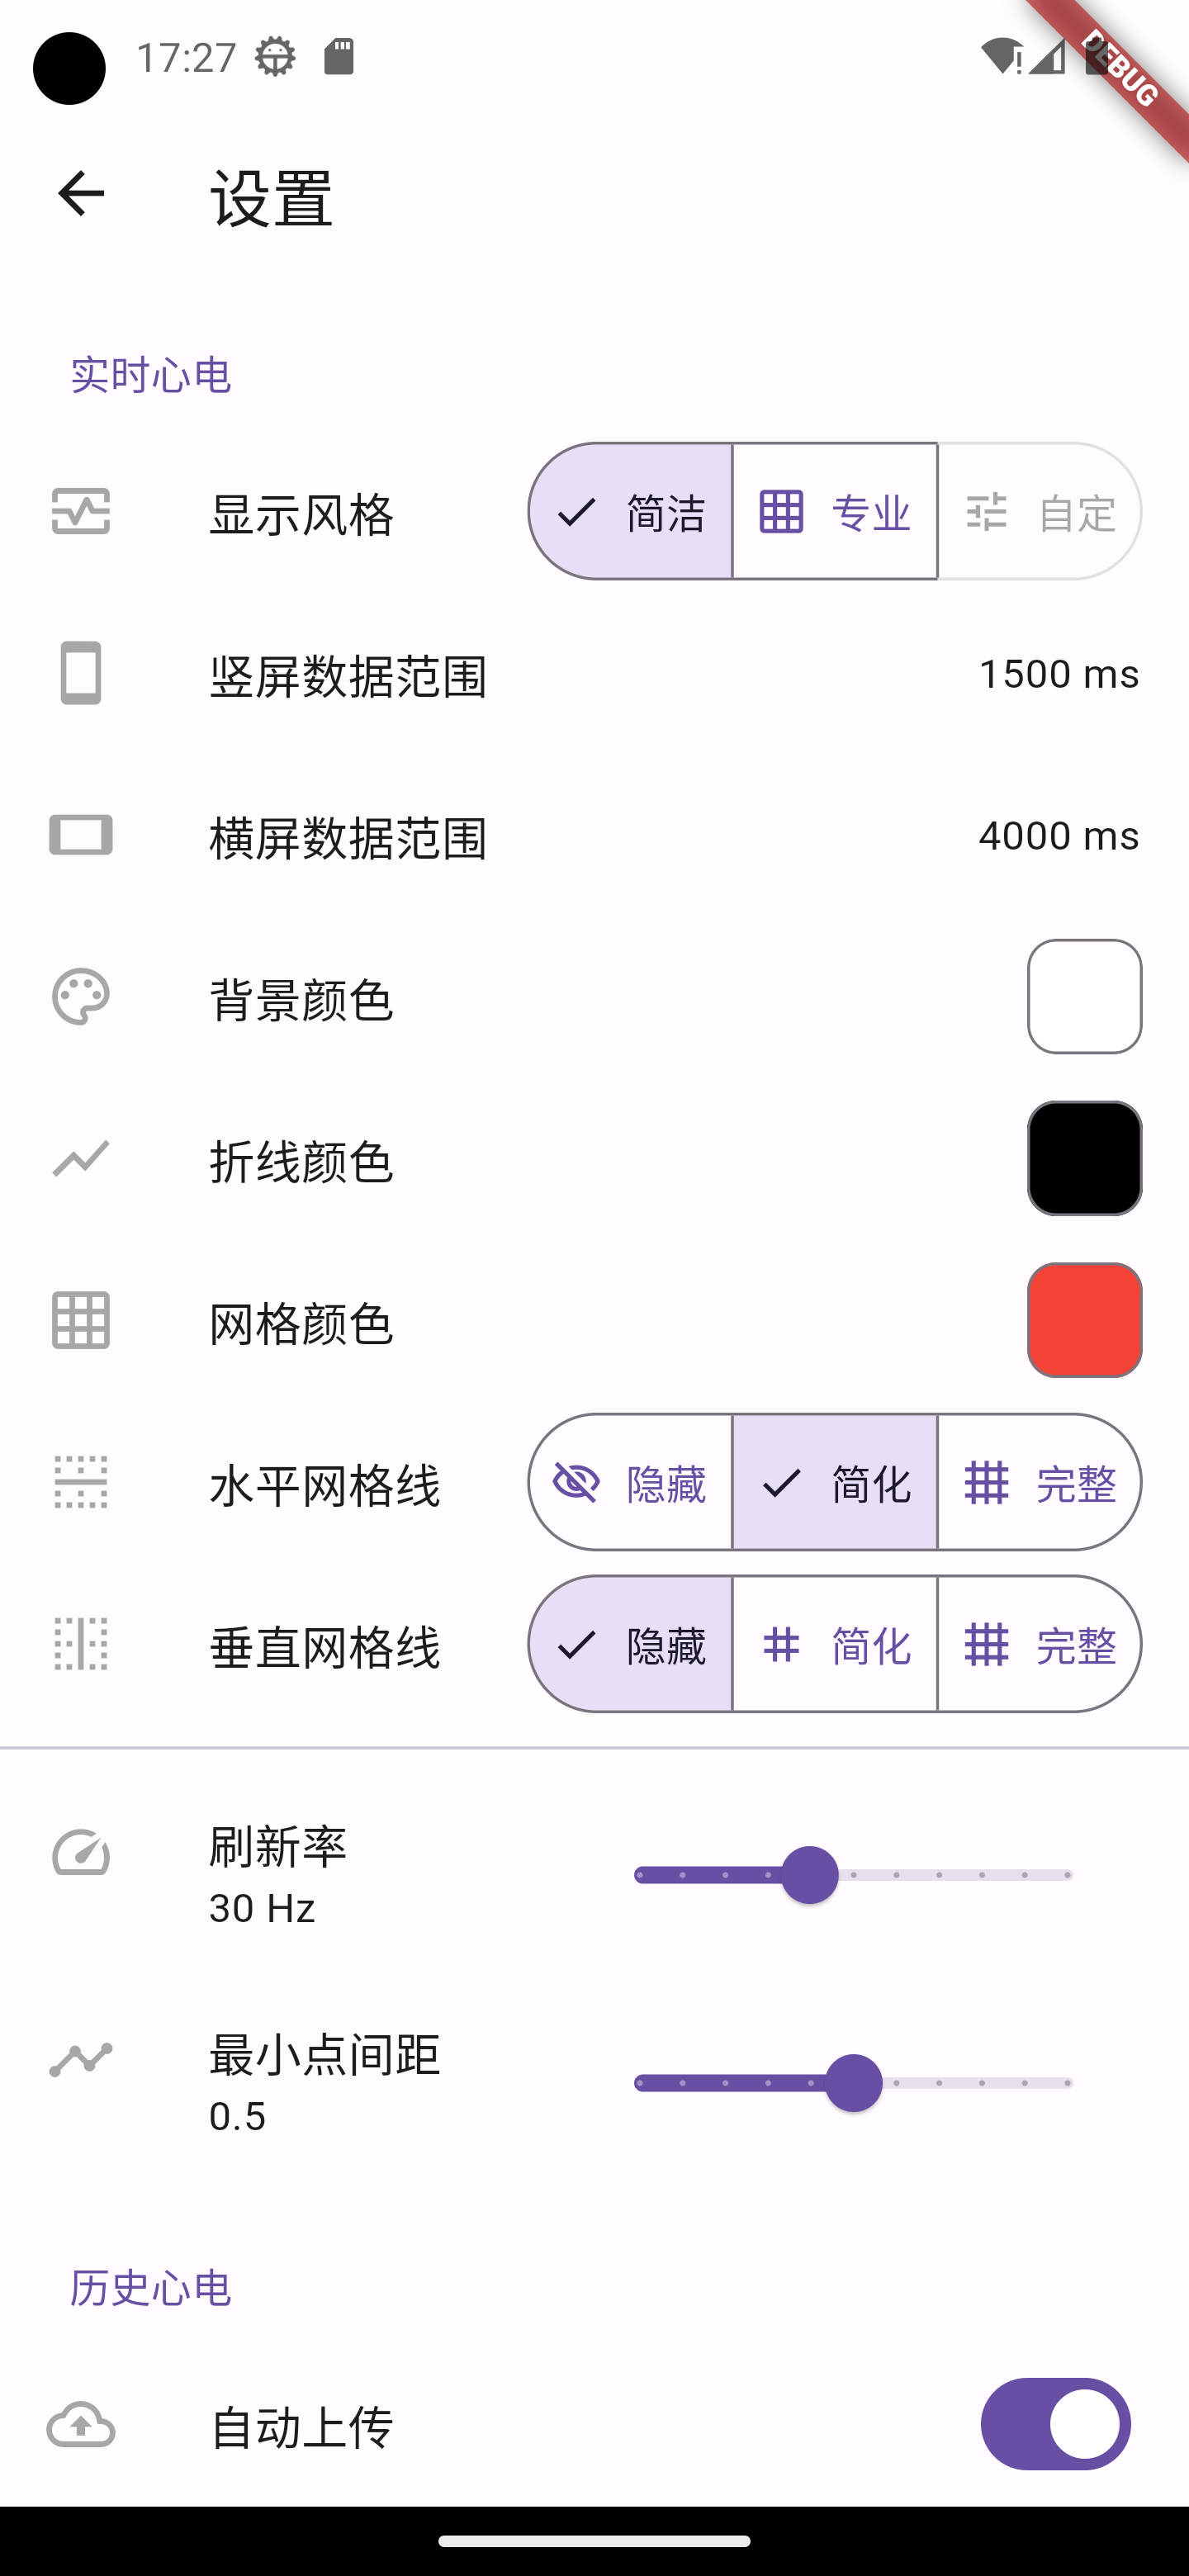
\includegraphics[height=17cm]{../assets/settings}}
    \subcaptionbox{iOS}{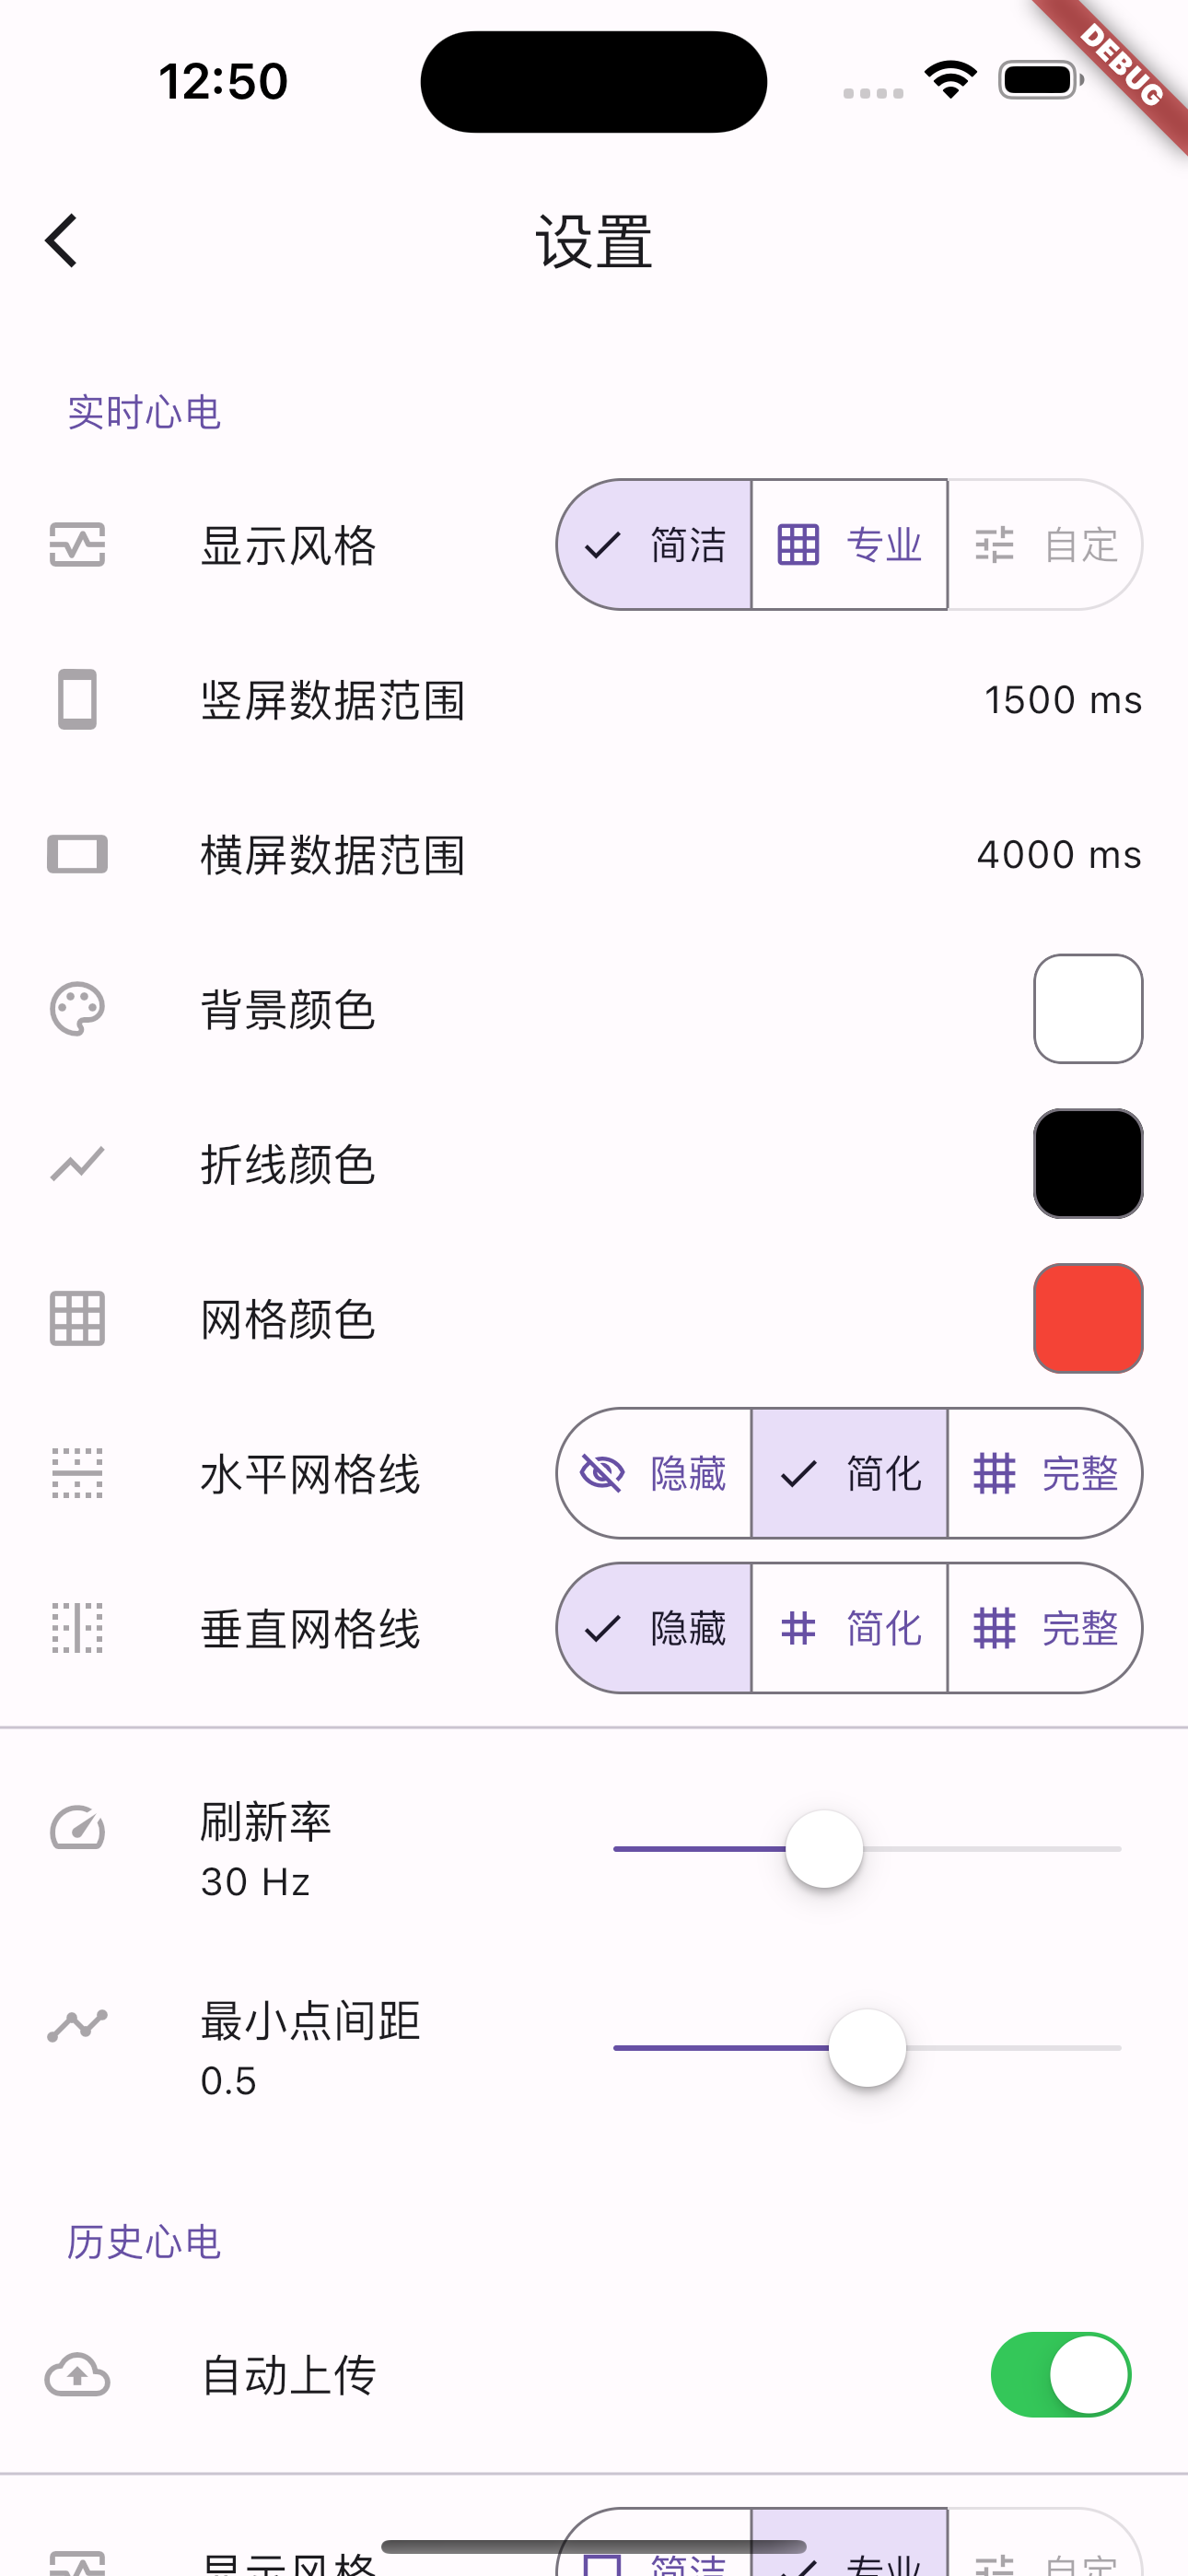
\includegraphics[height=17cm]{../assets/ios-settings}}
    \bicaption{应用在Android和iOS平台上的界面设计对比}{Comparison of the app's UI design on Android and iOS}
    \label{fig:android-ios}
\end{figure}

从图~\ref{fig:android-ios} 中可以看出应用在Android平台与iOS平台上的界面设计的一些差异,包括标题的对齐方式(Android居左,iOS居中)、左上角返回按钮的图标(Android使用完整箭头,iOS使用仅有头部的简化箭头)、滑动条与切换按钮的外观(按照各自规范中的相关要求)、文本的字体(iOS的字体更细)等。

\subsection{实时心电界面的设计}\label{subsec:real-time-design}

实时心电界面的整体设计如图~\ref{fig:real-time} 所示。

\begin{figure}[ht]
    \subcaptionbox{心率检测中}{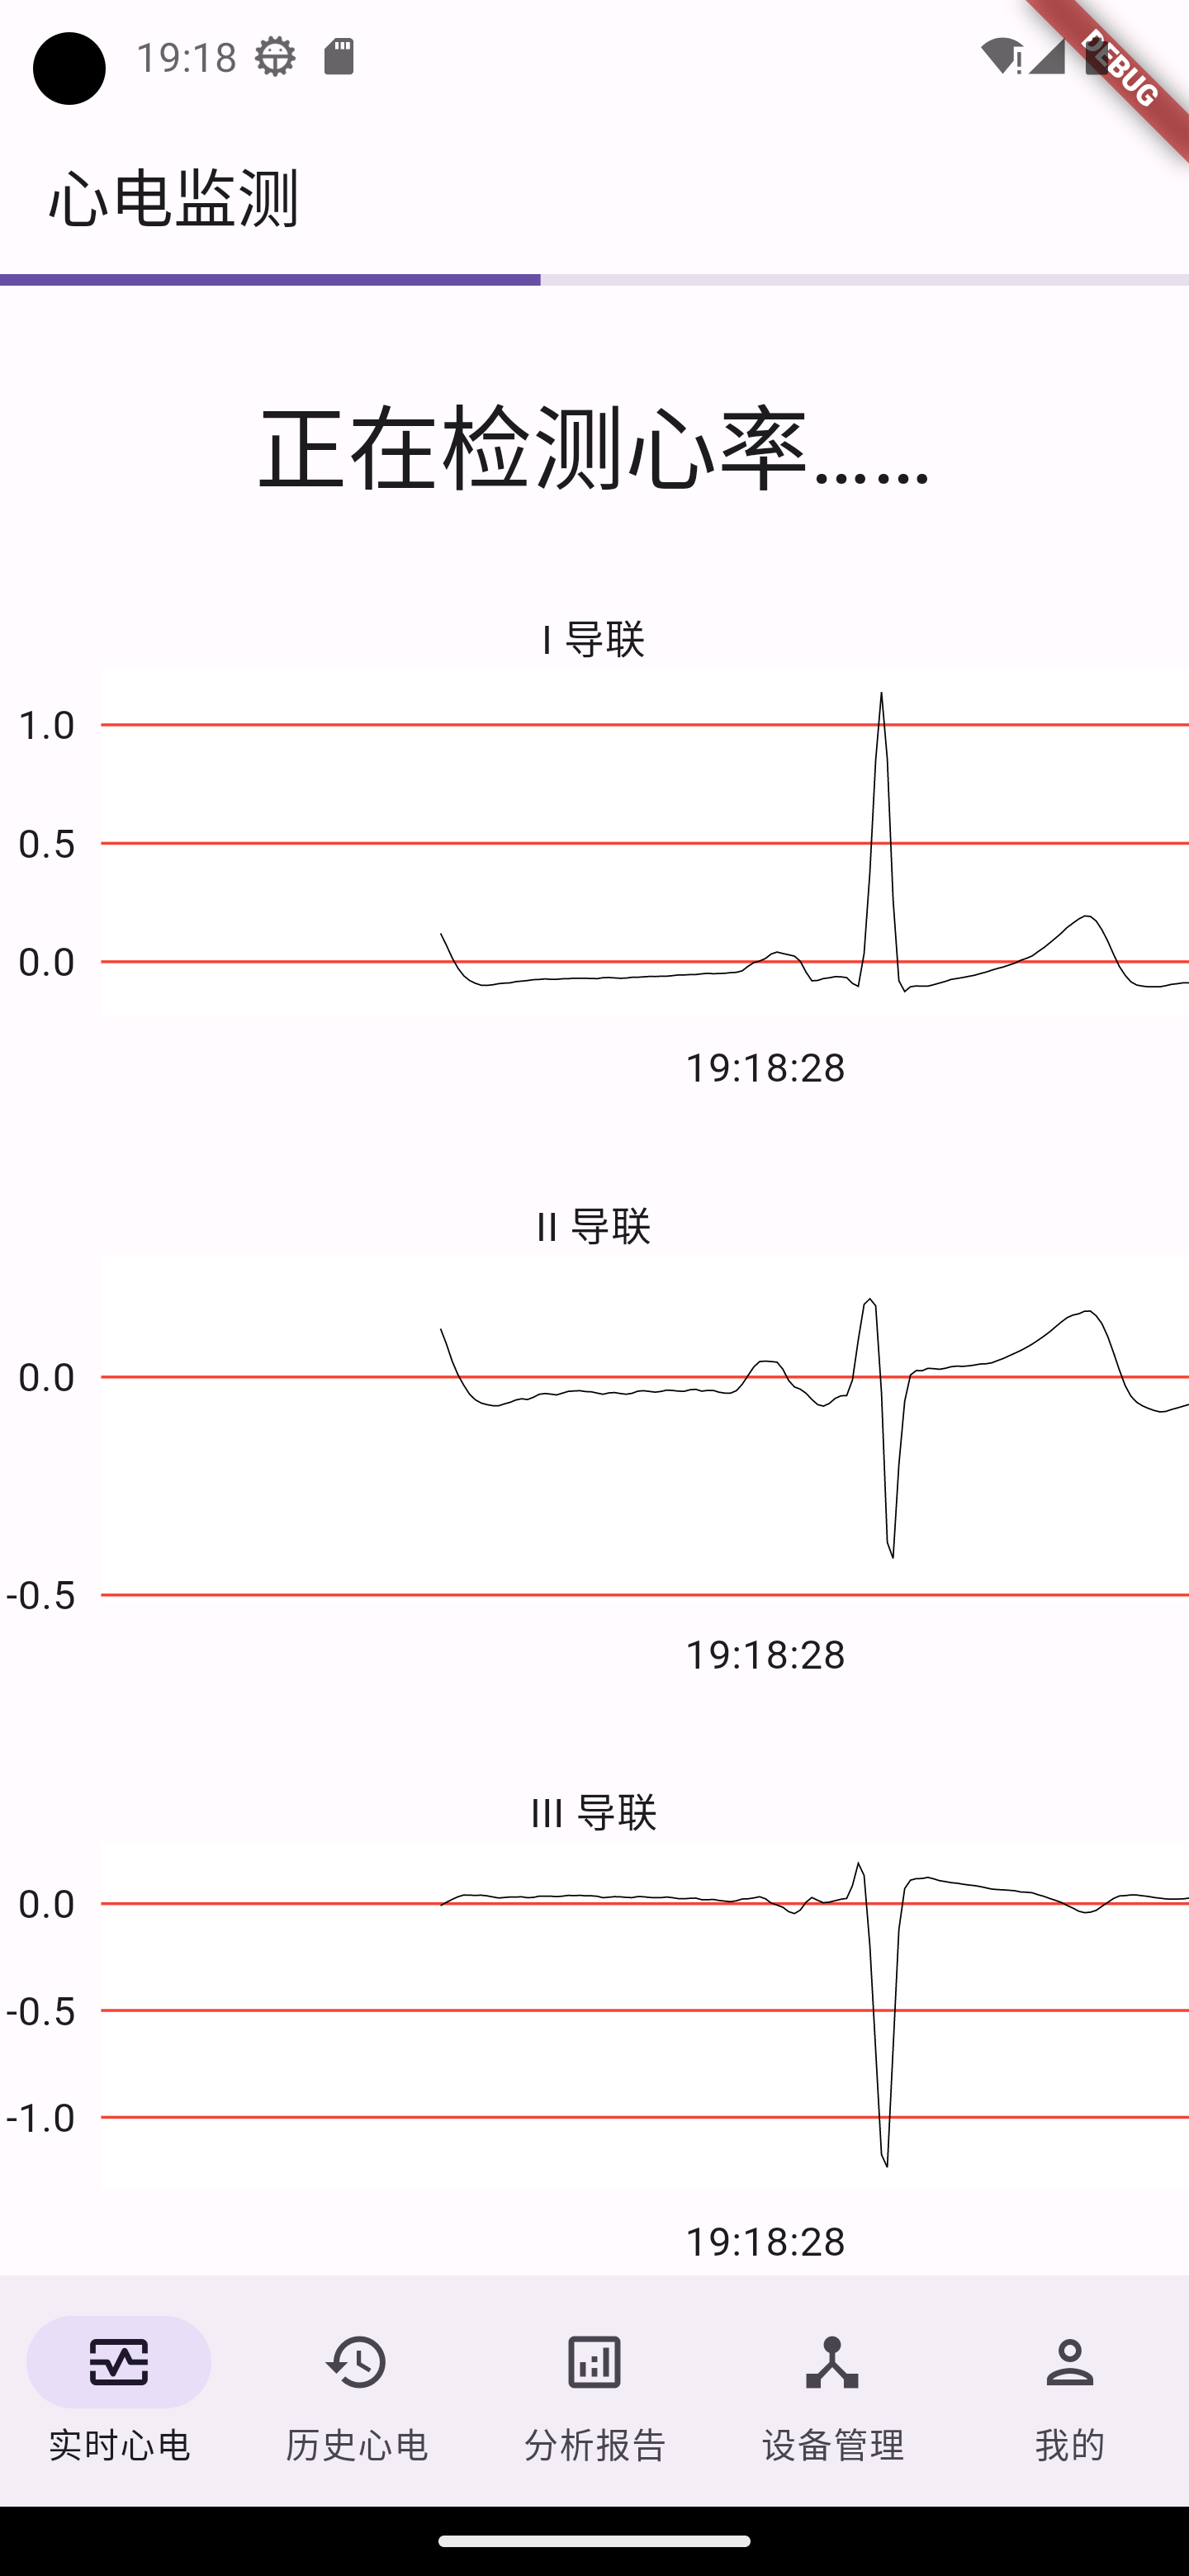
\includegraphics[width=.33\textwidth]{../assets/real-time-learning}}
    \subcaptionbox{正常状态}{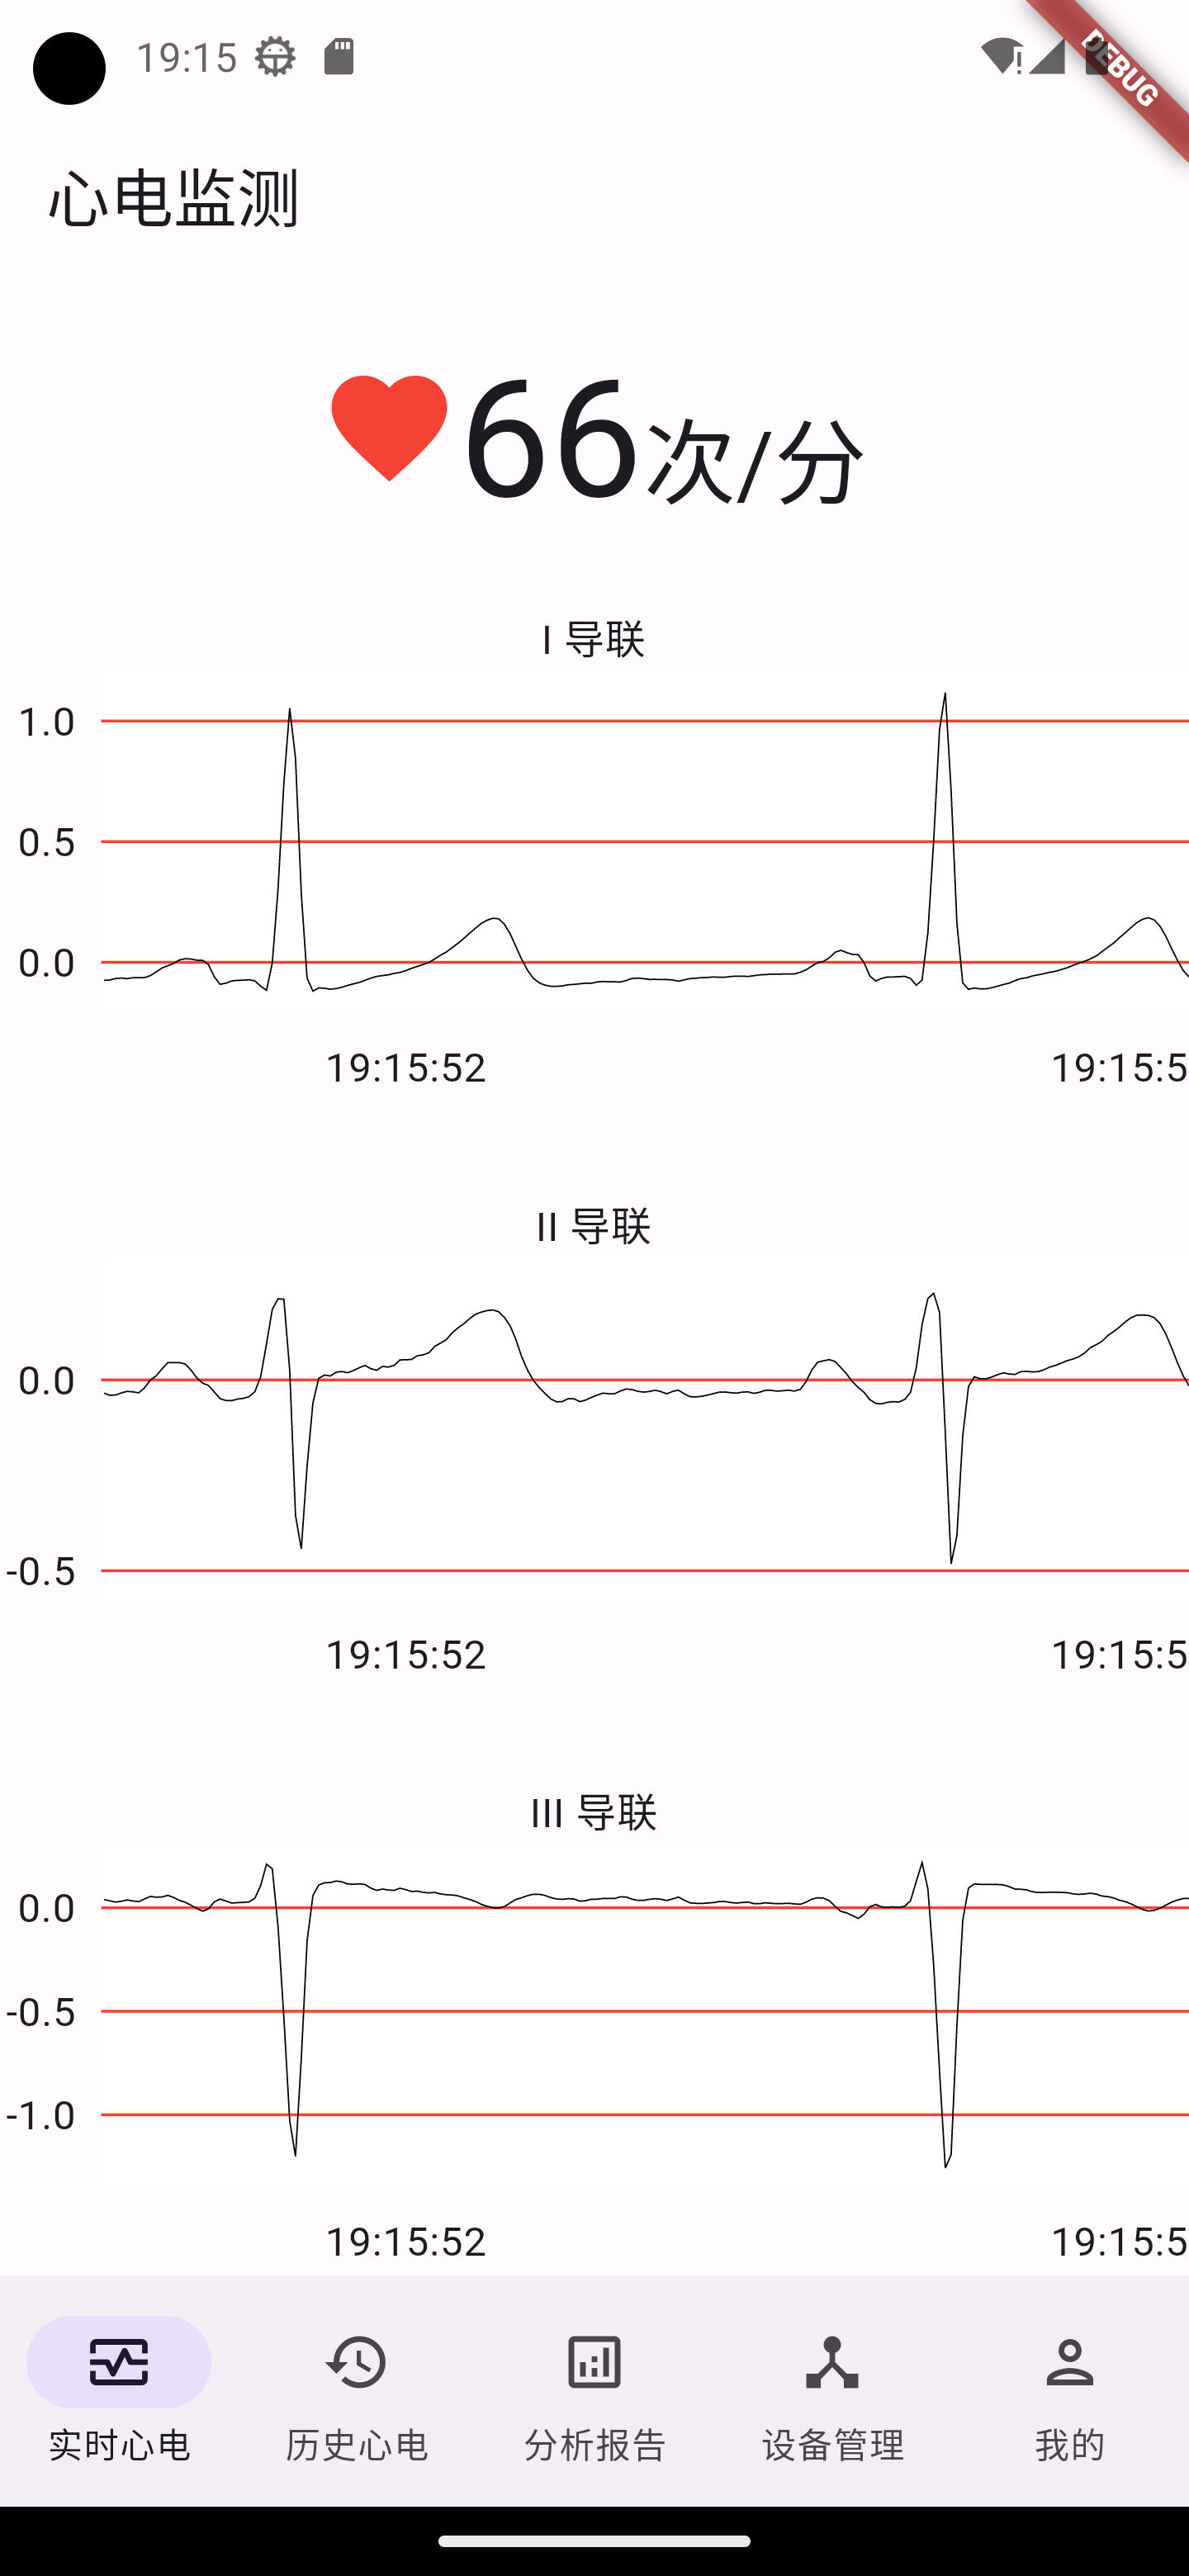
\includegraphics[width=.33\textwidth]{../assets/real-time}}
    \subcaptionbox{设备未连接}{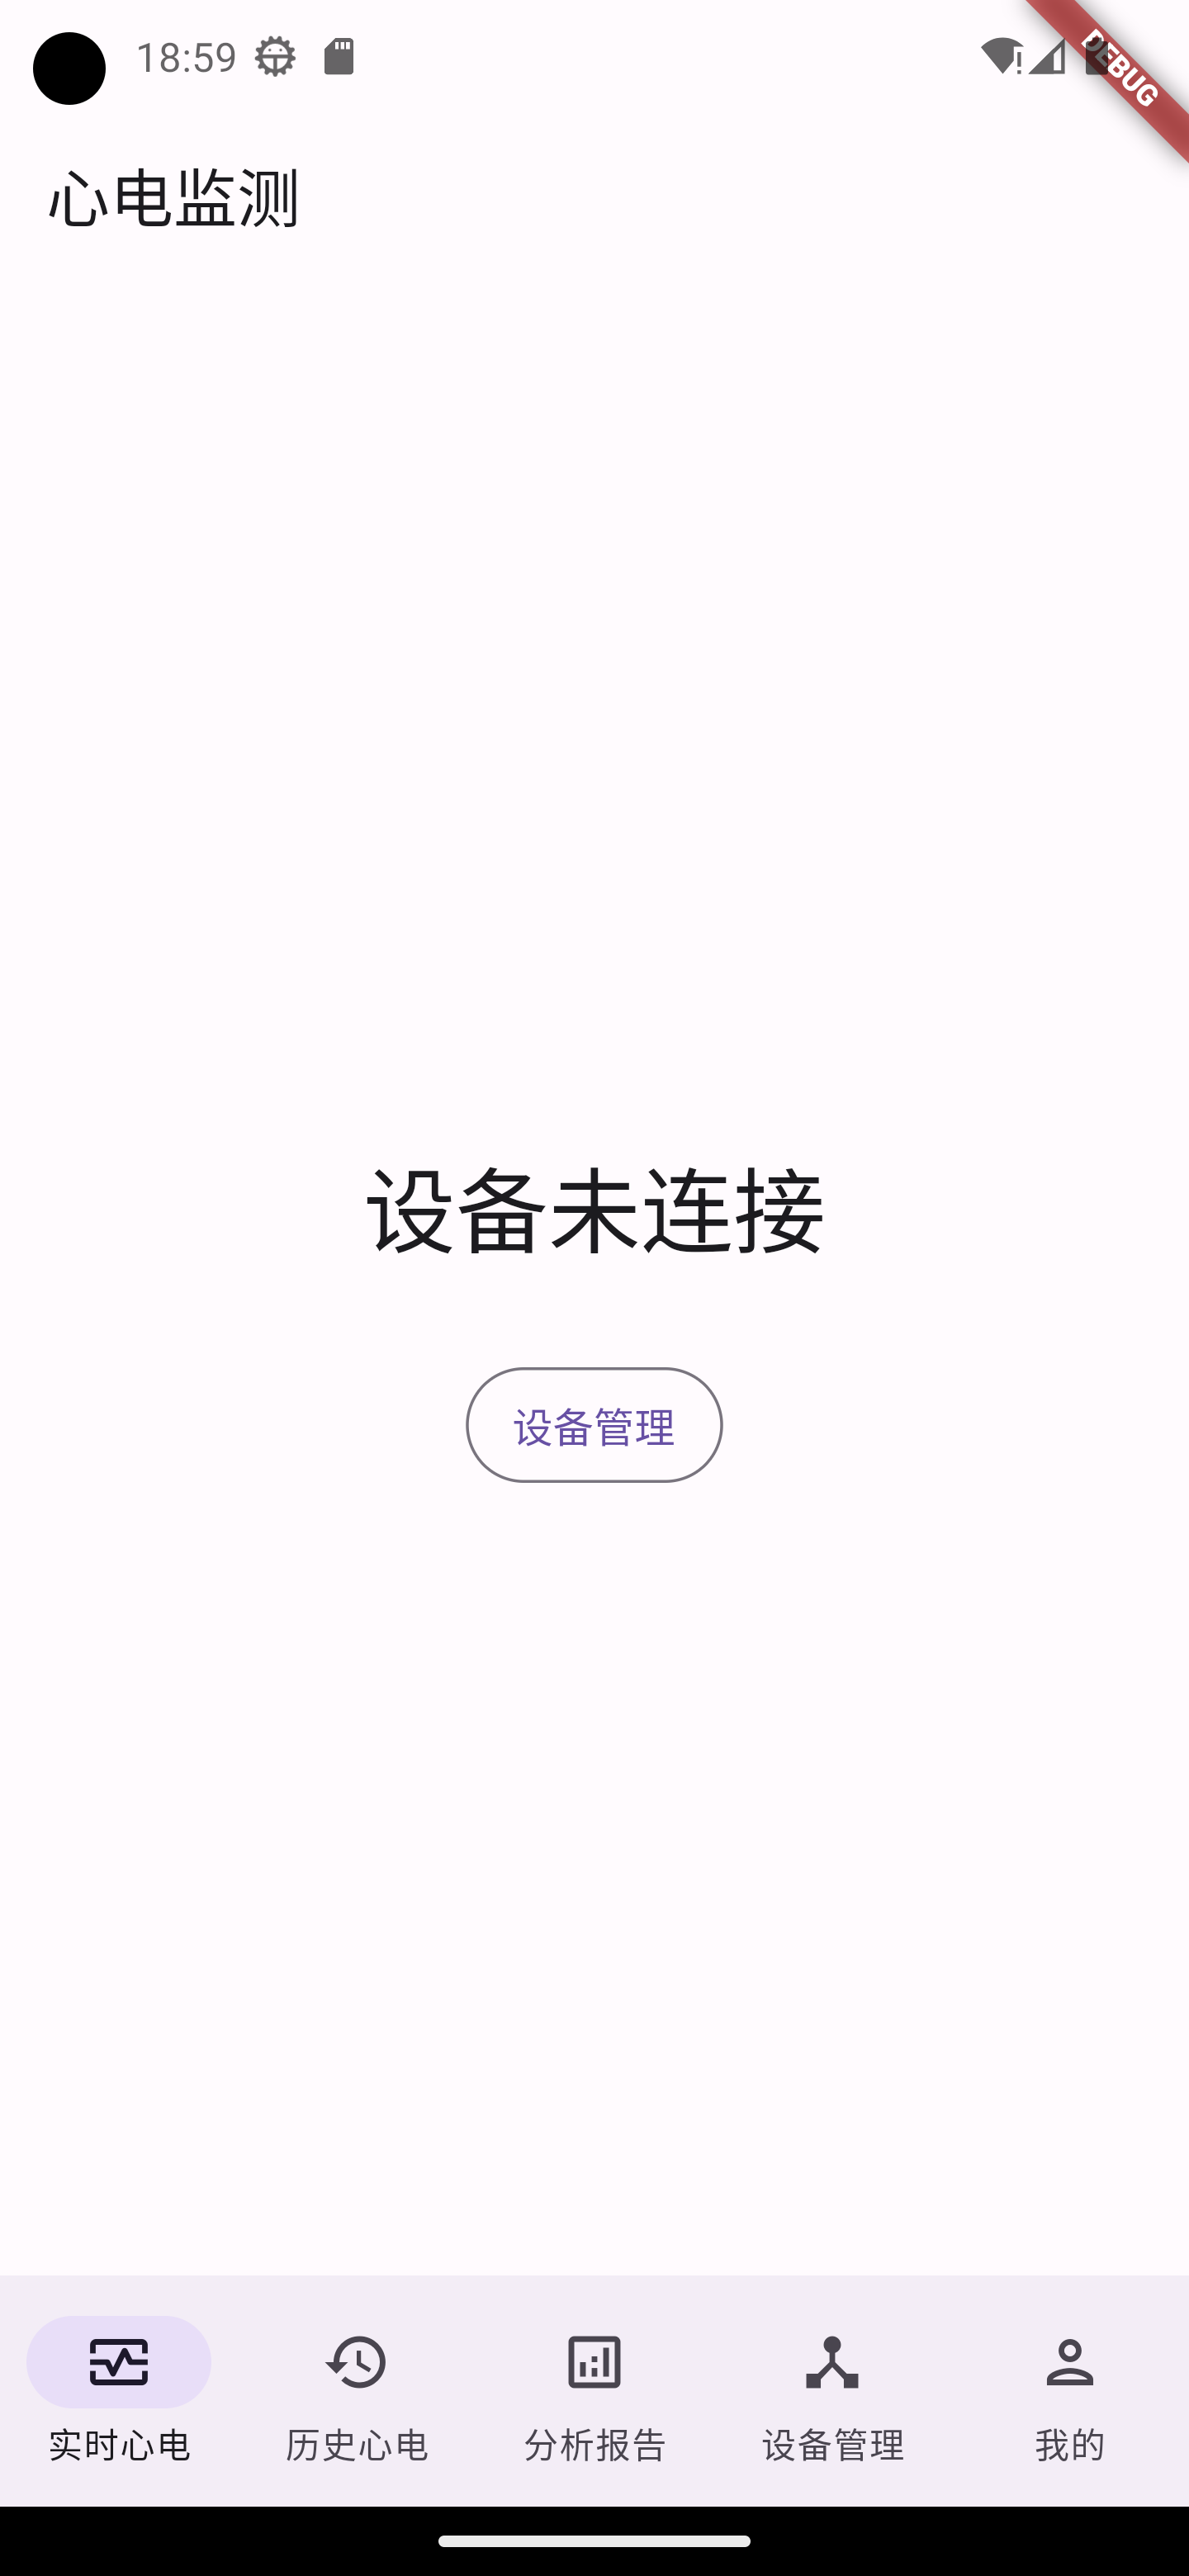
\includegraphics[width=.33\textwidth]{../assets/real-time-na}}
    \bicaption{实时心电界面的设计}{Design of the real-time ECG page}
    \label{fig:real-time}
\end{figure}

实时心电界面的主体可以分为心率和心电图两大部分。另外,在整个应用的最上方显示了应用的名称,最下方显示了应用的导航栏,导航栏提供了应用中最主要的几个界面的入口。

\subsubsection{心率部分的设计}\label{subsubsec:heart-rate-design}

实时心电界面的上方显示了用户当前的心率。

当用户刚刚佩戴上或连接上心电监测设备的时候,由于缺少数据,心率无法立即获得。在这种状态下,心率部分会显示“正在检测心率……”作为占位符,并且上方会显示一个线状的进度条。Material规范中规定了两种类型的线状进度条,分别表示确定的和不确定的进度。因为心率检测所需的时间可以大致确定,所以此处使用了确定进度的版本,进度条的已填充长度占比表示心率检测的预测进度。进度条的使用可以向用户提供检测进度的视觉反馈,虽然并不能在实际上加快检测速度,但由于减少了不确定性,仍然可以减少用户在等待过程中的焦虑感与沮丧感,起到了与加快检测速度类似的作用。反之,如果在系统正在工作的过程中不为用户提供指示,比如大夏学堂在上传作业文件时的设计,即使是在只需要等待数秒的情况下,用户也会感到焦虑与沮丧,在更长时间后甚至会由于缺乏对任务最终可以完成的信心而感到挫折并放弃使用。进度条虽然只是个简单的组件,但对于软件的易用性和用户体验来说却是个关键设计。

心率检测的结果可用之后,该区域则会显示心率数据。显示内容由横向排布的三个组件组成:图标、数值和单位。图标使用了一个红色的心形标志,主要起到两个作用:一是指示该区域显示的内容是心率,由于应用的性质与该界面其他元素的暗示,用户很容易理解到所示数值表示心率,所以不需要使用文本等方式进行明确说明,只使用简单的图标已经足够;二是加强该区域的视觉强调效果,由于心率区域在整个屏幕上的面积占比较少,但重要性并不显著弱于下方的心电图等元素,所以使用了这个颜色较为鲜艳的图标来将用户的注意力吸引至该区域。数值和单位使用了不同大小的字体,数值较大而单位较小。这是因为心率数值是该区域的主要内容,且不断变动,需要较为强调。而心率的单位是固定的,不会变动,而且每分钟的次数(bpm)作为最常用的心率单位已经为用户所习惯,不需要特别强调,所以使用较小的字体弱化了单位的视觉效果,以突出其他部分。三个组件在横向与纵向上整体居中,内部按文本基线对齐(即靠下对齐)。

此外,整个心率显示区域在实时心电界面上的高度占比是固定的,以免在检测完成前后以及数值变动时引起下方心电图位置的上下移动。

\subsubsection{心电图部分的设计}\label{subsubsec:ecg-design}

心电图部分的设计参考了医学上常用的心电图纸的设计。心电图纸的整体外观在\nameref{ch:intro}部分的图~\ref{fig:10sec-ekg-lead} 中已经展示过,这里对其具体布局方式进行一些补充介绍。

心电图纸包含红色的坐标线,如图~\ref{fig:ecg-paper} 所示。每1mm一小格(用细线分隔),每5mm一大格(用粗线分隔)。横轴一小格表示40ms,一大格表示200ms。纵轴一小格表示0.1mV,一大格表示0.5mV。心电图纸的左侧有1mV(10mm高)的参考波形,并标注该条图像的导联名称。

\begin{figure}[ht]
    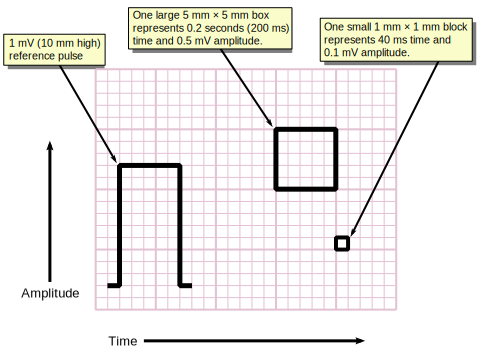
\includegraphics[width=\textwidth]{../assets/ECG_Paper_v2}
    \bicaption{心电图纸的布局}{Layout of ECG paper}
    \label{fig:ecg-paper}
\end{figure}

在应用内实时心电图的设计过程中,对心电图纸的元素进行了一些精简与修改。首先,由于移动设备的屏幕尺寸较小,将心电数据的显示范围进行了缩减,纵轴范围根据当前图中显示的心电数据自适应变动,以最大值加0.1mV作为上限,最小值减0.1mV作为下限。横轴范围则按照心电数据的常见电压范围进行了等比例调整,使其与纵轴比例可以保持近似对应,并在应用设置内增加了相关的选项供用户按需自行调整。之后,由于纵向坐标线在实时心电图的快速移动的过程中会产生视觉上的严重干扰,所以将其去除,改为在下方显示数据对应的时间;为了保持视觉上的协调,横轴坐标线去除了划分小格的细线,仅保留了0.5mV一条的粗线。最后,考虑到一般用户对心电图纸的参考波形的了解程度较低,加之移动设备的显示空间有限,所以将参考波形去除,改为在左侧显示电压数值,并相应地将导联名称移至心电图的正上方中央。

心电图部分在竖屏和横屏状态下有不同的显示方式。竖屏状态下,如之前所示,三个导联的心电图从上到下竖向排布在该区域。由于移动设备的屏幕宽度较窄,所以竖屏状态下可以显示的时长也较短,屏幕中每个导联通常只能显示一到两个心拍。虽然可以在应用设置中对显示时长进行调整,但在显示区域的宽度无法改变的情况下,显示更长时间的数据只能是以降低细节的可见程度为代价的。为了提供一种可以在不提高显示密度的情况下查看更长时间的数据的方式,应用在横屏状态下会改为仅显示单个导联的数据,如图~\ref{fig:real-time-landscape} 所示。

\begin{figure}[ht]
    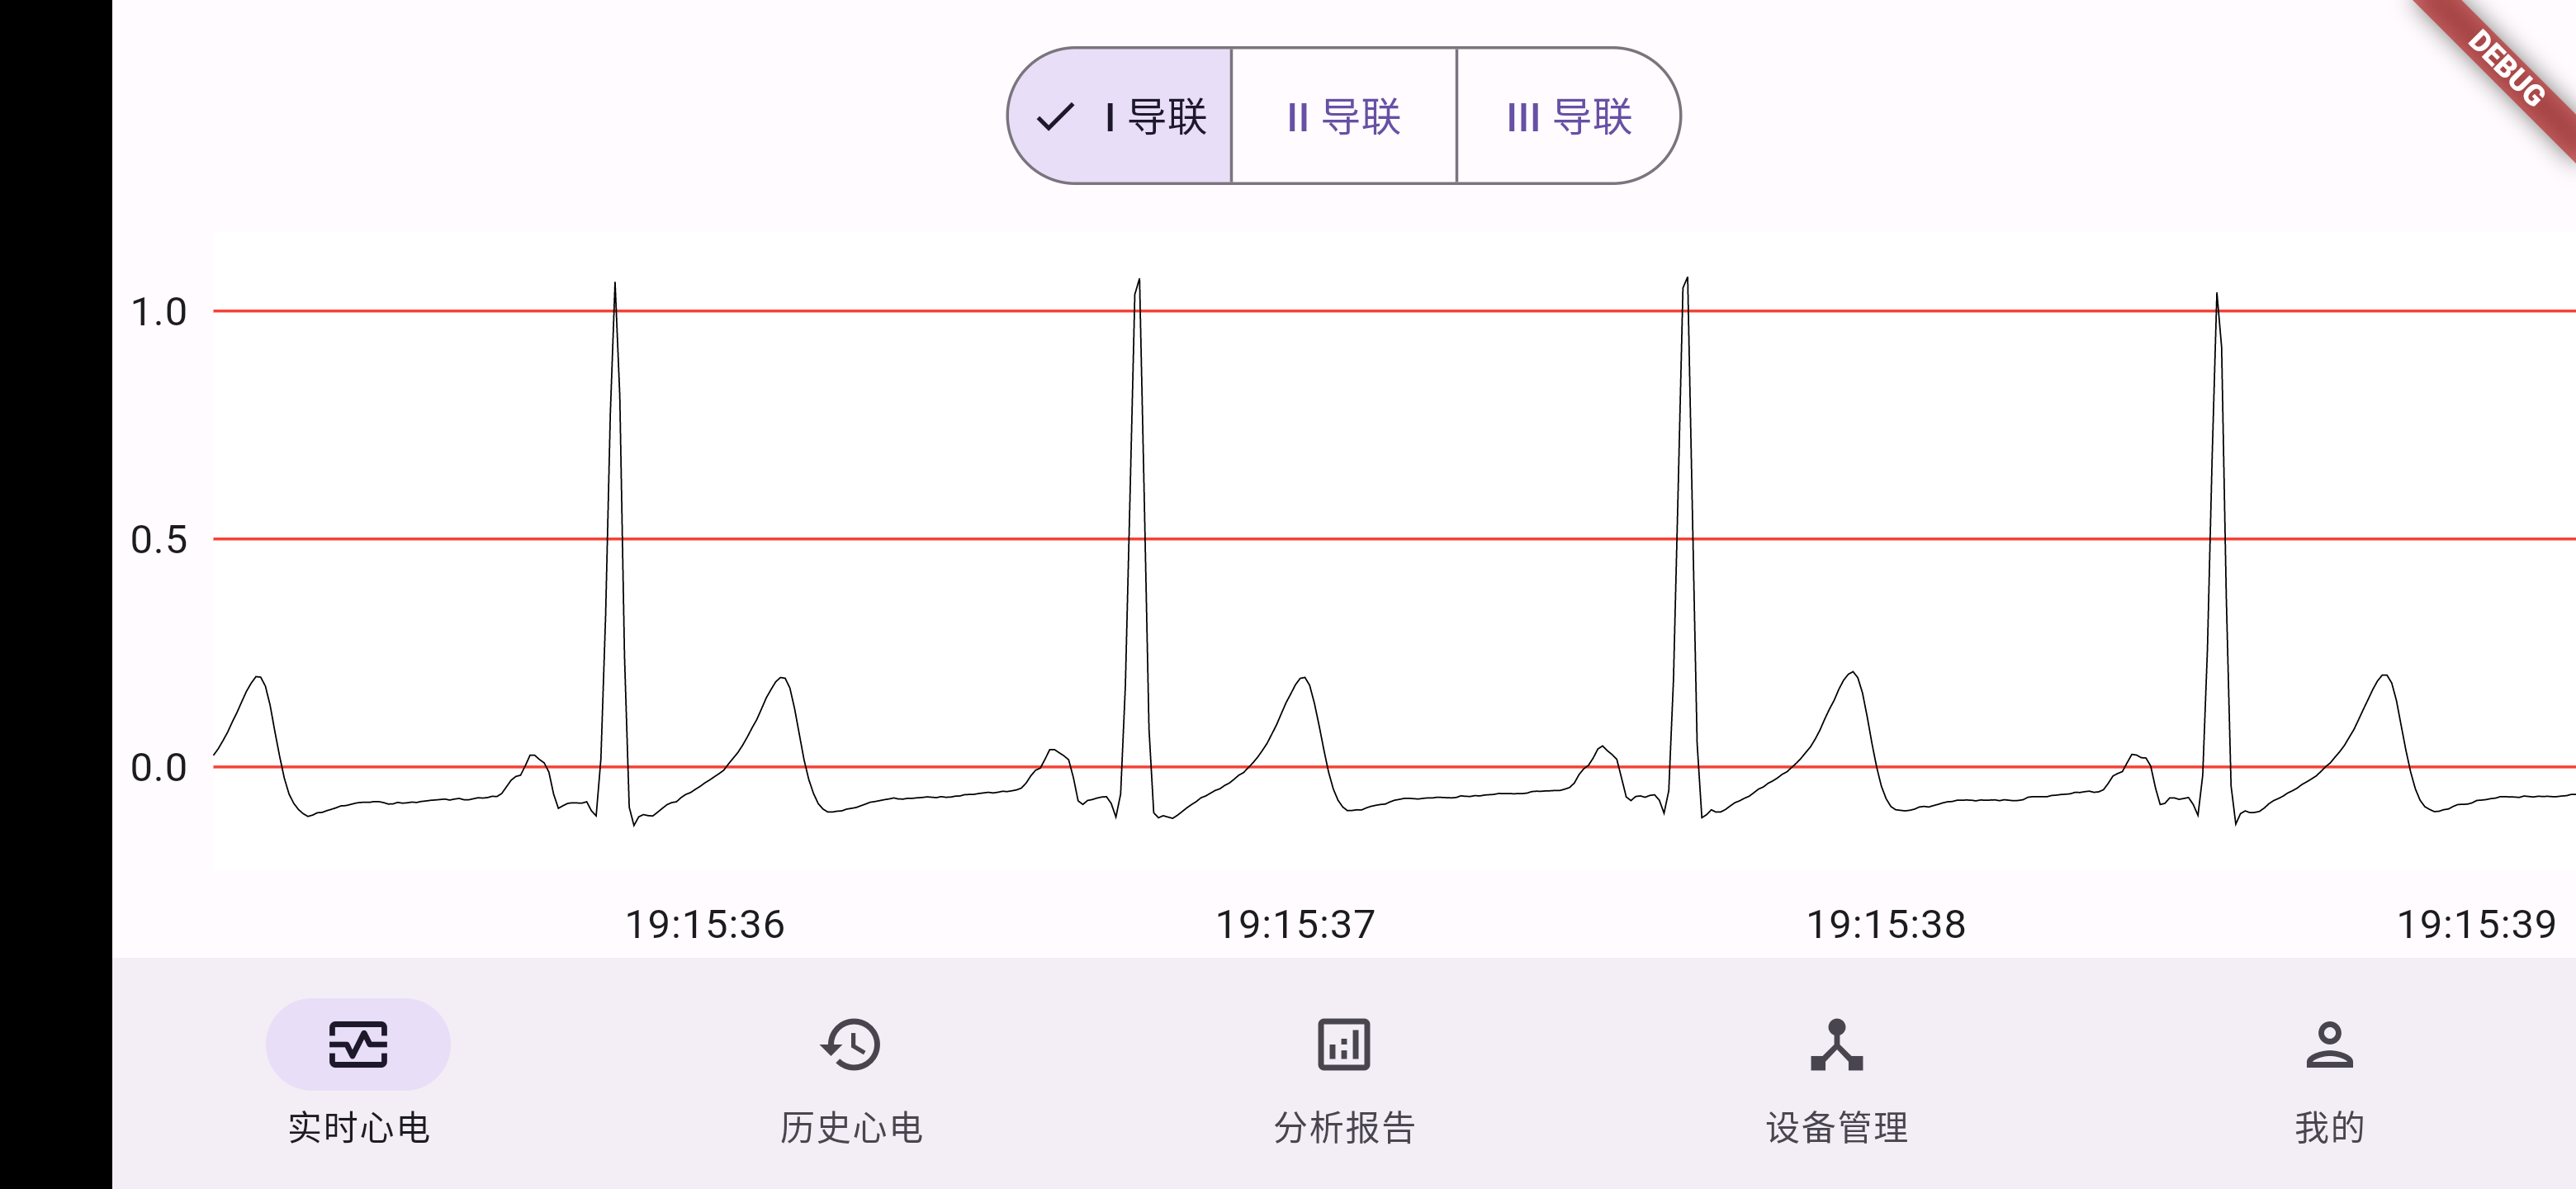
\includegraphics[width=\textwidth]{../assets/real-time-landscape}
    \bicaption{横屏状态下的心电图设计}{Design of the ECG in landscape mode}
    \label{fig:real-time-landscape}
\end{figure}

在横屏状态下,应用会进入全屏状态,隐去系统自带的状态栏等元素。在应用界面内部,顶端的标题栏以及屏幕上部的心率显示区域也会隐藏,以提供更多纵向空间。心电图区域会由同时显示三个导联变为仅显示单个导联,并将心电图上方的导联名称替换为分段按钮,以便用户可以在不同的导联之间进行切换。在横屏状态下,应用在心电图之外仍然为上方的导联切换按钮与下方的导航栏保留了足够的空间。这一方面是因为Material规范要求可点击的元素必须保留足够的大小,以便用户可以轻松点击;另一方面是因为如果要让心电图在保持横纵比例不变的情况下显示更长的时间,纵向空间就需要进行相应缩减;同时,这也保证了在横屏状态下仍然可以正常使用应用的基本功能,使用户不需要在进行切换界面等操作之前先将设备恢复为竖屏状态。

\subsubsection{设备未连接状态的设计}\label{subsubsec:real-time-na-design}

在设备未连接的情况下,由于无从获取实时心电数据,实时心电界面没有可供查看的实际内容。如果仅显示没有数据的空心电图,可能会使用户产生疑惑。因此,在设备未连接的情况下,应用会将实时心电界面替换为一个特殊的错误提示界面。该界面非常简洁,仅在显示区域的中央包含两个元素,竖向排布并留有一定间隔。上方以较大字体显示“设备未连接”的提示信息,下方以按钮形式提供前往设备管理界面的入口,提醒用户检查设备的状态。由于用户可能会在应用保持处于该界面的情况下调试心电设备,所以即使在心电设备尚未连接的情况下,应用也不会自动重定向至设备管理页,而是在用户手动点击按钮后才会跳转。

Material设计提供了各种风格的按钮外观设计。在该提示界面中,比较适用的几种风格如图~\ref{fig:buttons} 所示。

\begin{figure}[ht]
    \subcaptionbox{抬升按钮}{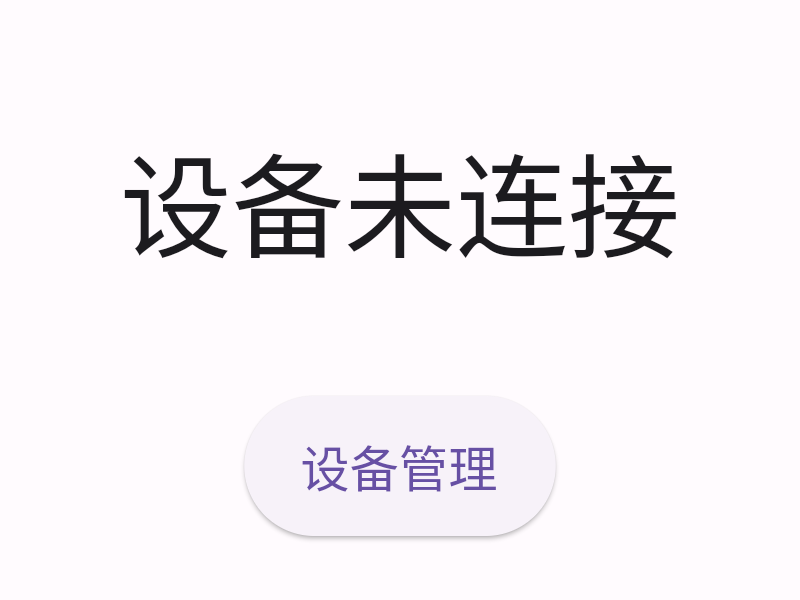
\includegraphics[width=.196\textwidth]{../assets/button-elevated}}
    \subcaptionbox{填充按钮}{
\includegraphics[width=.196\textwidth]{../assets/button-filled}}
    \subcaptionbox{填充色调按钮}{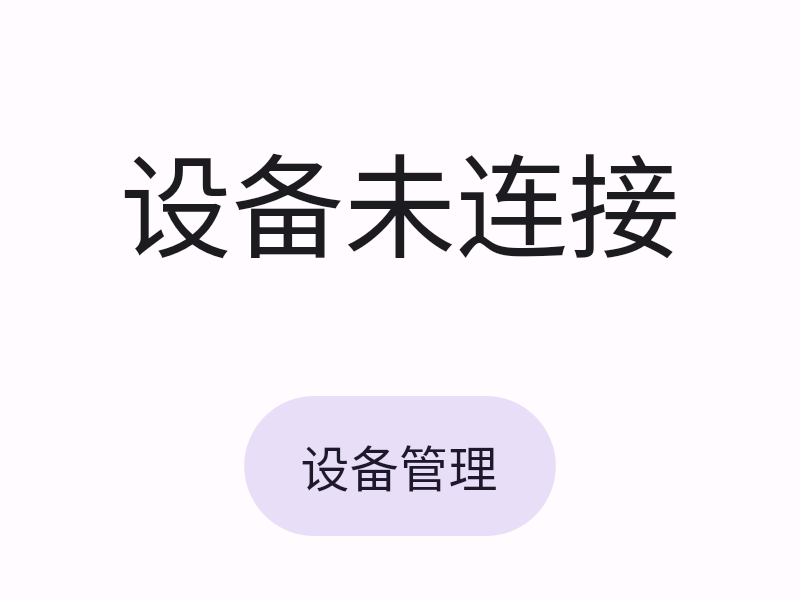
\includegraphics[width=.196\textwidth]{../assets/button-filled-tonal}}
    \subcaptionbox{轮廓按钮}{
\includegraphics[width=.196\textwidth]{../assets/button-outlined}}
    \subcaptionbox{文本按钮}{
\includegraphics[width=.196\textwidth]{../assets/button-text}}
    \bicaption{各种风格的按钮对比}{Comparison of different button styles}
    \label{fig:buttons}
\end{figure}

图中从左到右分别为抬升按钮(Elevated button)、填充按钮(Filled button)、填充色调按钮(Filled tonal button)、轮廓按钮(Outlined button)和文本按钮(Text button)。其中,抬升按钮因其阴影效果较易与其他元素之间产生不协调感,被规定为仅在绝对必要的时候,比如需要从图案背景中进行视觉分离时等特殊情况下才应使用,显然此界面并不属于应添加阴影的特殊情况。其余四种按钮的强调程度由强至弱,应当按需使用。由于该界面元素较少,所以不需要对该按钮进行较为强烈的强调,故未使用两种填充按钮。如果使用文本按钮,则视觉效果过于微弱,甚至使用户有些难以察觉到这是一个按钮。最终,选定了轮廓按钮的风格,其强调程度充足但不过度,与其他元素最为协调。

\subsubsection{应用中图标的设计}\label{subsubsec:icons}

实时心电界面在导航栏中的图标使用了常见的心电图的标志,这是根据该界面的主要内容决定的。

Material规范对于图标的设计与使用有一些相关要求。本应用为了遵循规范,使用的均是Google官方提供的图标。Google为其图标提供了各种风格的样式,常见的几种如图~\ref{fig:icons} 所示。

\begin{figure}[ht]
    \centering
    \subcaptionbox{轮廓}{
\includegraphics[width=.15\textwidth]{../assets/icon-outlined}}
    \subcaptionbox{圆润}{
\includegraphics[width=.15\textwidth]{../assets/icon-rounded}}
    \subcaptionbox{尖锐}{
\includegraphics[width=.15\textwidth]{../assets/icon-sharp}}
    \subcaptionbox{常规(旧)}{
\includegraphics[width=.15\textwidth]{../assets/icon-old-outlined}}
    \subcaptionbox{填充(旧)}{
\includegraphics[width=.15\textwidth]{../assets/icon-old-filled}}
    \bicaption{Material图标的各种风格}{Different styles of Material icons}
    \label{fig:icons}
\end{figure}

图中的前三种风格是Material 3新增的,通常应该比旧版优先使用。具体使用哪一种风格应该根据应用程序的整体设计风格来确定,比如圆润的图标使用了较多圆角,与使用较重的排版、弯曲徽标或圆形元素来表达其风格的品牌搭配得很好;尖锐的图标则带有较多直角,体现出清晰锐利的风格。本应用内的所有图标都使用了轮廓风格,这和整个应用的轻盈、干净的设计风格保持一致。

\subsection{历史心电界面的设计}\label{subsec:history-design}

历史心电界面的整体设计如图~\ref{fig:history} 所示。

\begin{figure}[ht]
    \subcaptionbox{加载中}{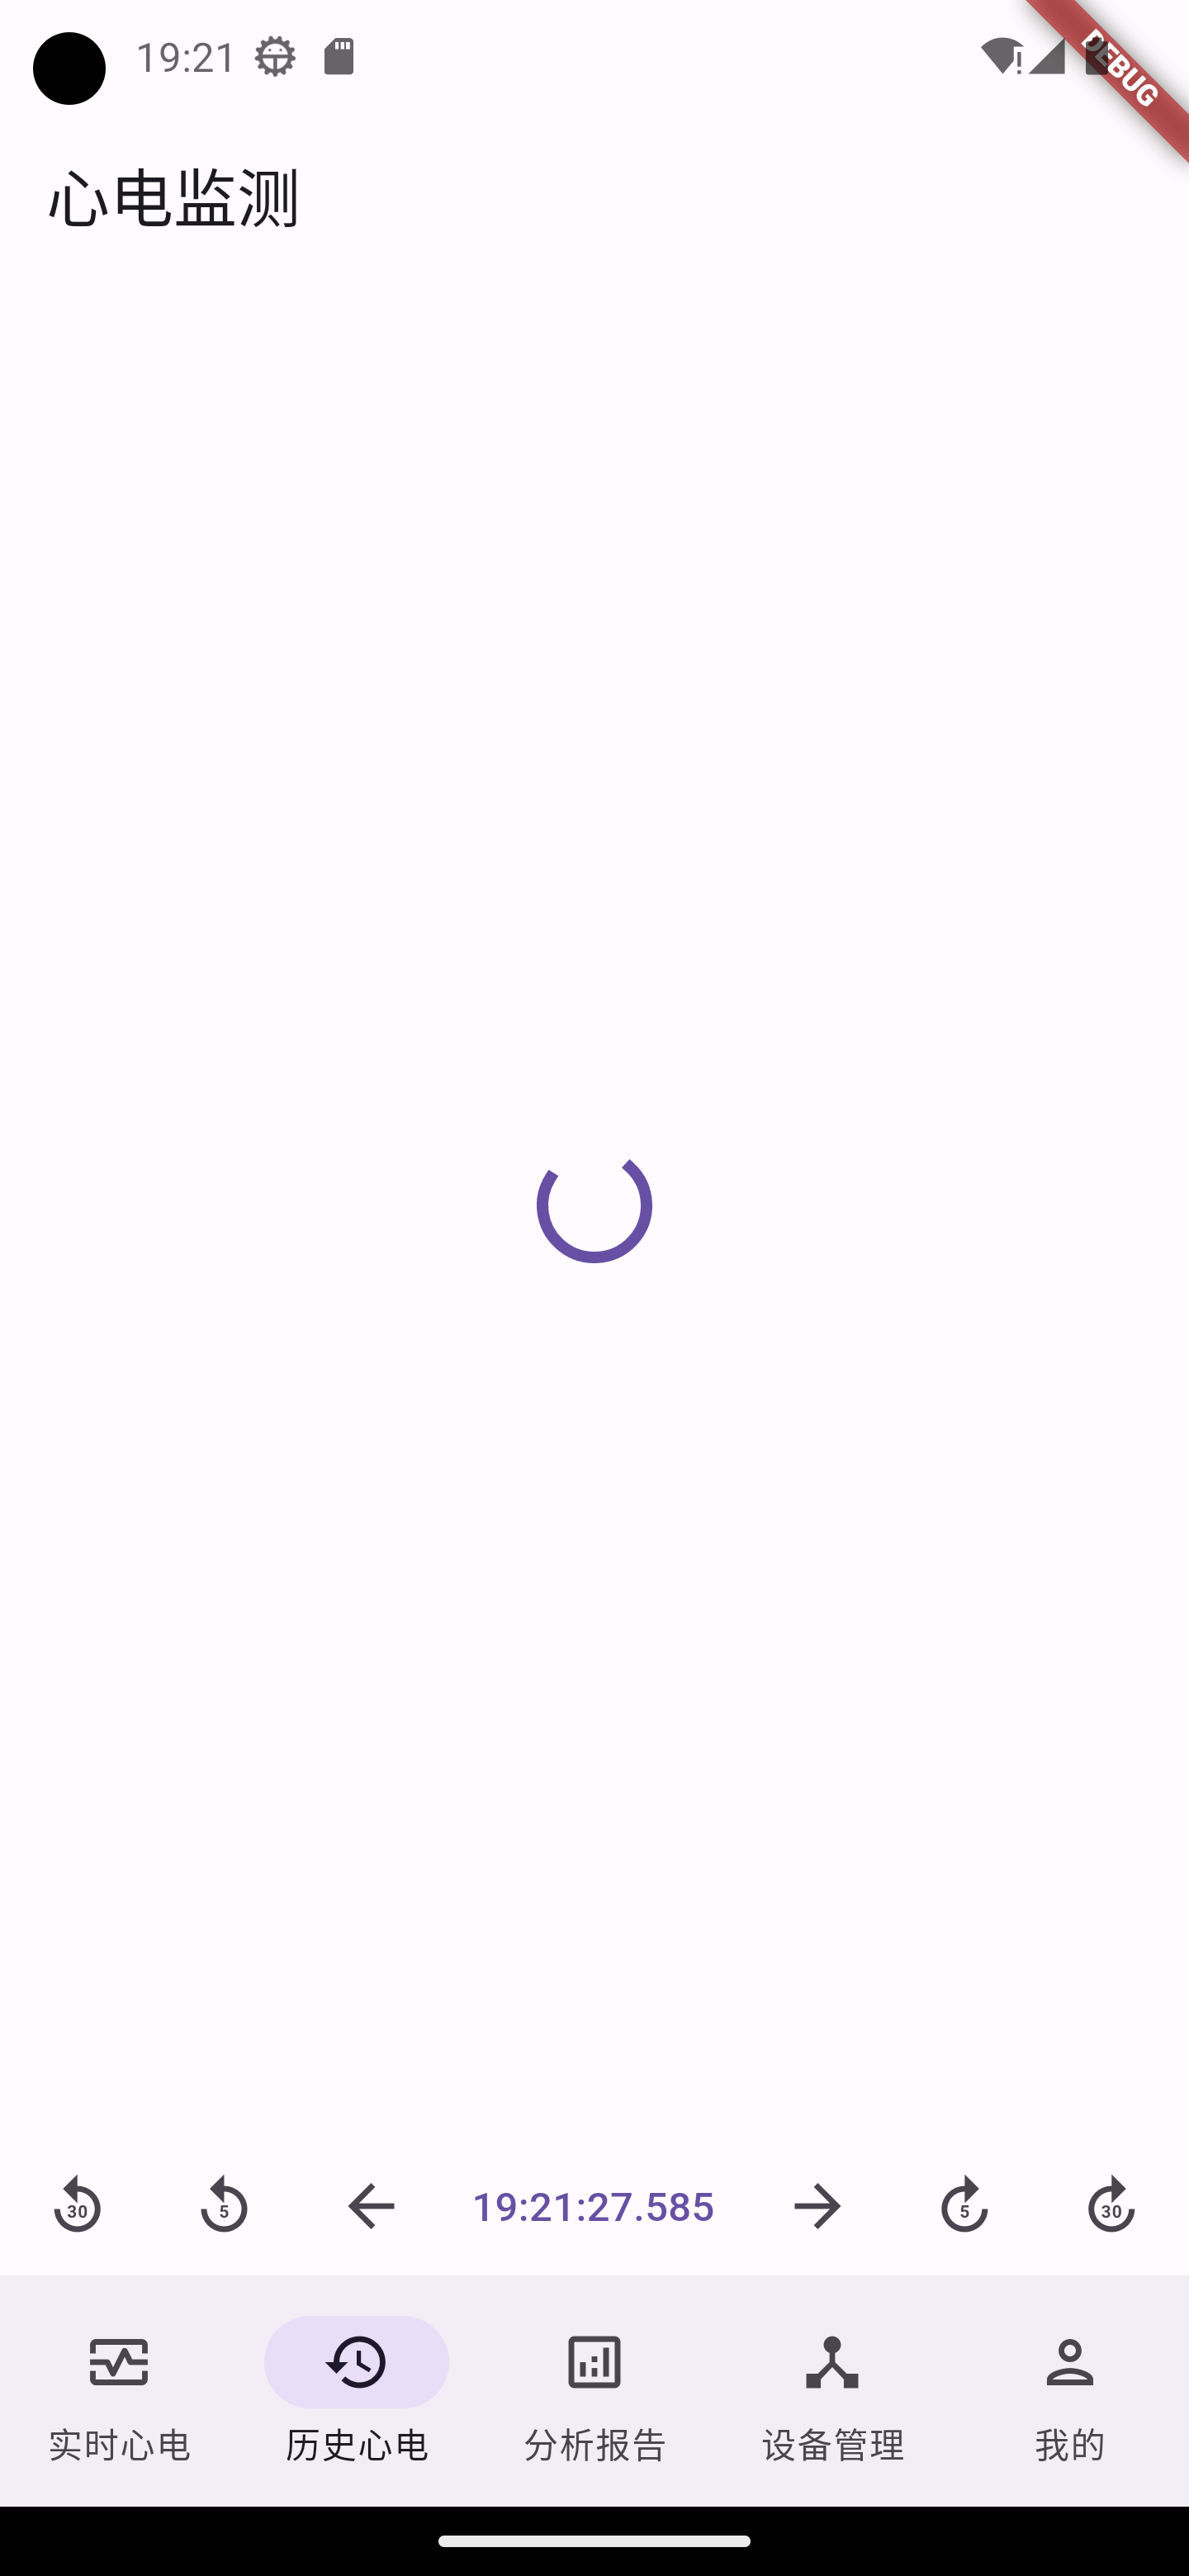
\includegraphics[width=.33\textwidth]{../assets/history-loading}}
    \subcaptionbox{正常状态}{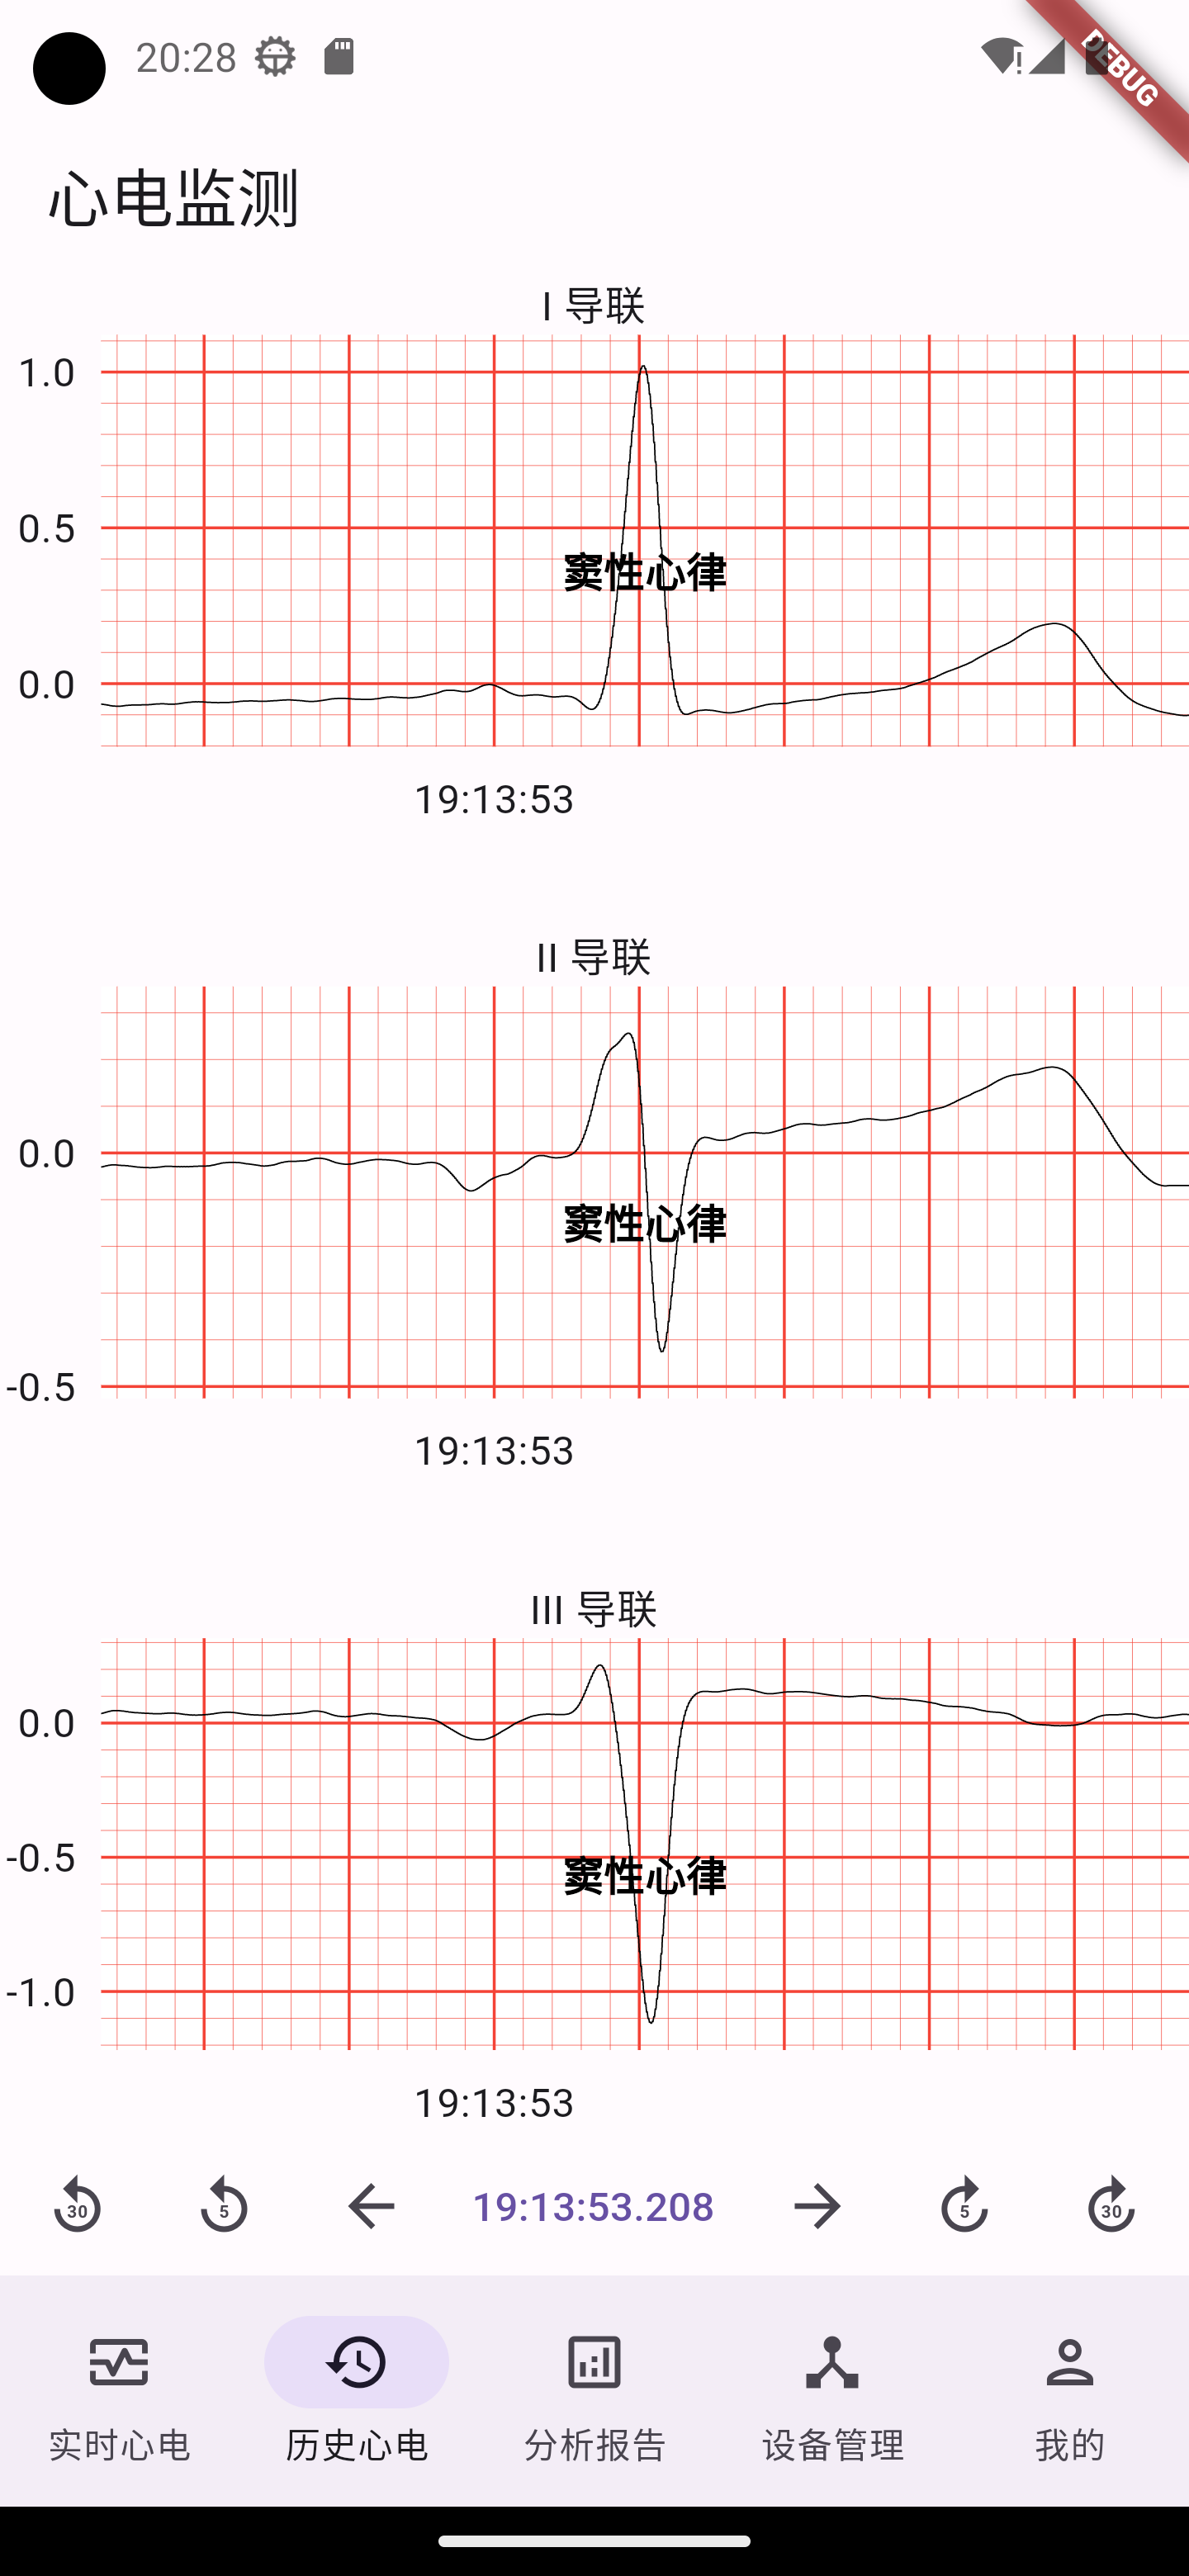
\includegraphics[width=.33\textwidth]{../assets/history}}
    \subcaptionbox{无数据}{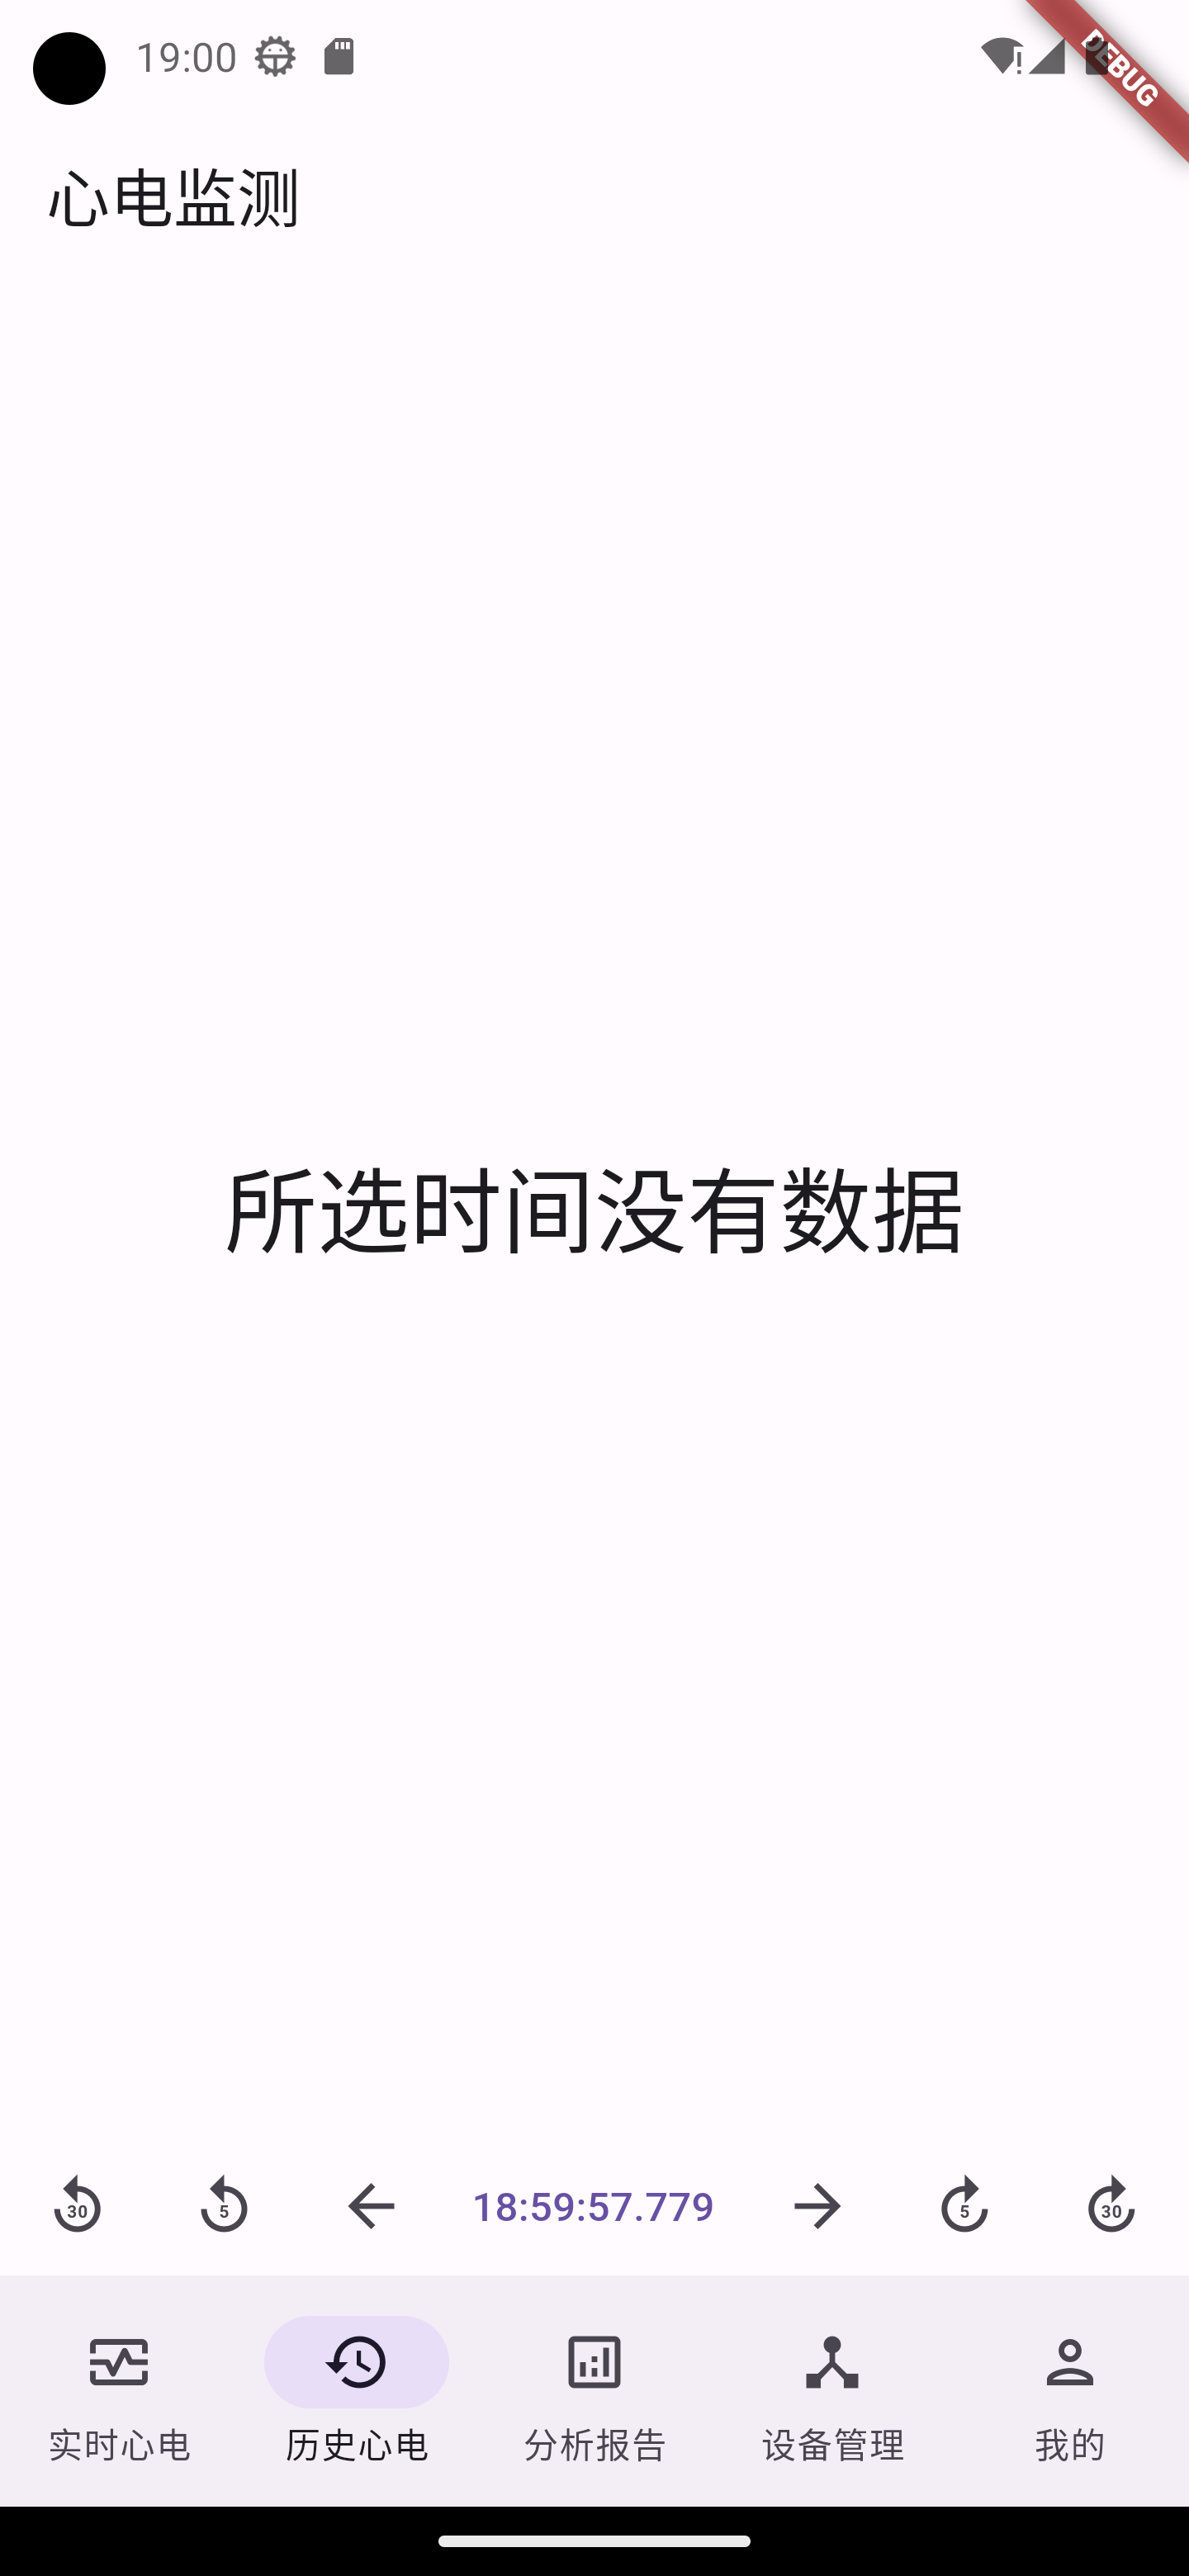
\includegraphics[width=.33\textwidth]{../assets/history-na}}
    \bicaption{历史心电界面的设计}{Design of the history ECG page}
    \label{fig:history}
\end{figure}

该界面由两部分组成,分别是上方的心电图部分和下方的时间选择器部分。

\subsubsection{心电图部分的设计}\label{subsubsec:history-ecg-design}

历史心电图与实时心电图的总体设计相同,重复部分不须赘述。相比实时心电图,历史心电图因其性质而在设计上具有一些不同点。

首先,关于心电图背景的网格,在实时心电图中完全隐去了纵线、部分显示了横线,如上文所述是因为心电图在不停横向移动。但是在历史心电图中,图中显示的数据是静态的,在用户不调整所选时间的情况下不会发生变动。因此,没有必要在历史心电图中隐去或部分隐去背景的坐标网格。在历史心电图的设计中,背景的网格线与实际的心电图纸保持一致,以粗线分割大格,每大格里再以细线(实际显示为颜色较浅的线)分割为5小格。这样的设计可以使得心电图上各点的数值更加清晰,方便用户对历史心电数据进行仔细查看。

另一个显著的不同点在于历史心电图中对每个心拍的类型进行了标注。由于所使用的智能检测算法是离线算法,无法实时给出心拍类型,因此该标注在实时心电图中无法实现,仅可在历史心电图中进行查看。心拍的类型以文本形式直接显示在每个导联的心电图中对应位置的中央。一个被考虑过的替代方案是在R波(心电图中幅度最大的波)的波峰所在的点进行标注,但这需要心电图中在上方保留一些额外的空间,不太适合移动设备的较小的屏幕,而且各个导联中的波峰也并非完全同步。另一个可能的替代方案是使用颜色而非文本对心拍类型进行标注,但这种方案要么需要在屏幕上的某处显示各种颜色对应的标签而不适合小屏幕设备,要么需要用户在某个说明页面中查看并记忆各种标签的颜色而严重影响了应用的易用性,因此也没有采用。

\subsubsection{时间选择器部分的设计}\label{subsubsec:history-time-picker-design}

\todo{时间选择器}

\begin{figure}[ht]
    \centering
    \subcaptionbox{表盘模式}{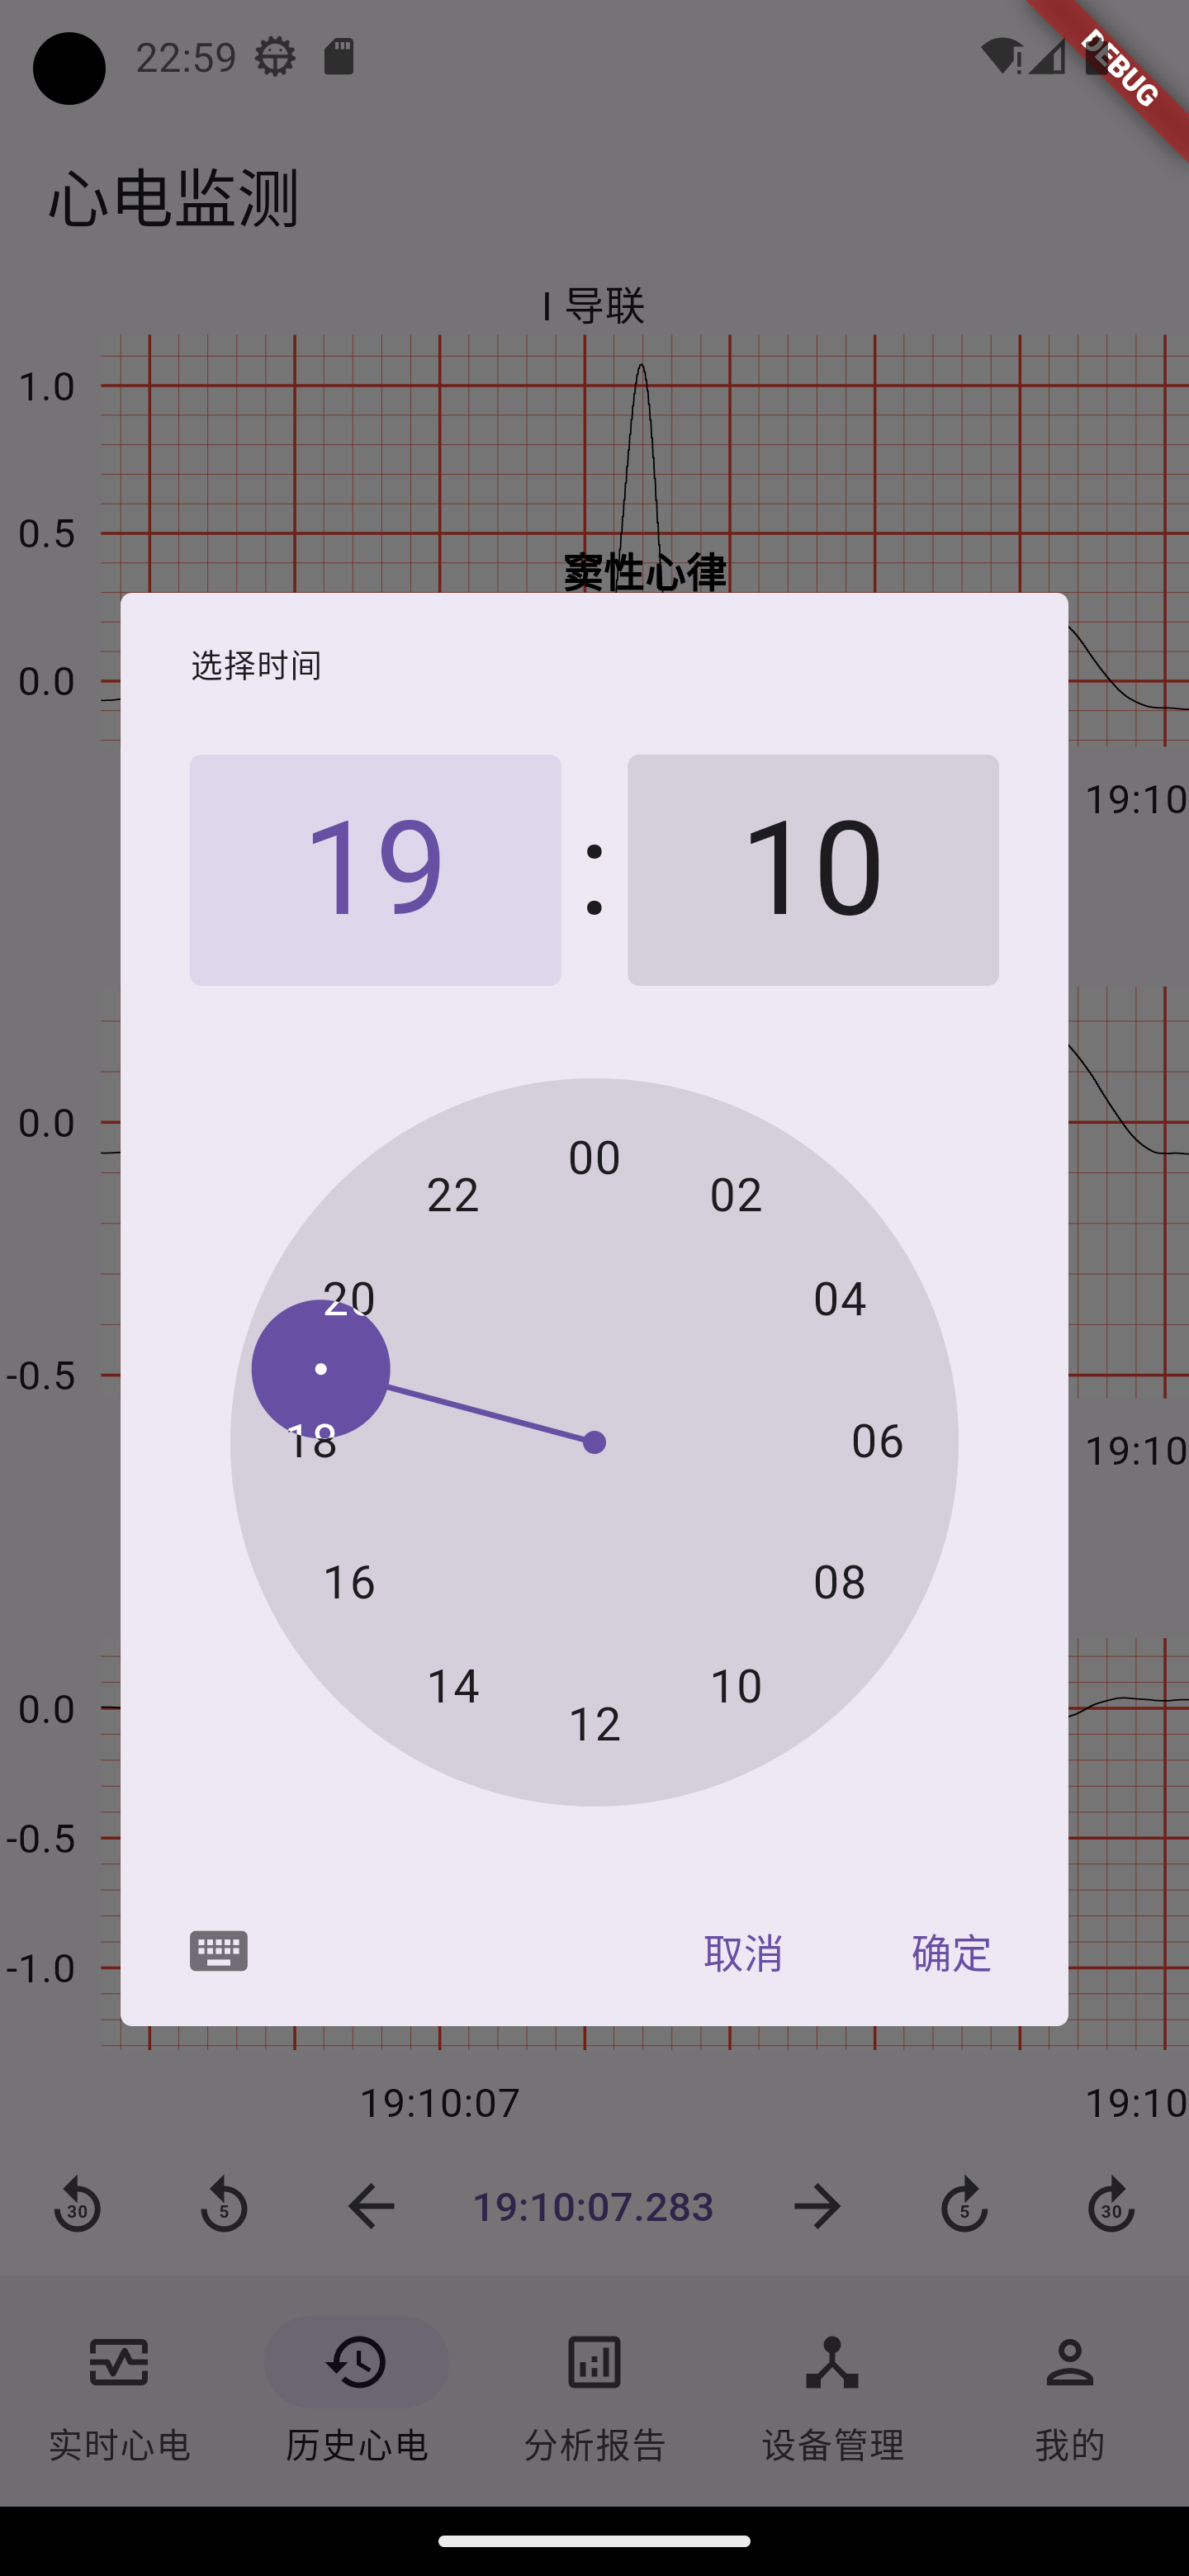
\includegraphics[width=.33\textwidth]{../assets/history-dialog-clock}}
    \subcaptionbox{数字模式}{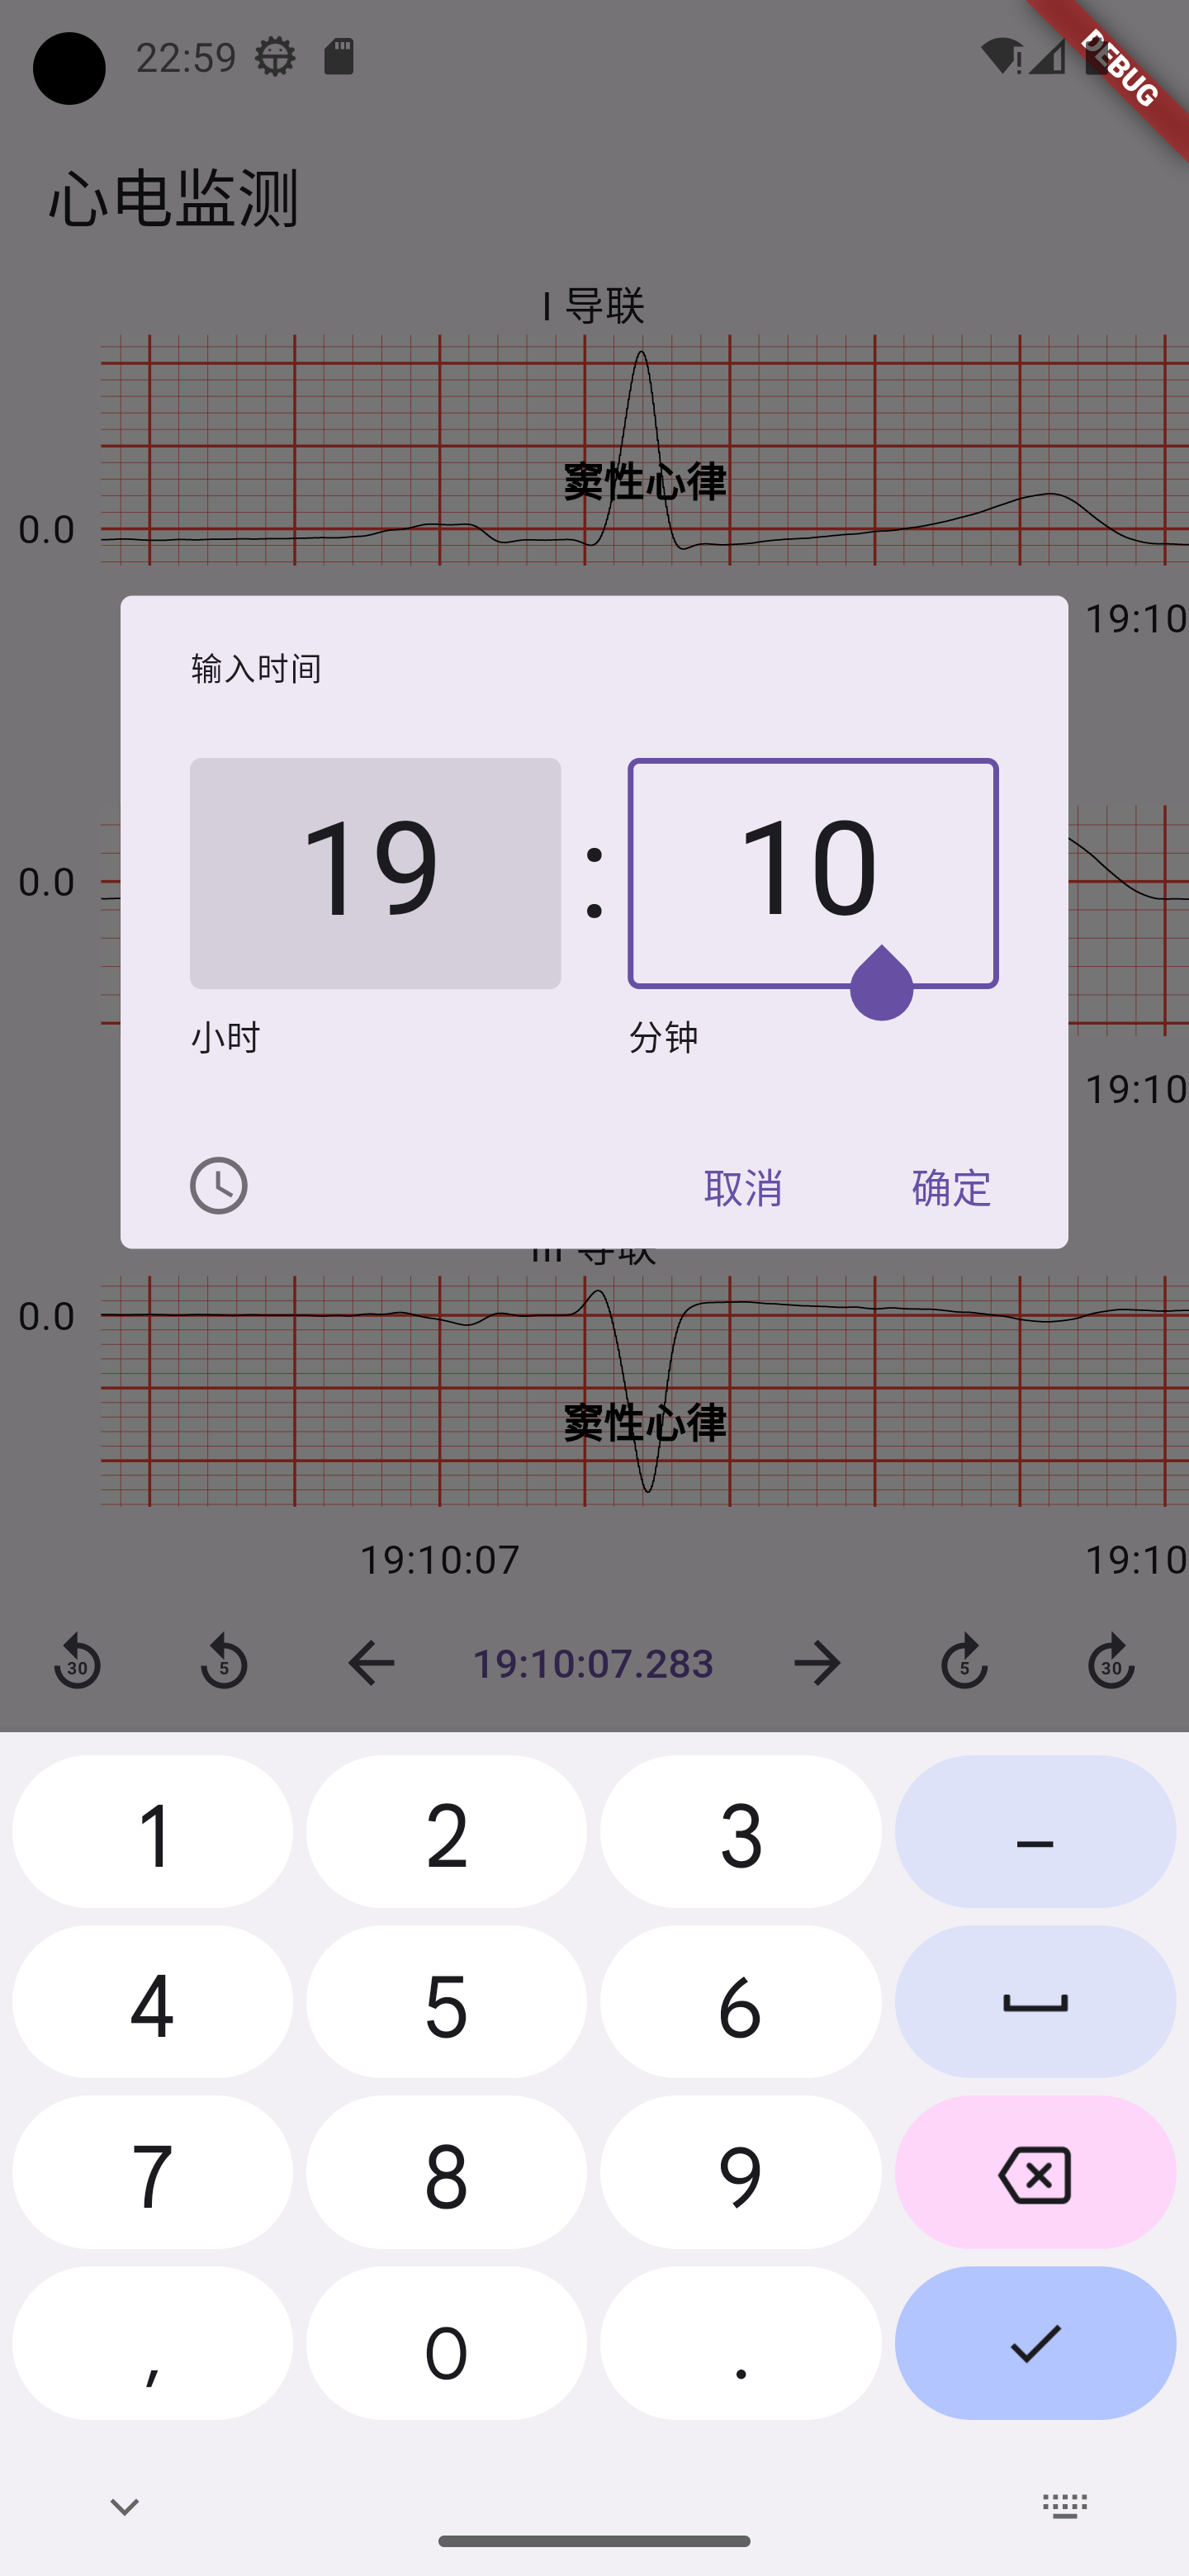
\includegraphics[width=.33\textwidth]{../assets/history-dialog-field}}
    \bicaption{历史心电时间选择器的设计}{Design of the history ECG time picker}
    \label{fig:history-time-picker}
\end{figure}

\todo{历史心电界面的设计}

\subsection{分析报告界面的设计}\label{subsec:analytics-design}

分析报告界面的整体设计如图~\ref{fig:analytics} 所示。

\begin{figure}[ht]
    \subcaptionbox{加载中}{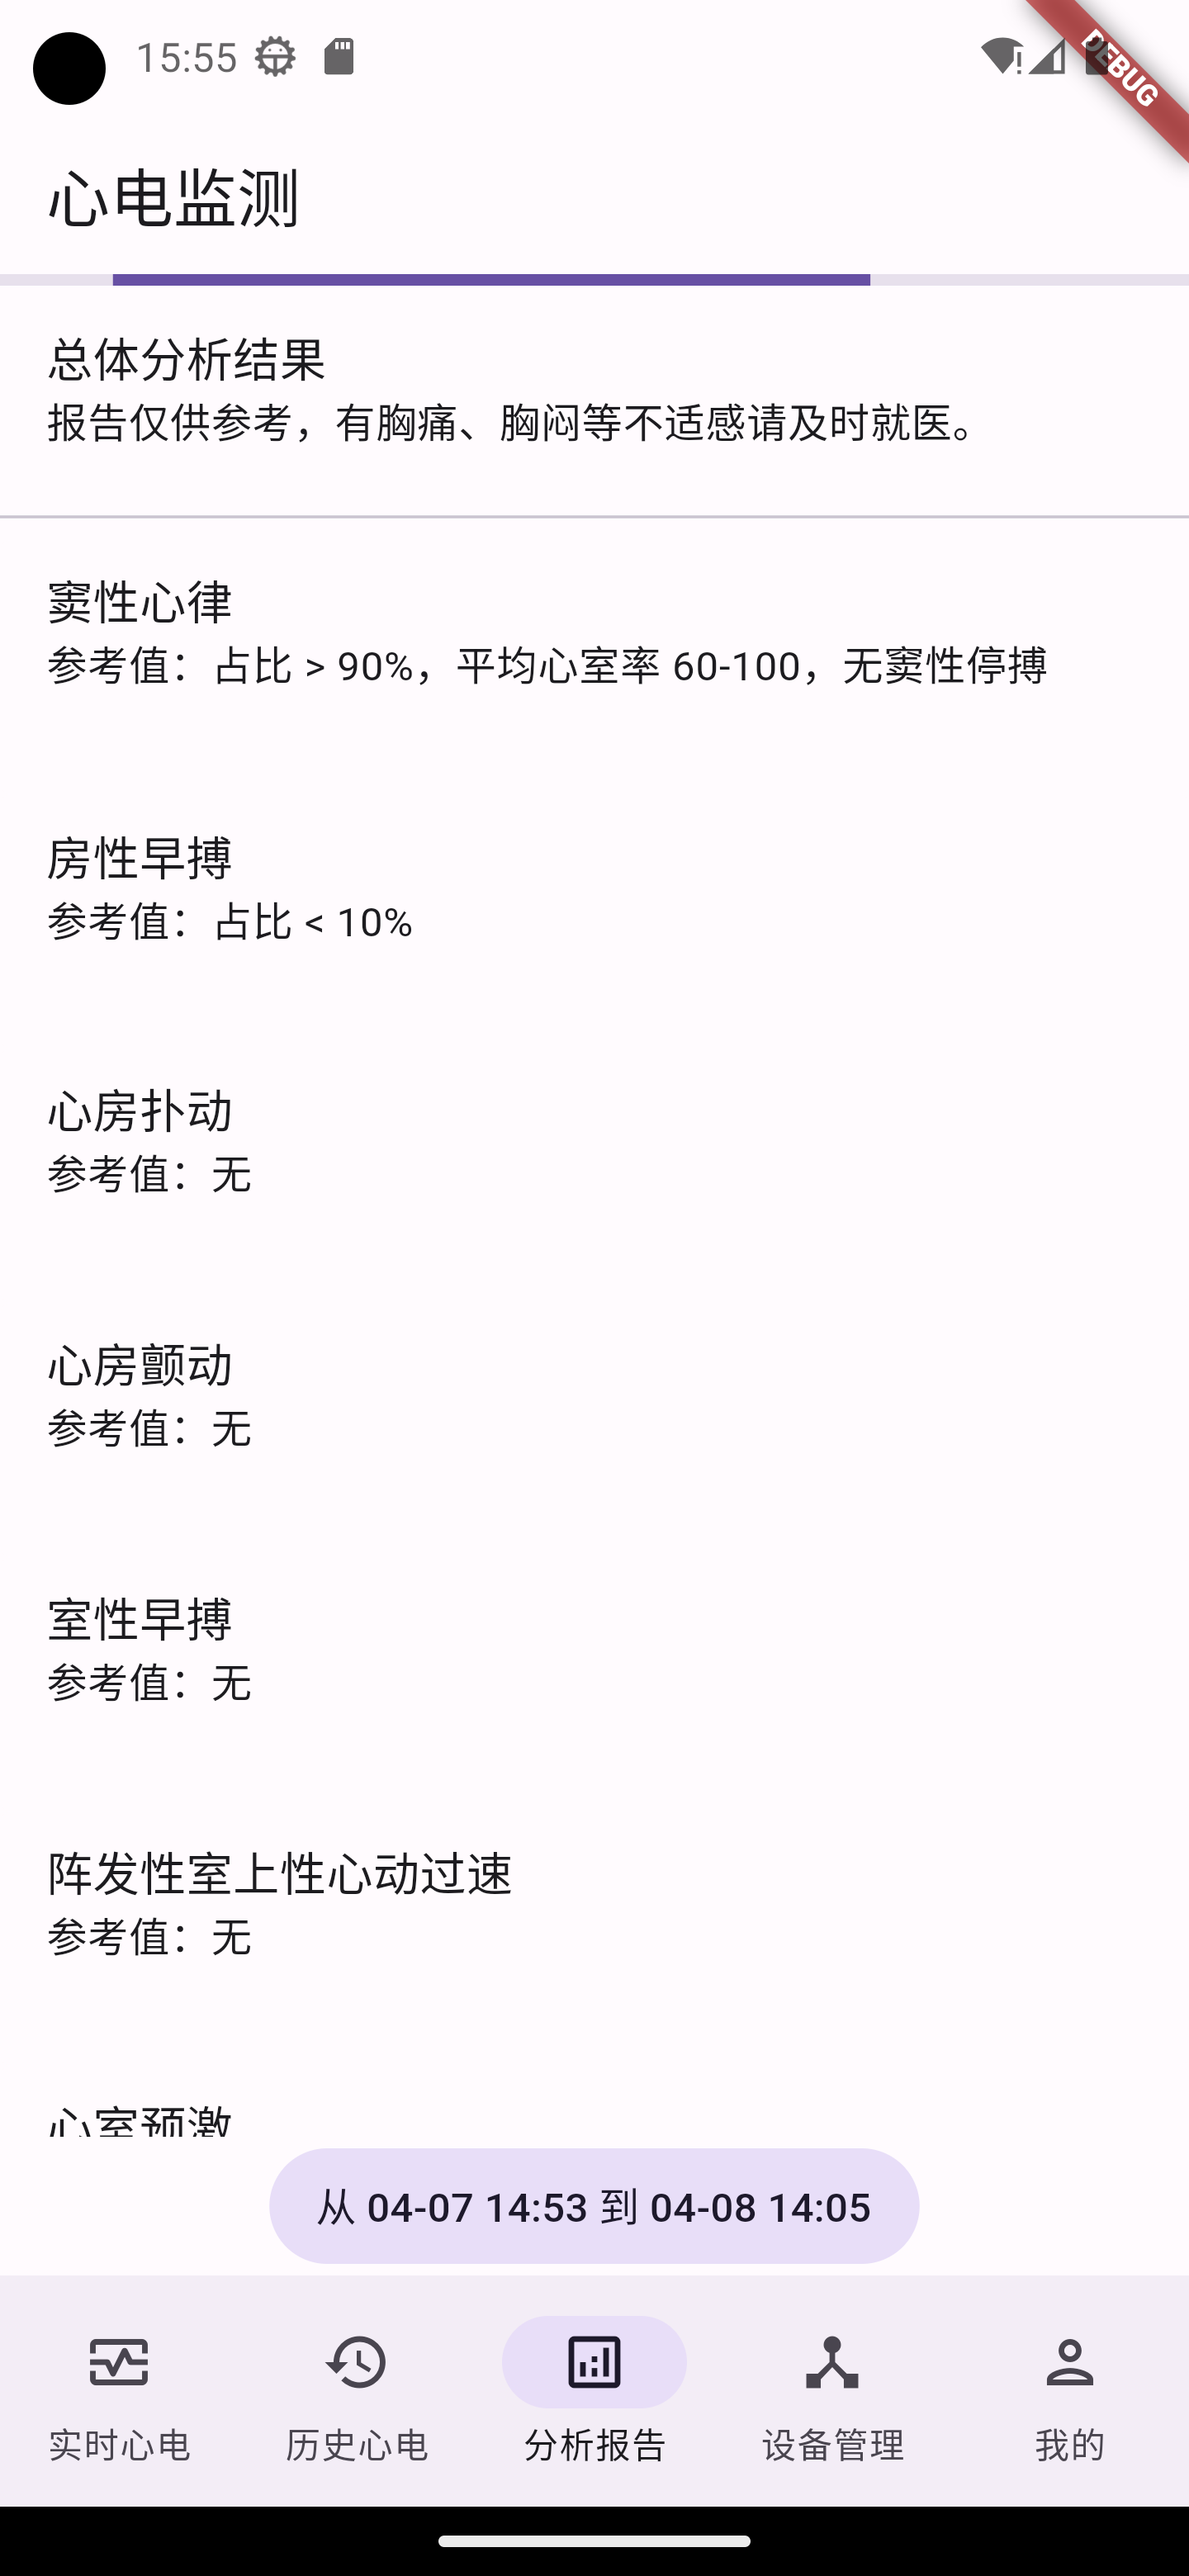
\includegraphics[width=.33\textwidth]{../assets/analytics-loading}}
    \subcaptionbox{正常状态}{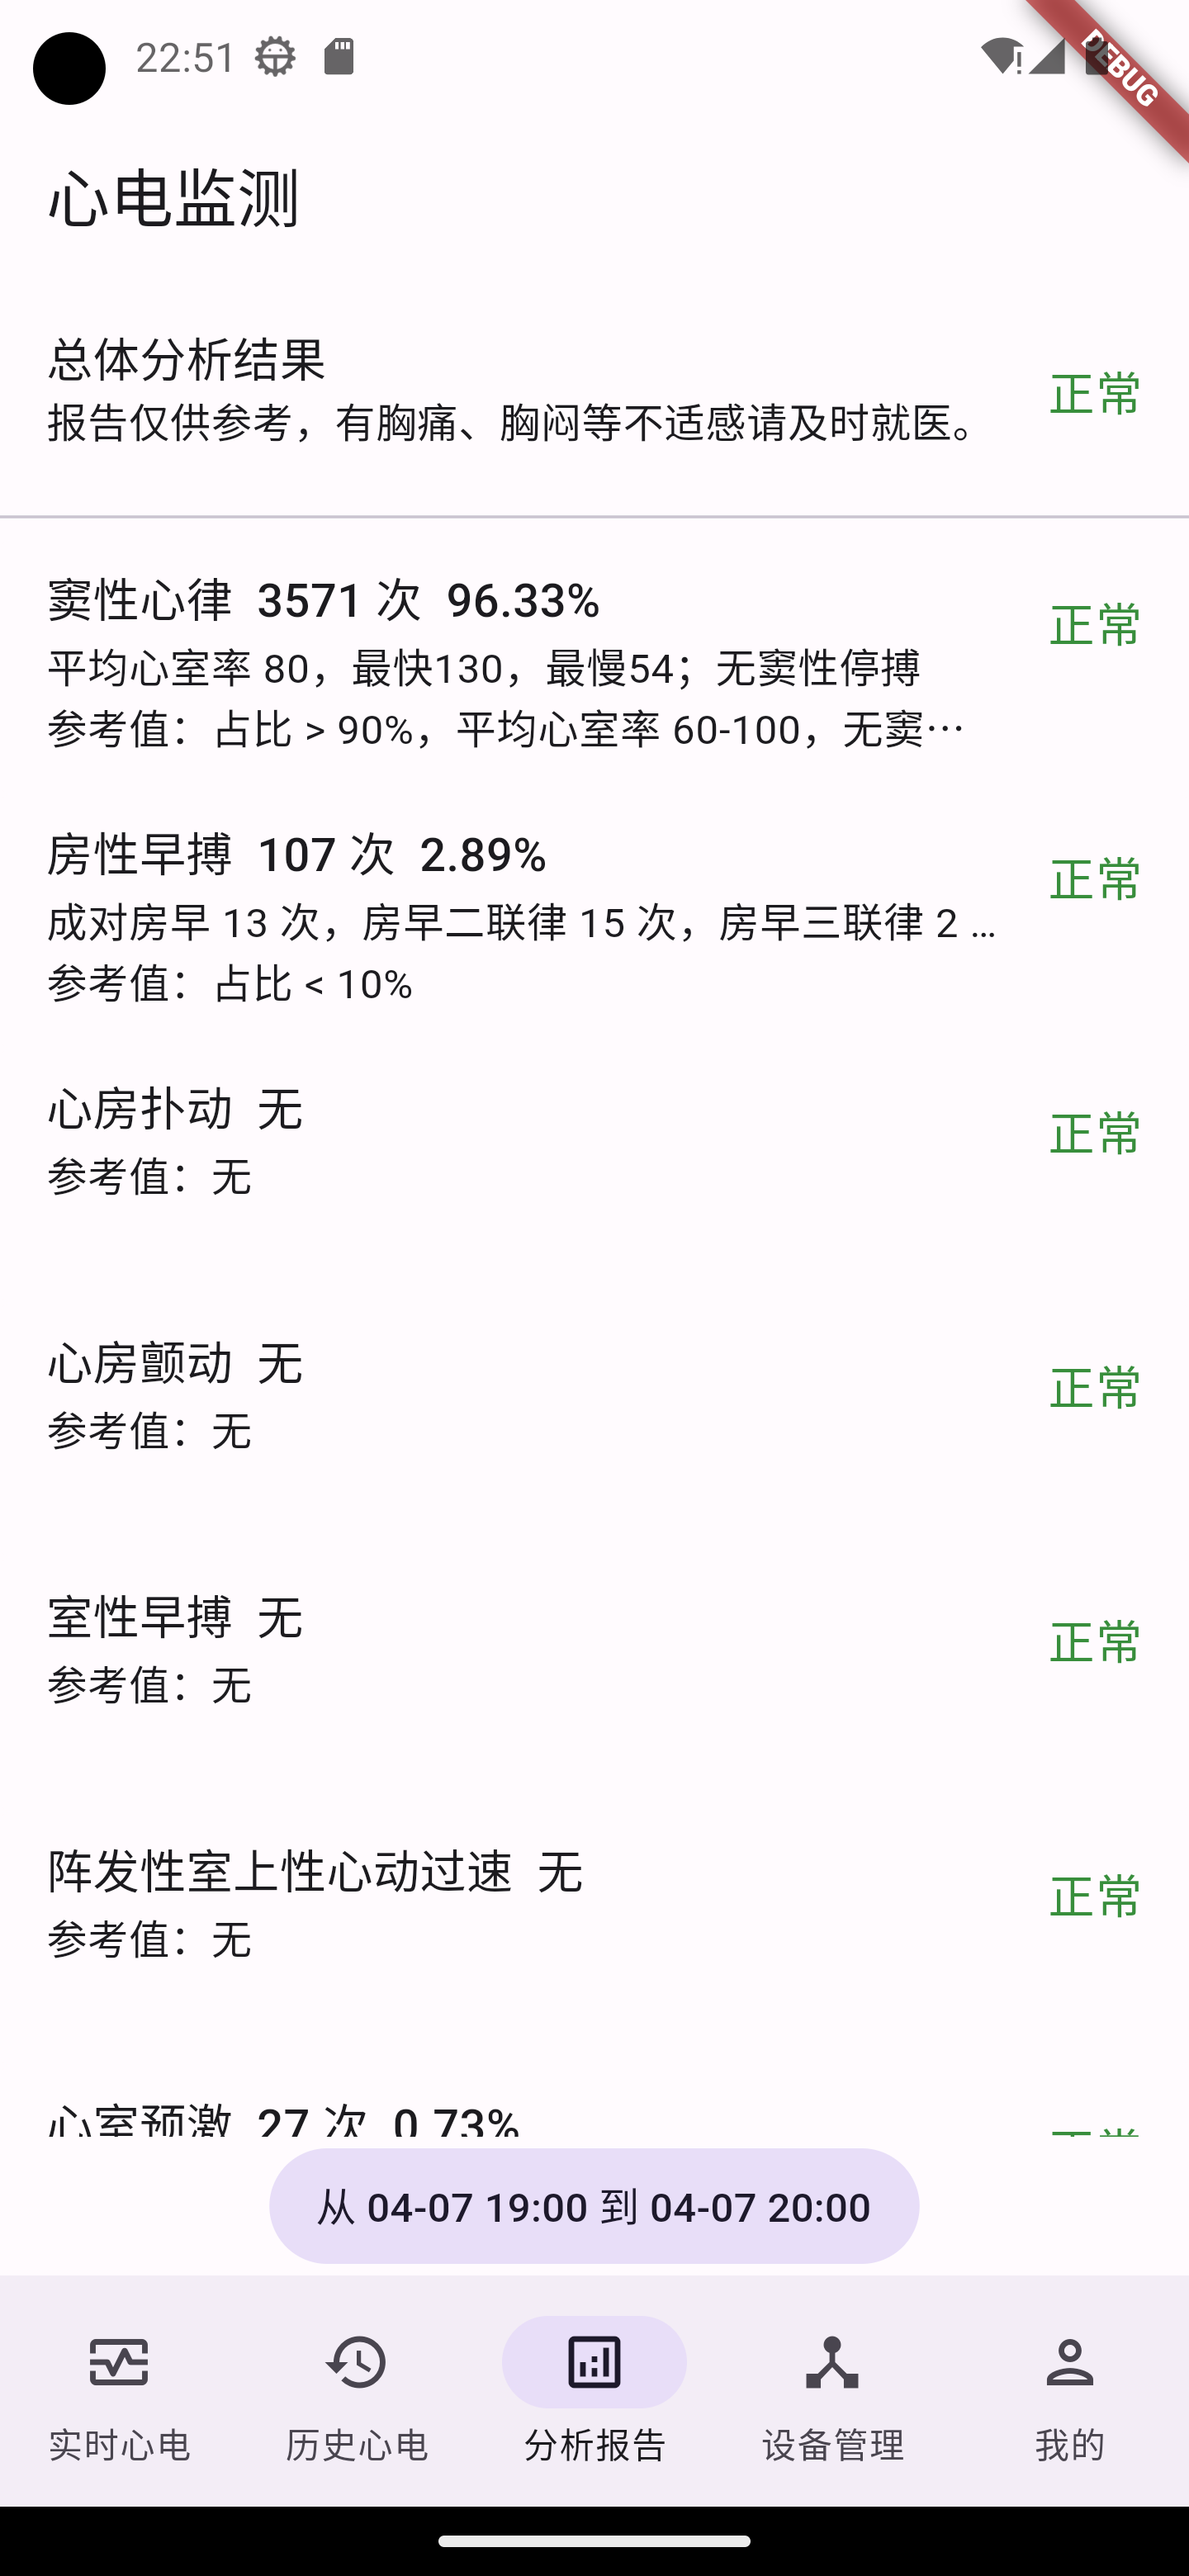
\includegraphics[width=.33\textwidth]{../assets/analytics}}
    \subcaptionbox{时间范围选择}{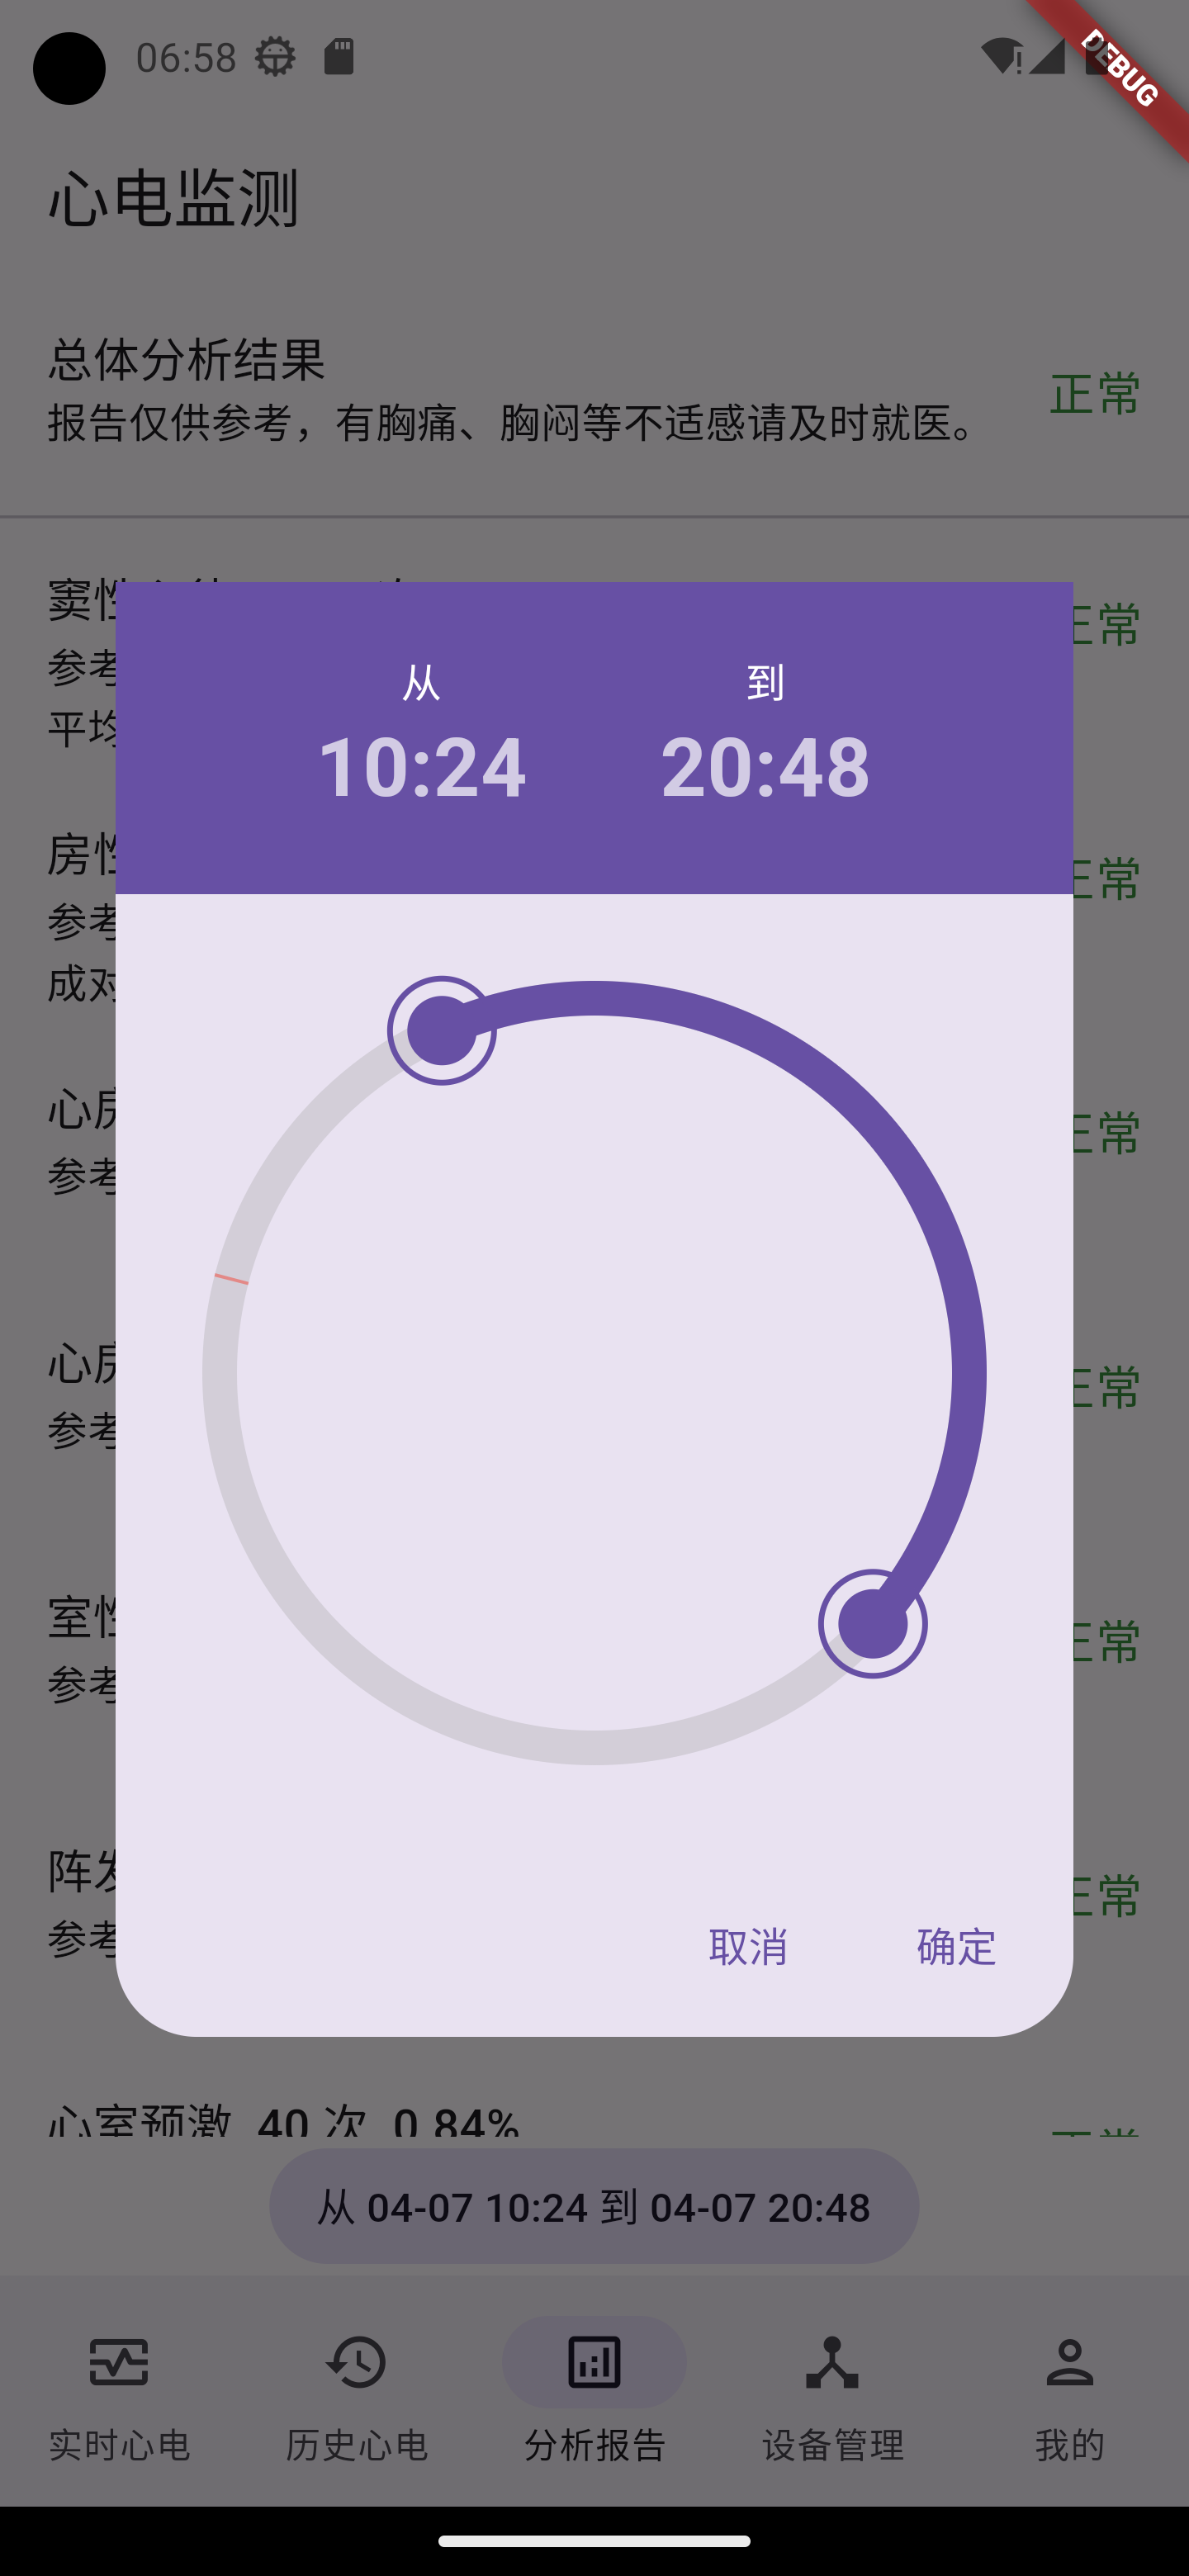
\includegraphics[width=.33\textwidth]{../assets/analytics-dialog}}
    \bicaption{分析报告界面的设计}{Design of the analytics page}
    \label{fig:analytics}
\end{figure}

\todo{分析报告界面的设计}

\subsubsection{心律类型详情界面的设计}\label{subsubsec:label-details}

\todo{心律类型详情界面的设计}

\begin{figure}[ht]
    \centering
    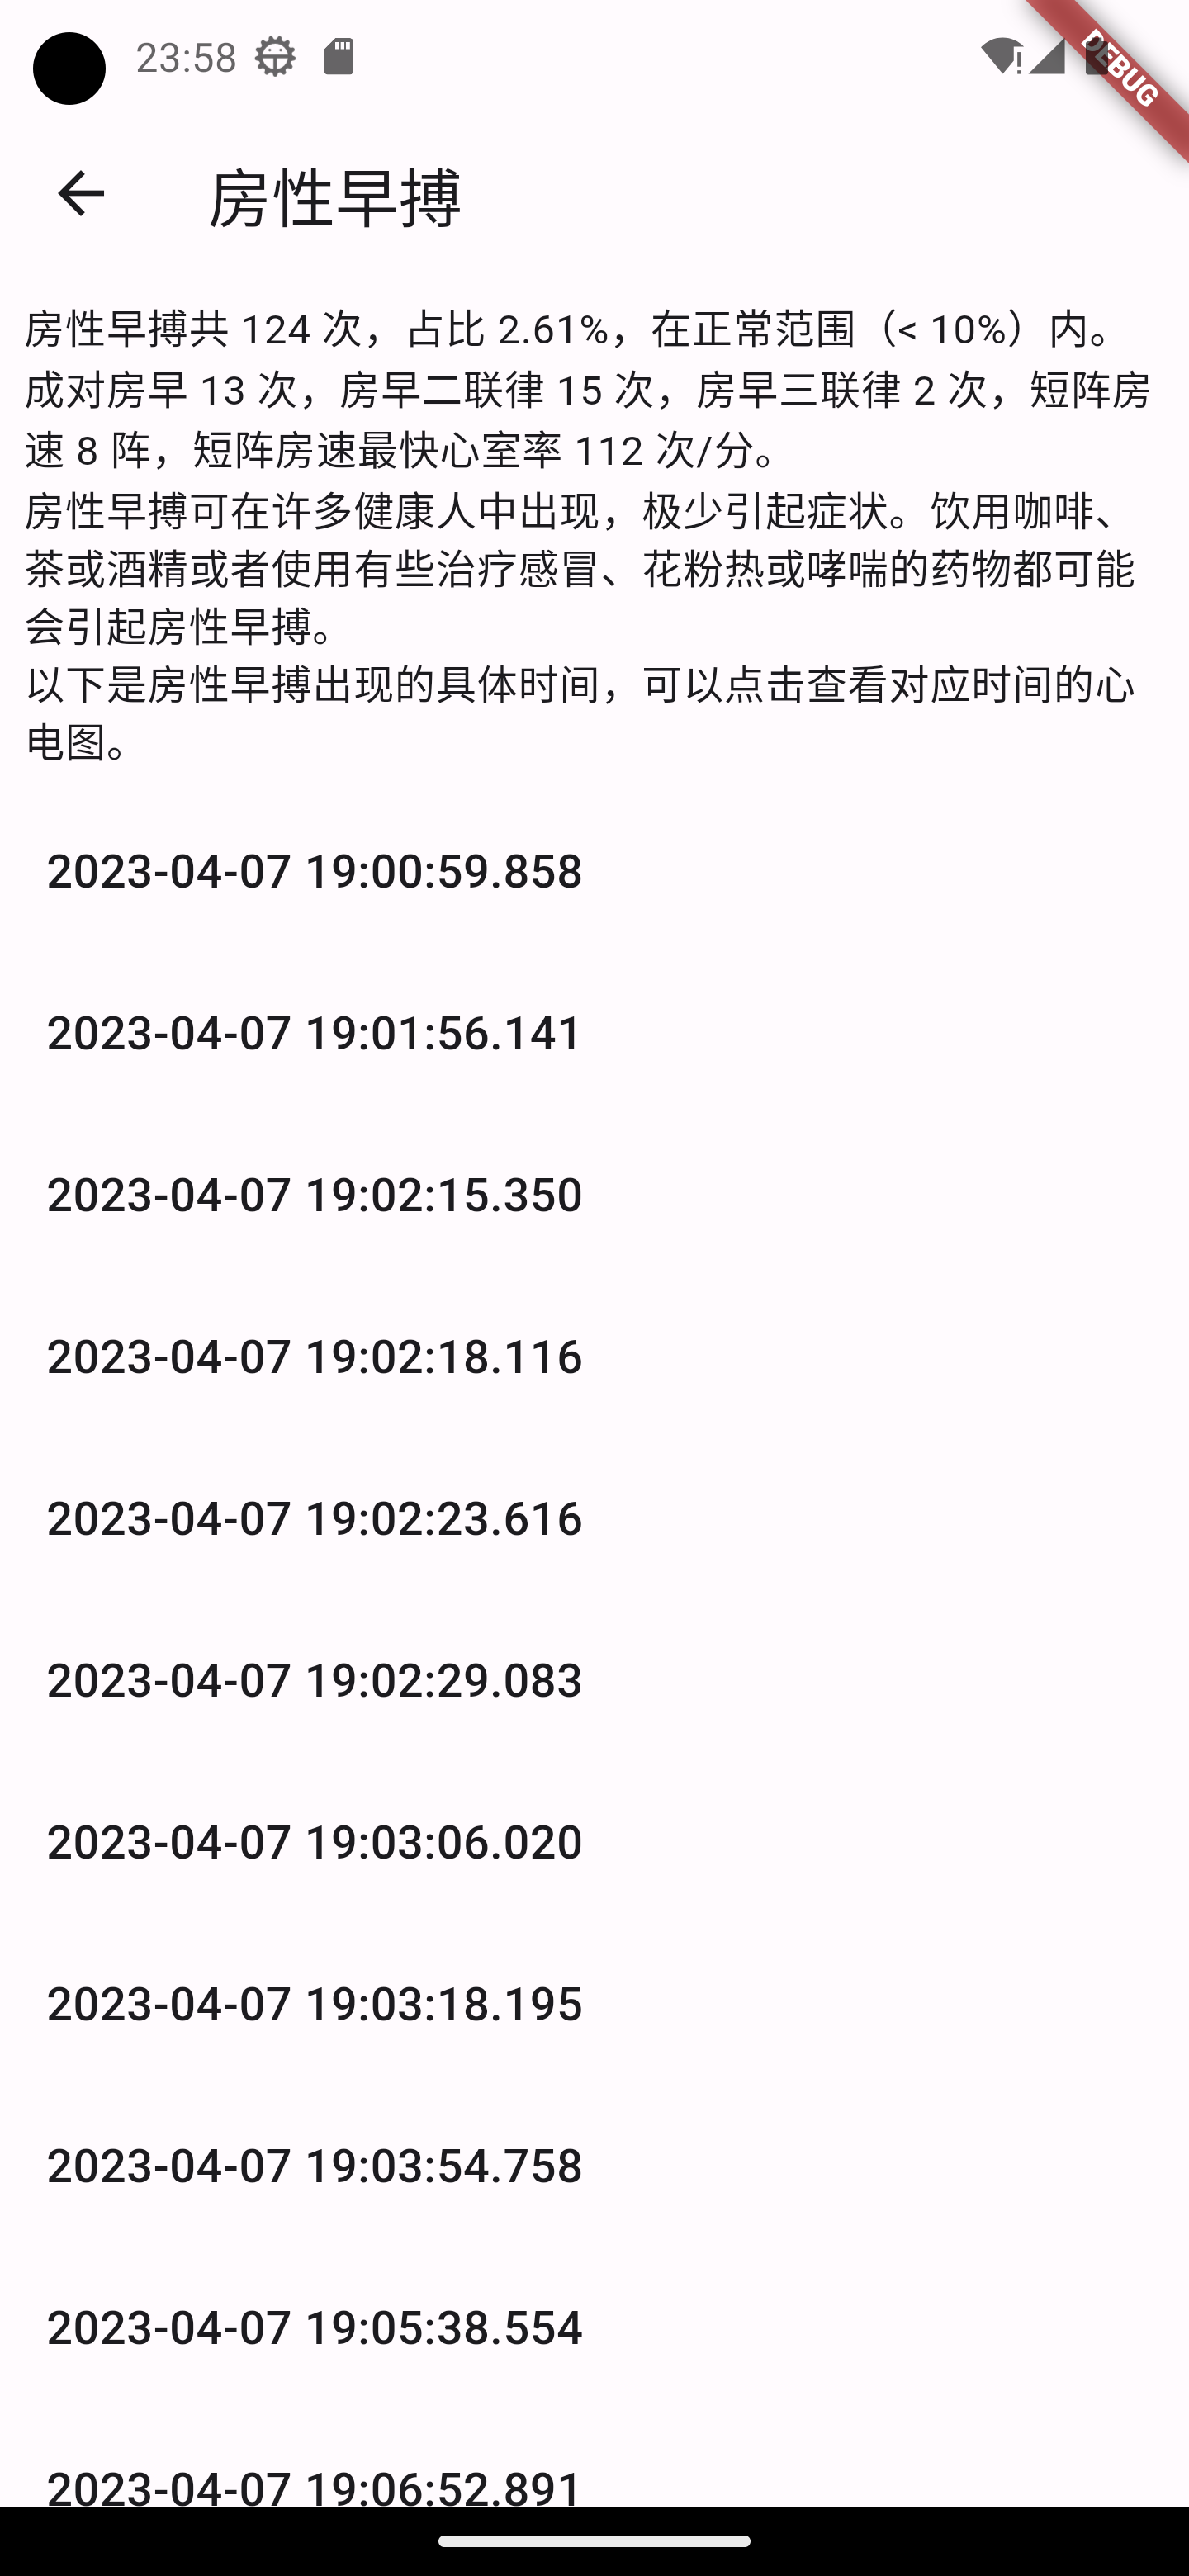
\includegraphics[width=.33\textwidth]{../assets/label-details}
    \bicaption{心律类型详情界面的设计}{Design of the heart rhythm details page}
    \label{fig:label-details}
\end{figure}

\subsection{设备管理界面的设计}\label{subsec:device-design}

设备管理界面的整体设计如图~\ref{fig:device} 所示。

\begin{figure}[ht]
    \subcaptionbox{已连接}{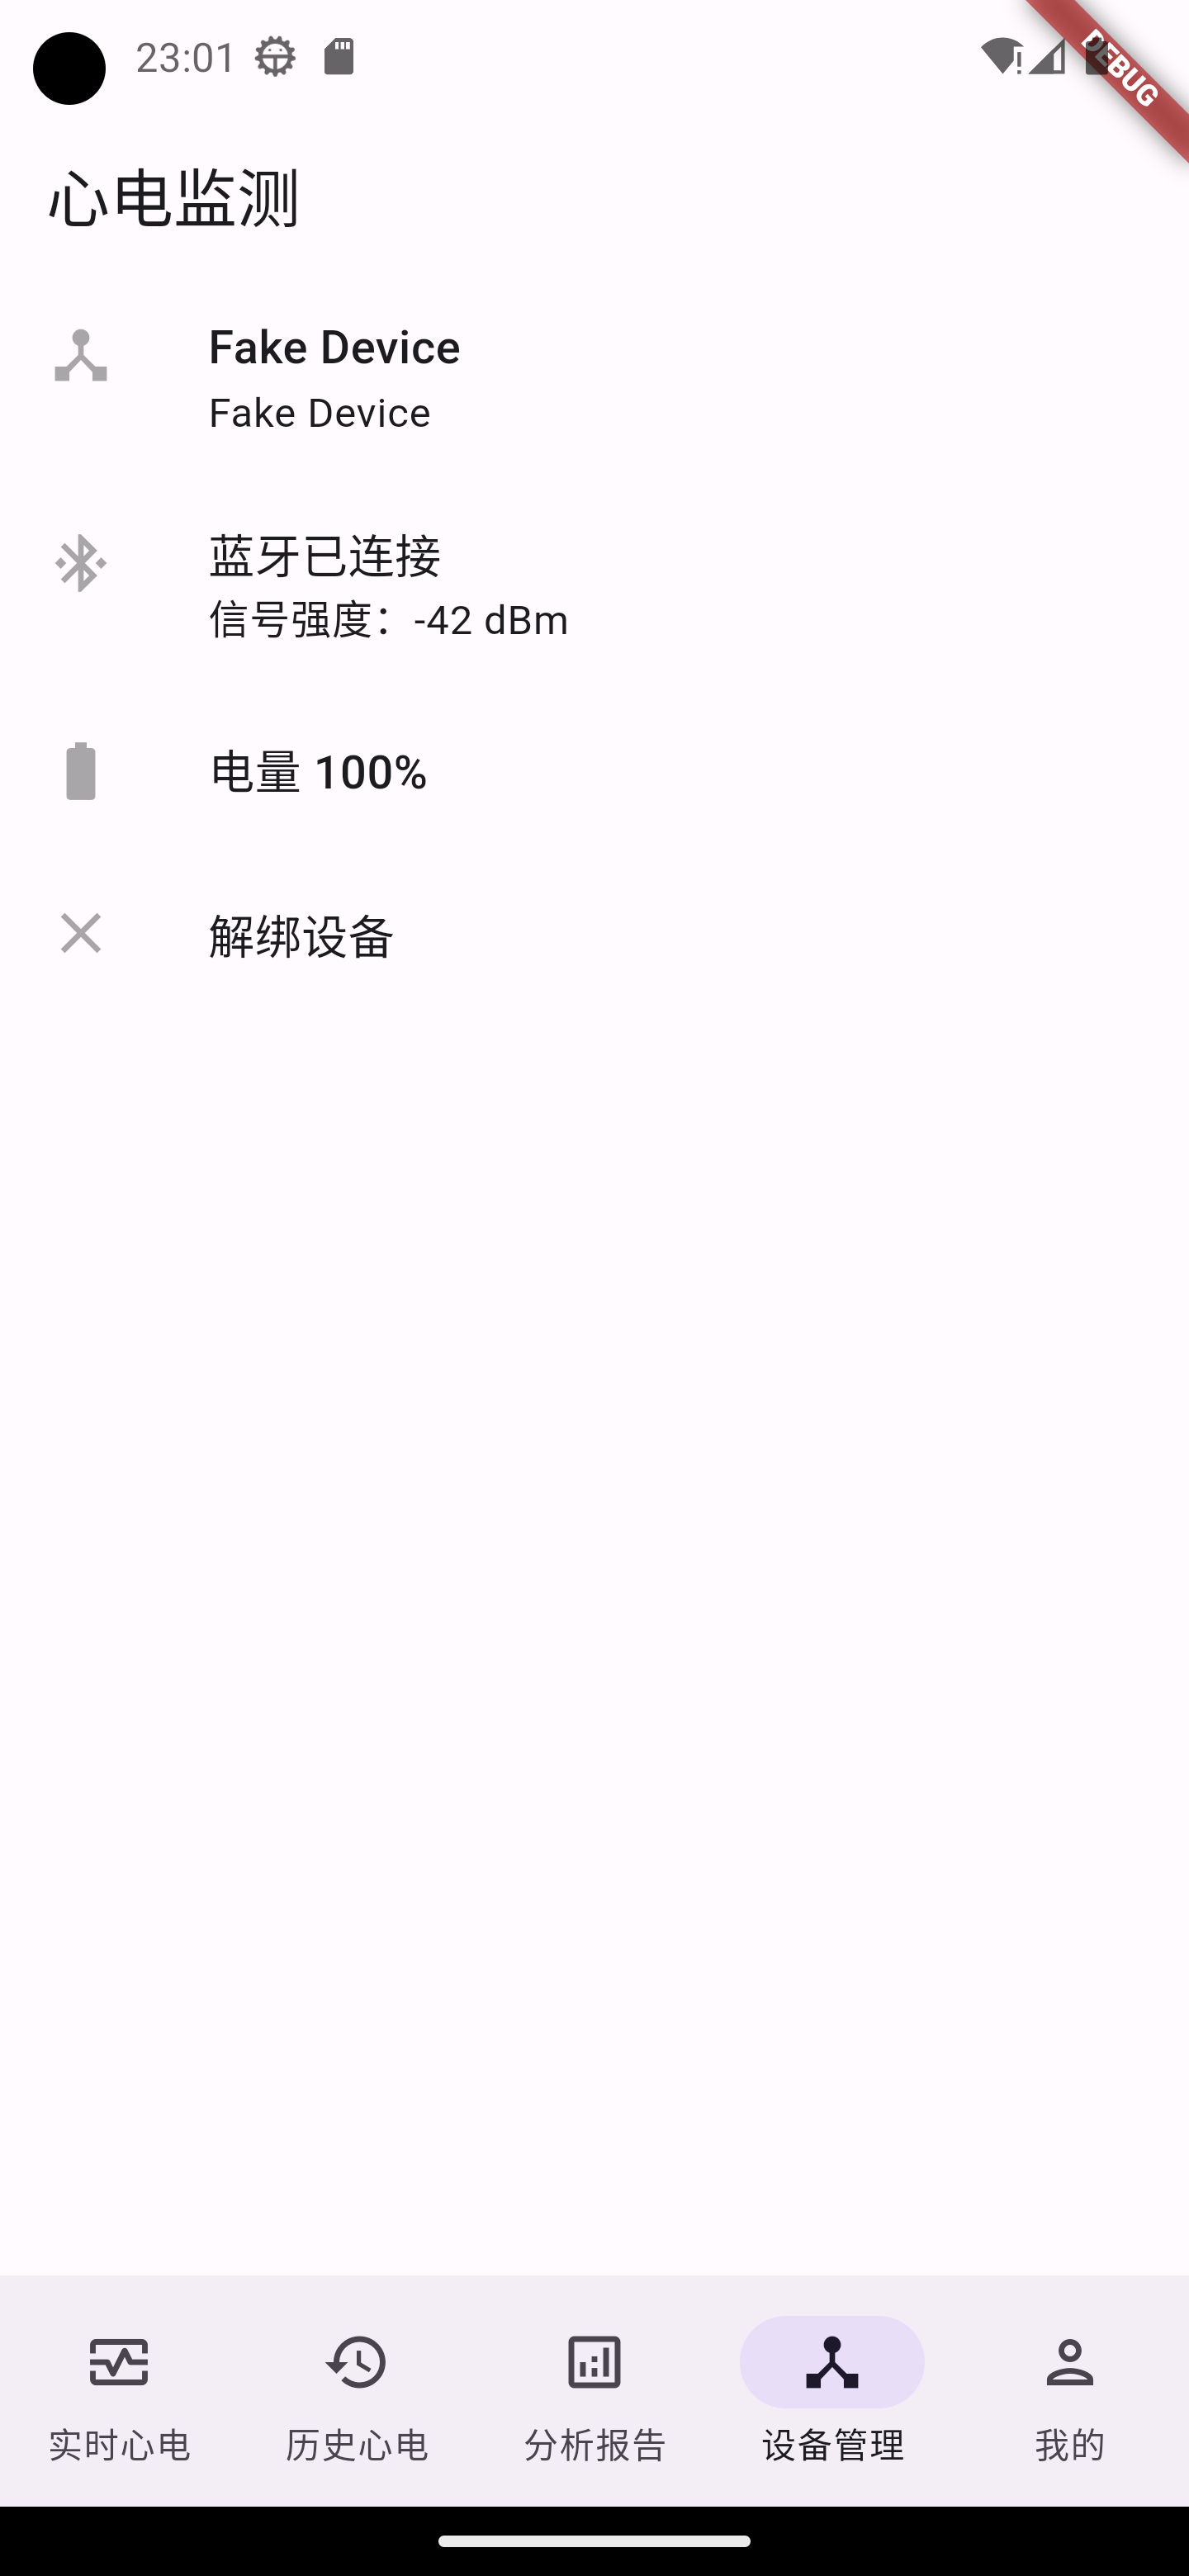
\includegraphics[width=.33\textwidth]{../assets/device-connected}}
    \subcaptionbox{连接新设备}{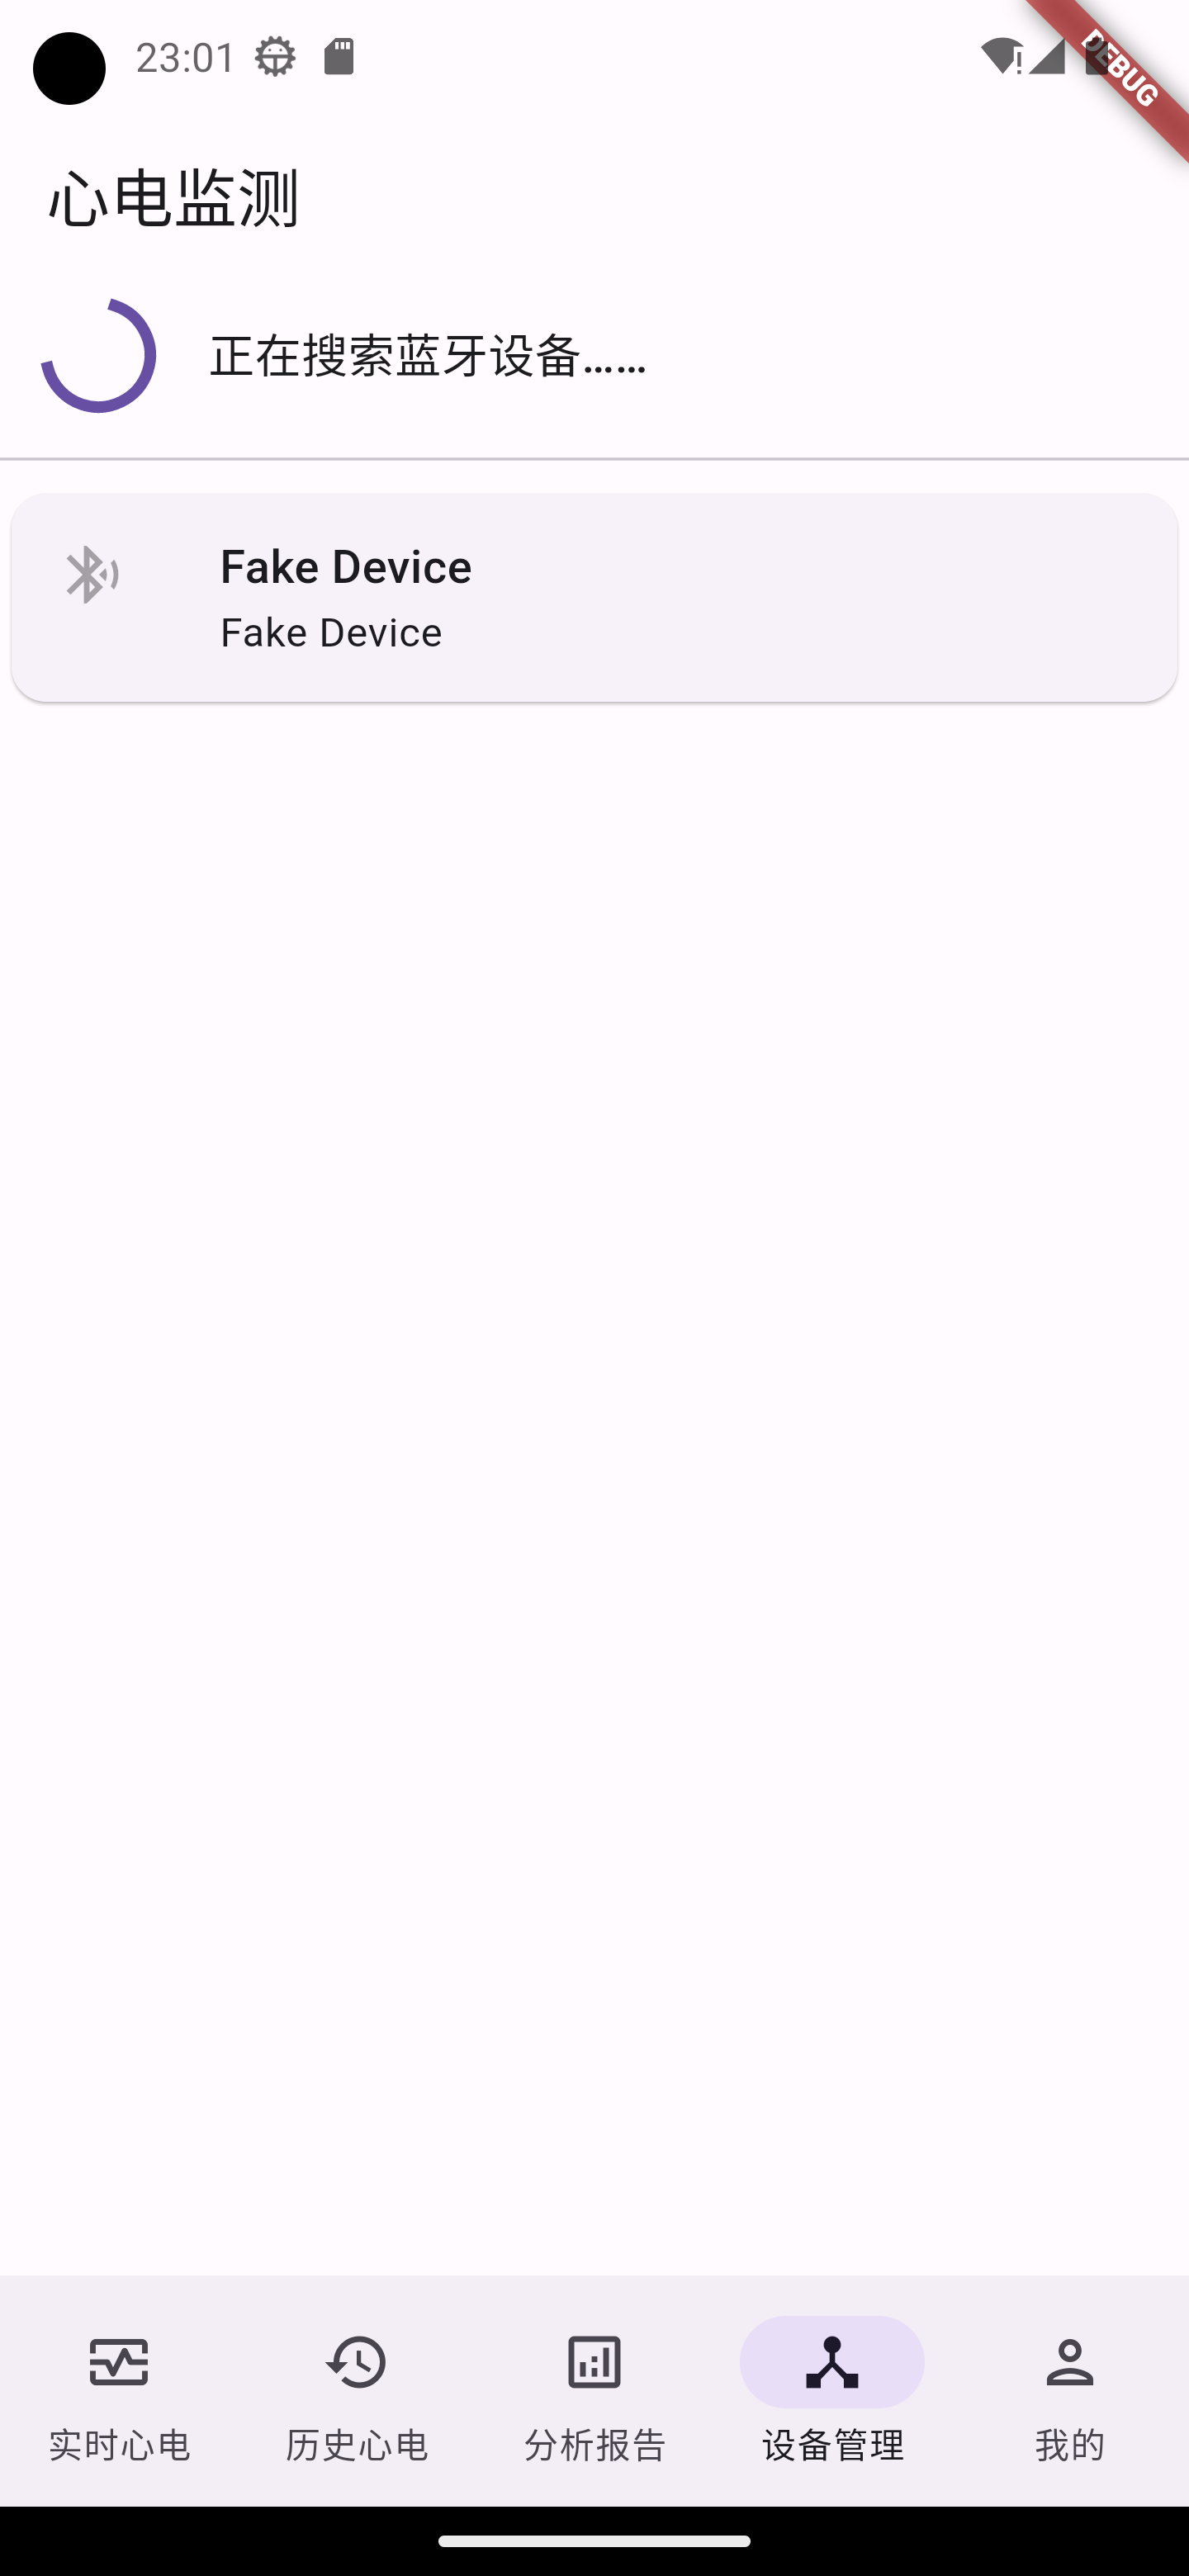
\includegraphics[width=.33\textwidth]{../assets/device-new}}
    \subcaptionbox{无可用设备}{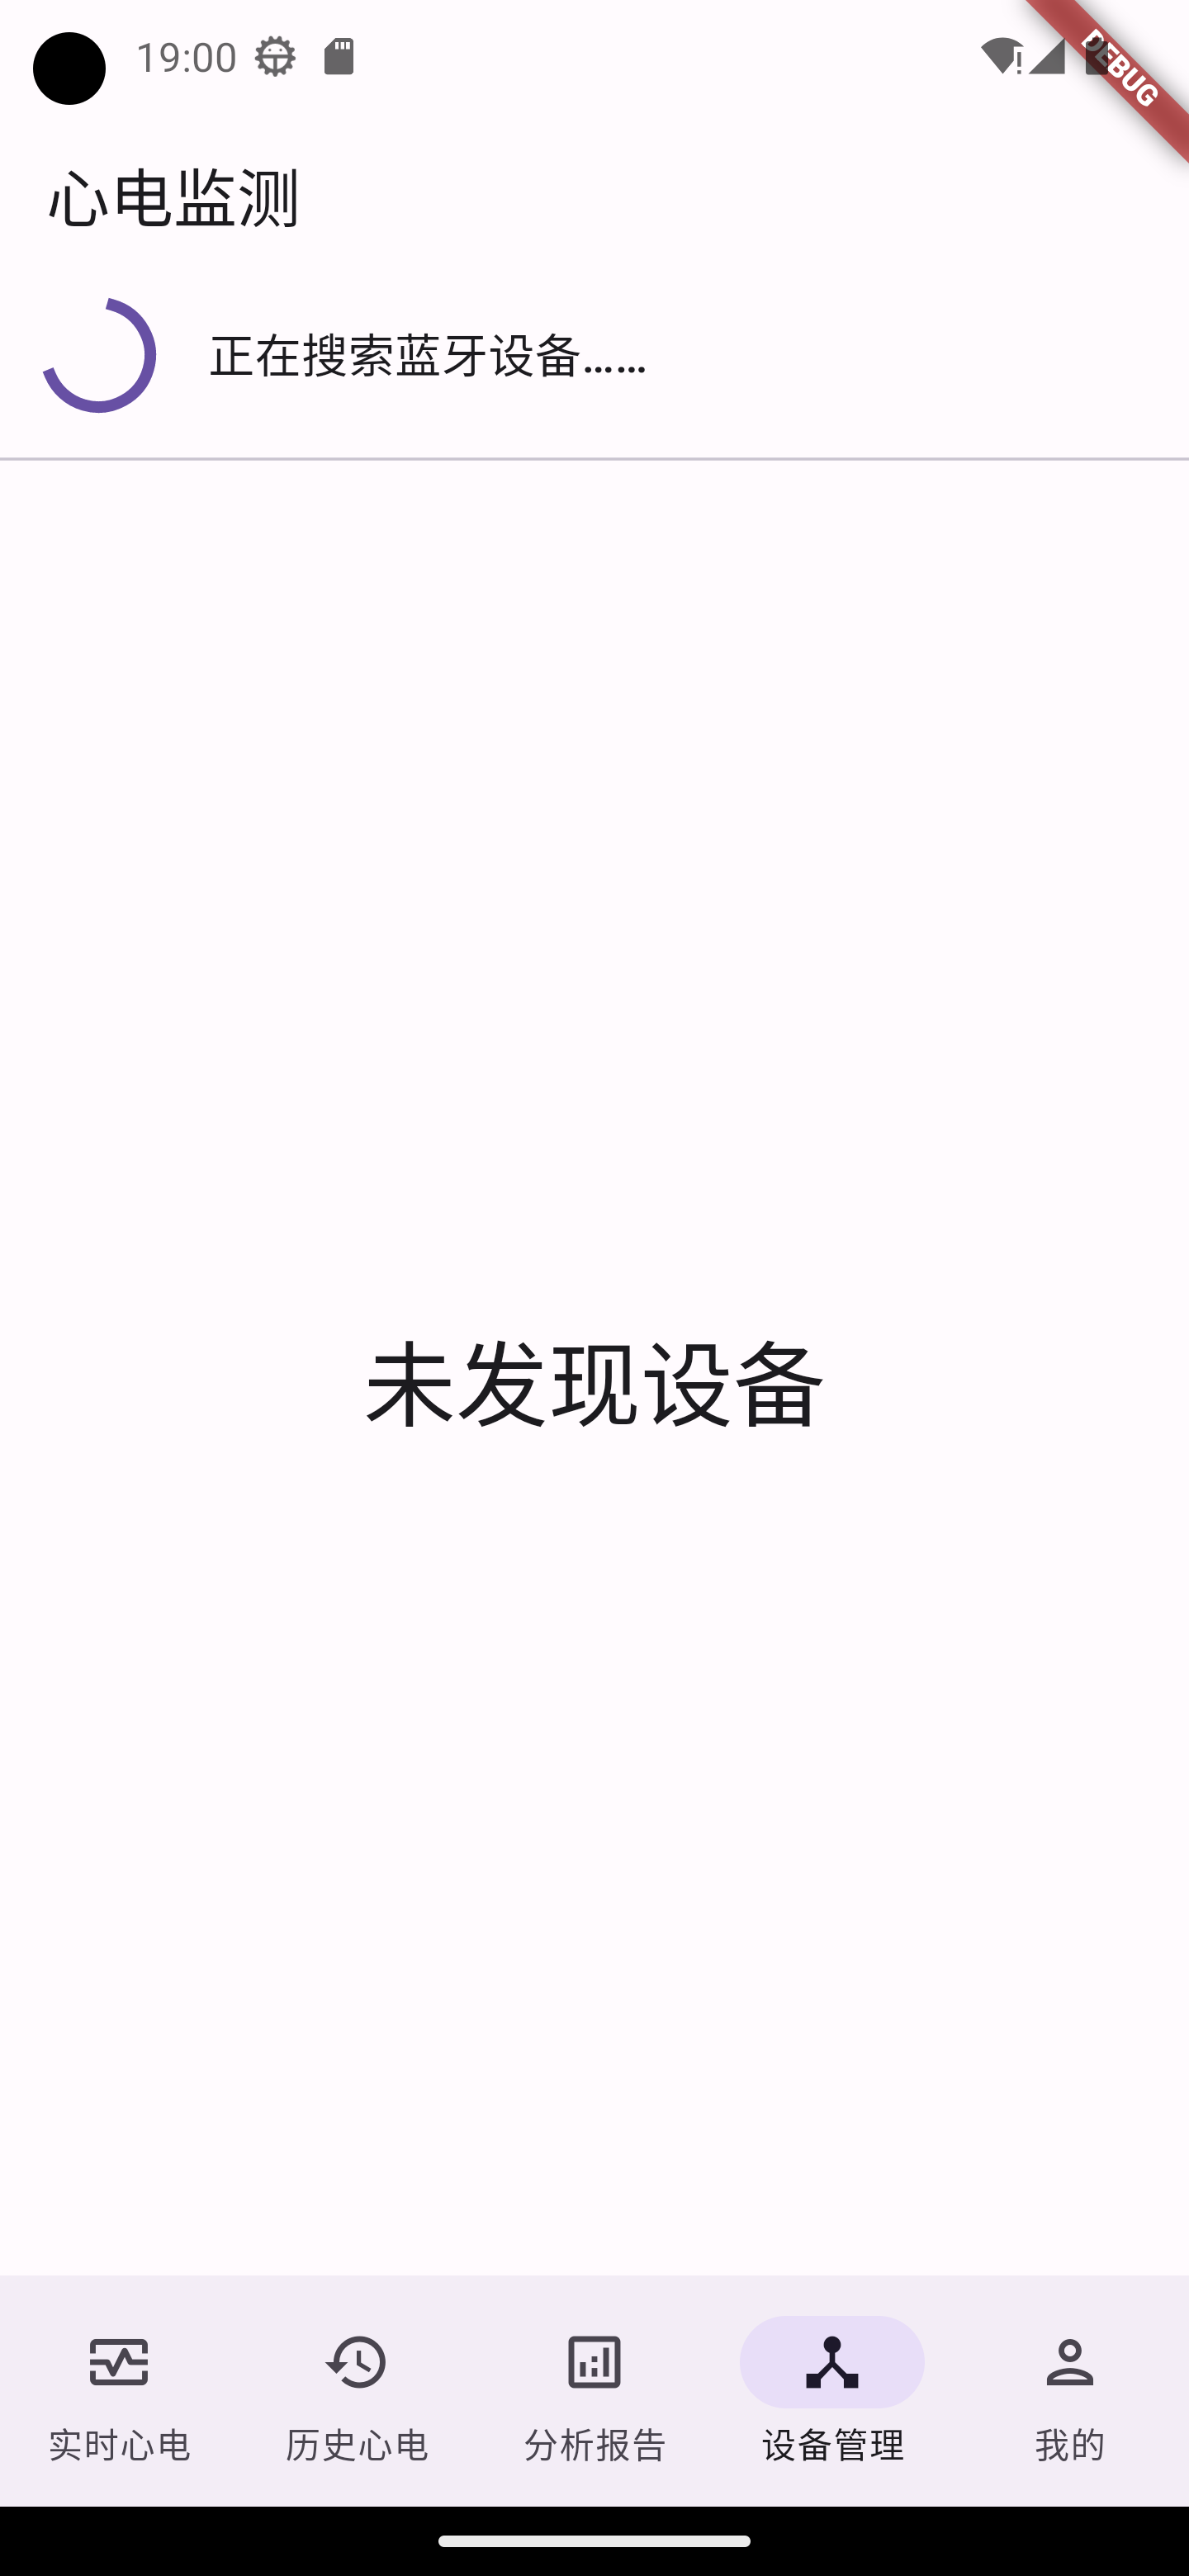
\includegraphics[width=.33\textwidth]{../assets/device-na}}
    \bicaption{设备管理界面的设计}{Design of the device page}
    \label{fig:device}
\end{figure}

\todo{设备管理界面的设计}

\subsection{其他界面的设计}\label{subsec:other-design}

应用中有一些用户不常使用,但仍然应该提供的功能,相关界面的设计如图~\ref{fig:other} 所示。

\begin{figure}[ht]
    \subcaptionbox{我的}{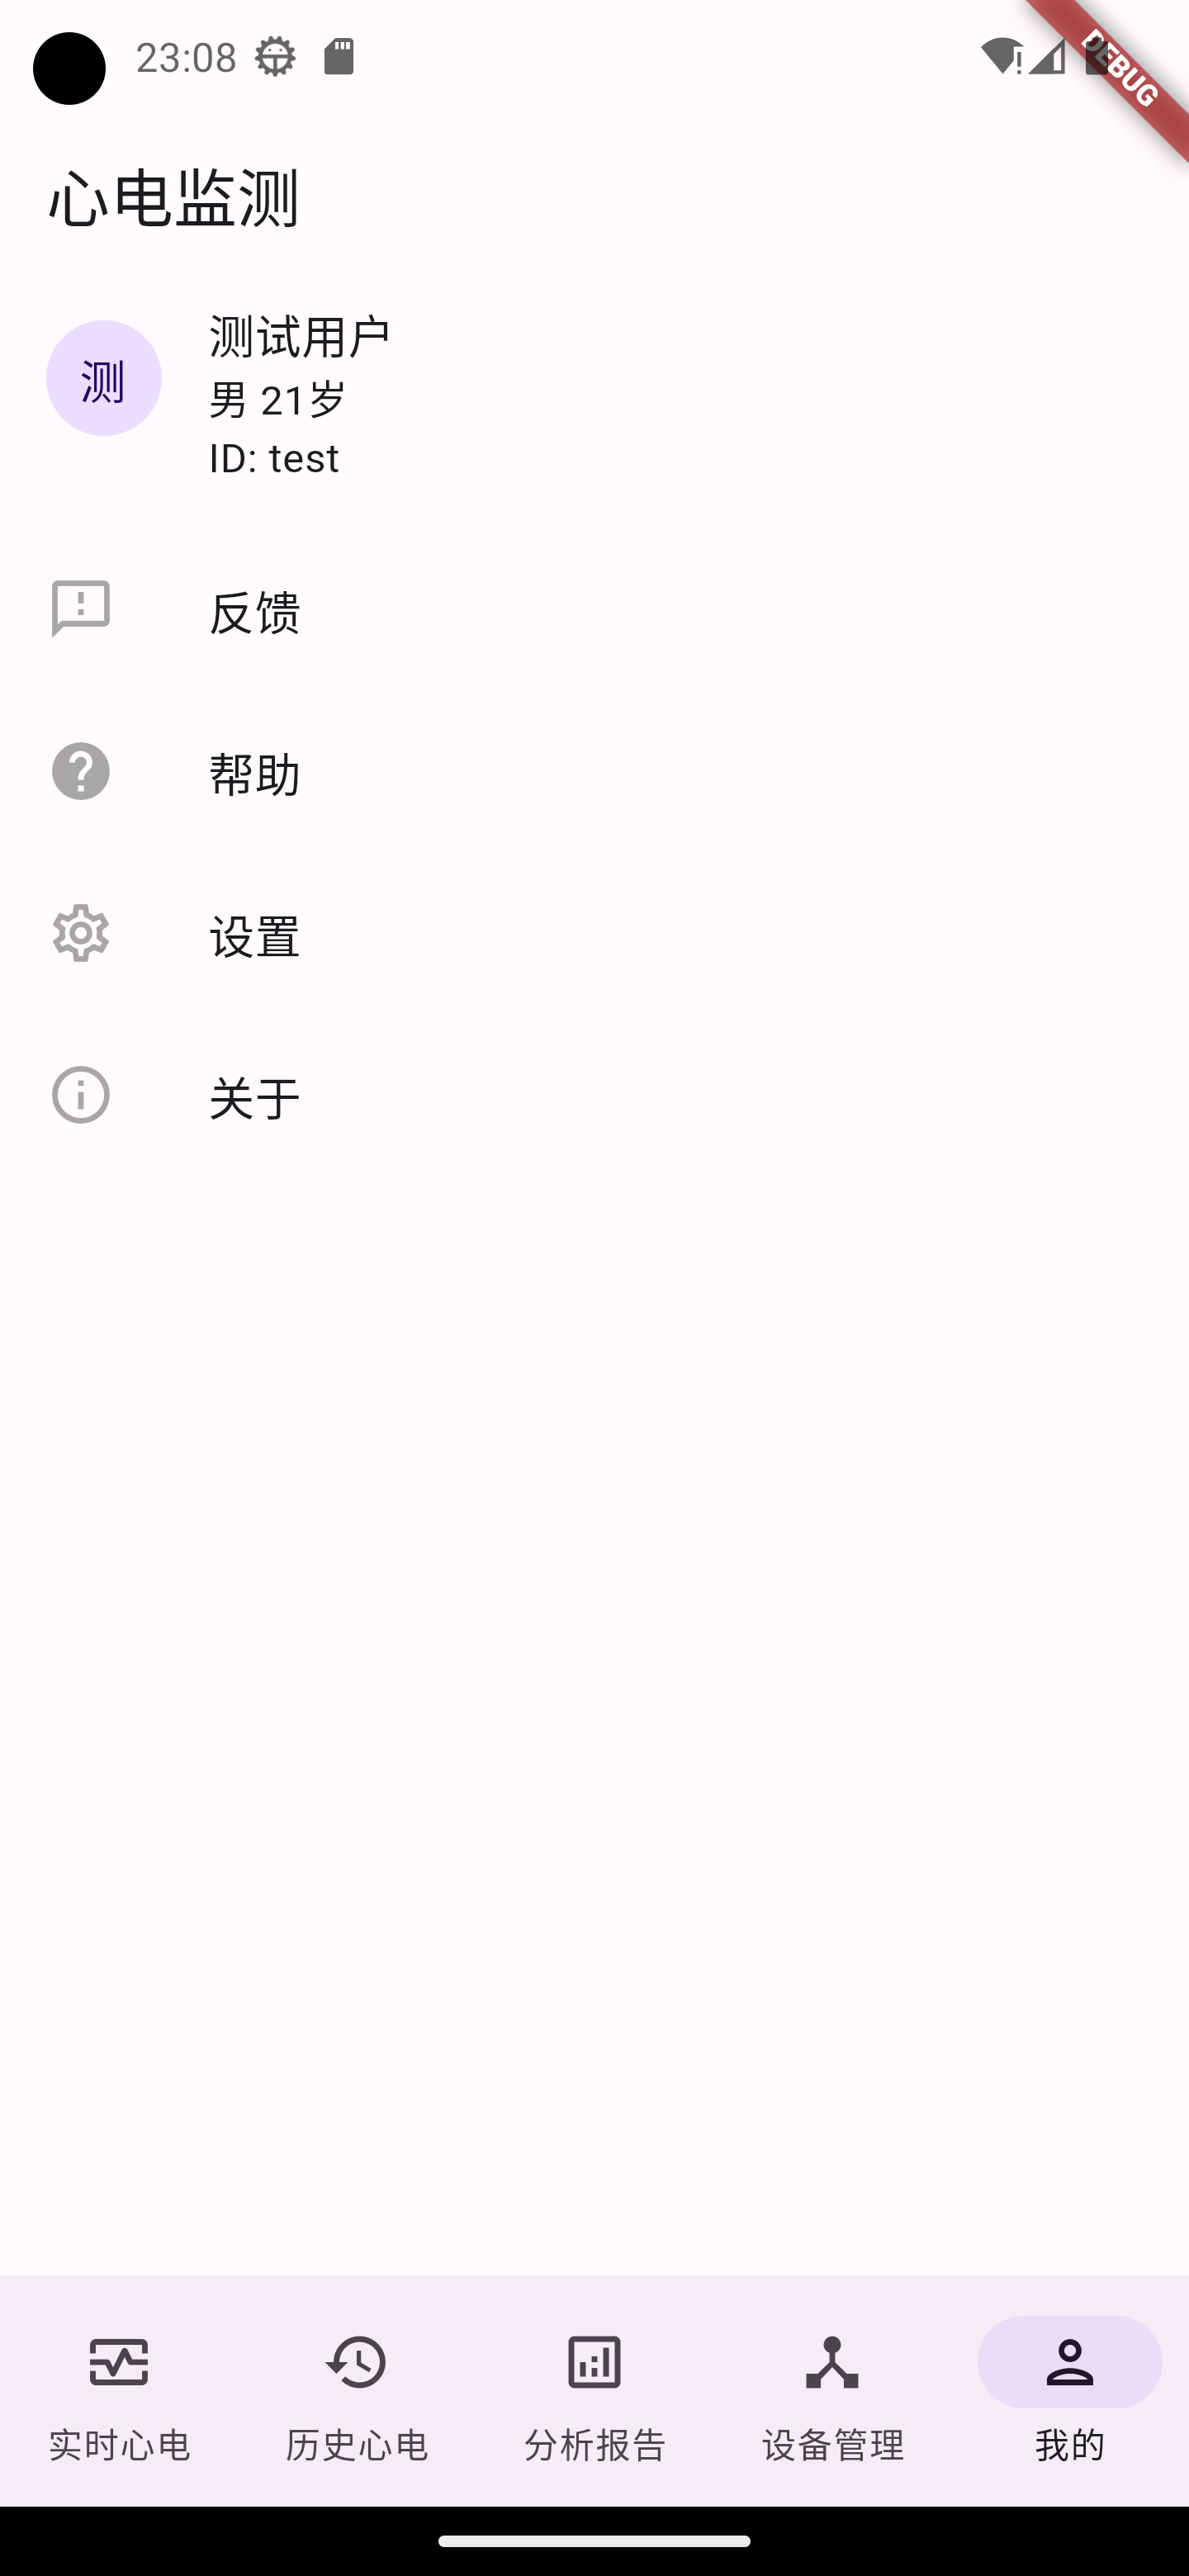
\includegraphics[width=.33\textwidth]{../assets/me}}
    \subcaptionbox{设置}{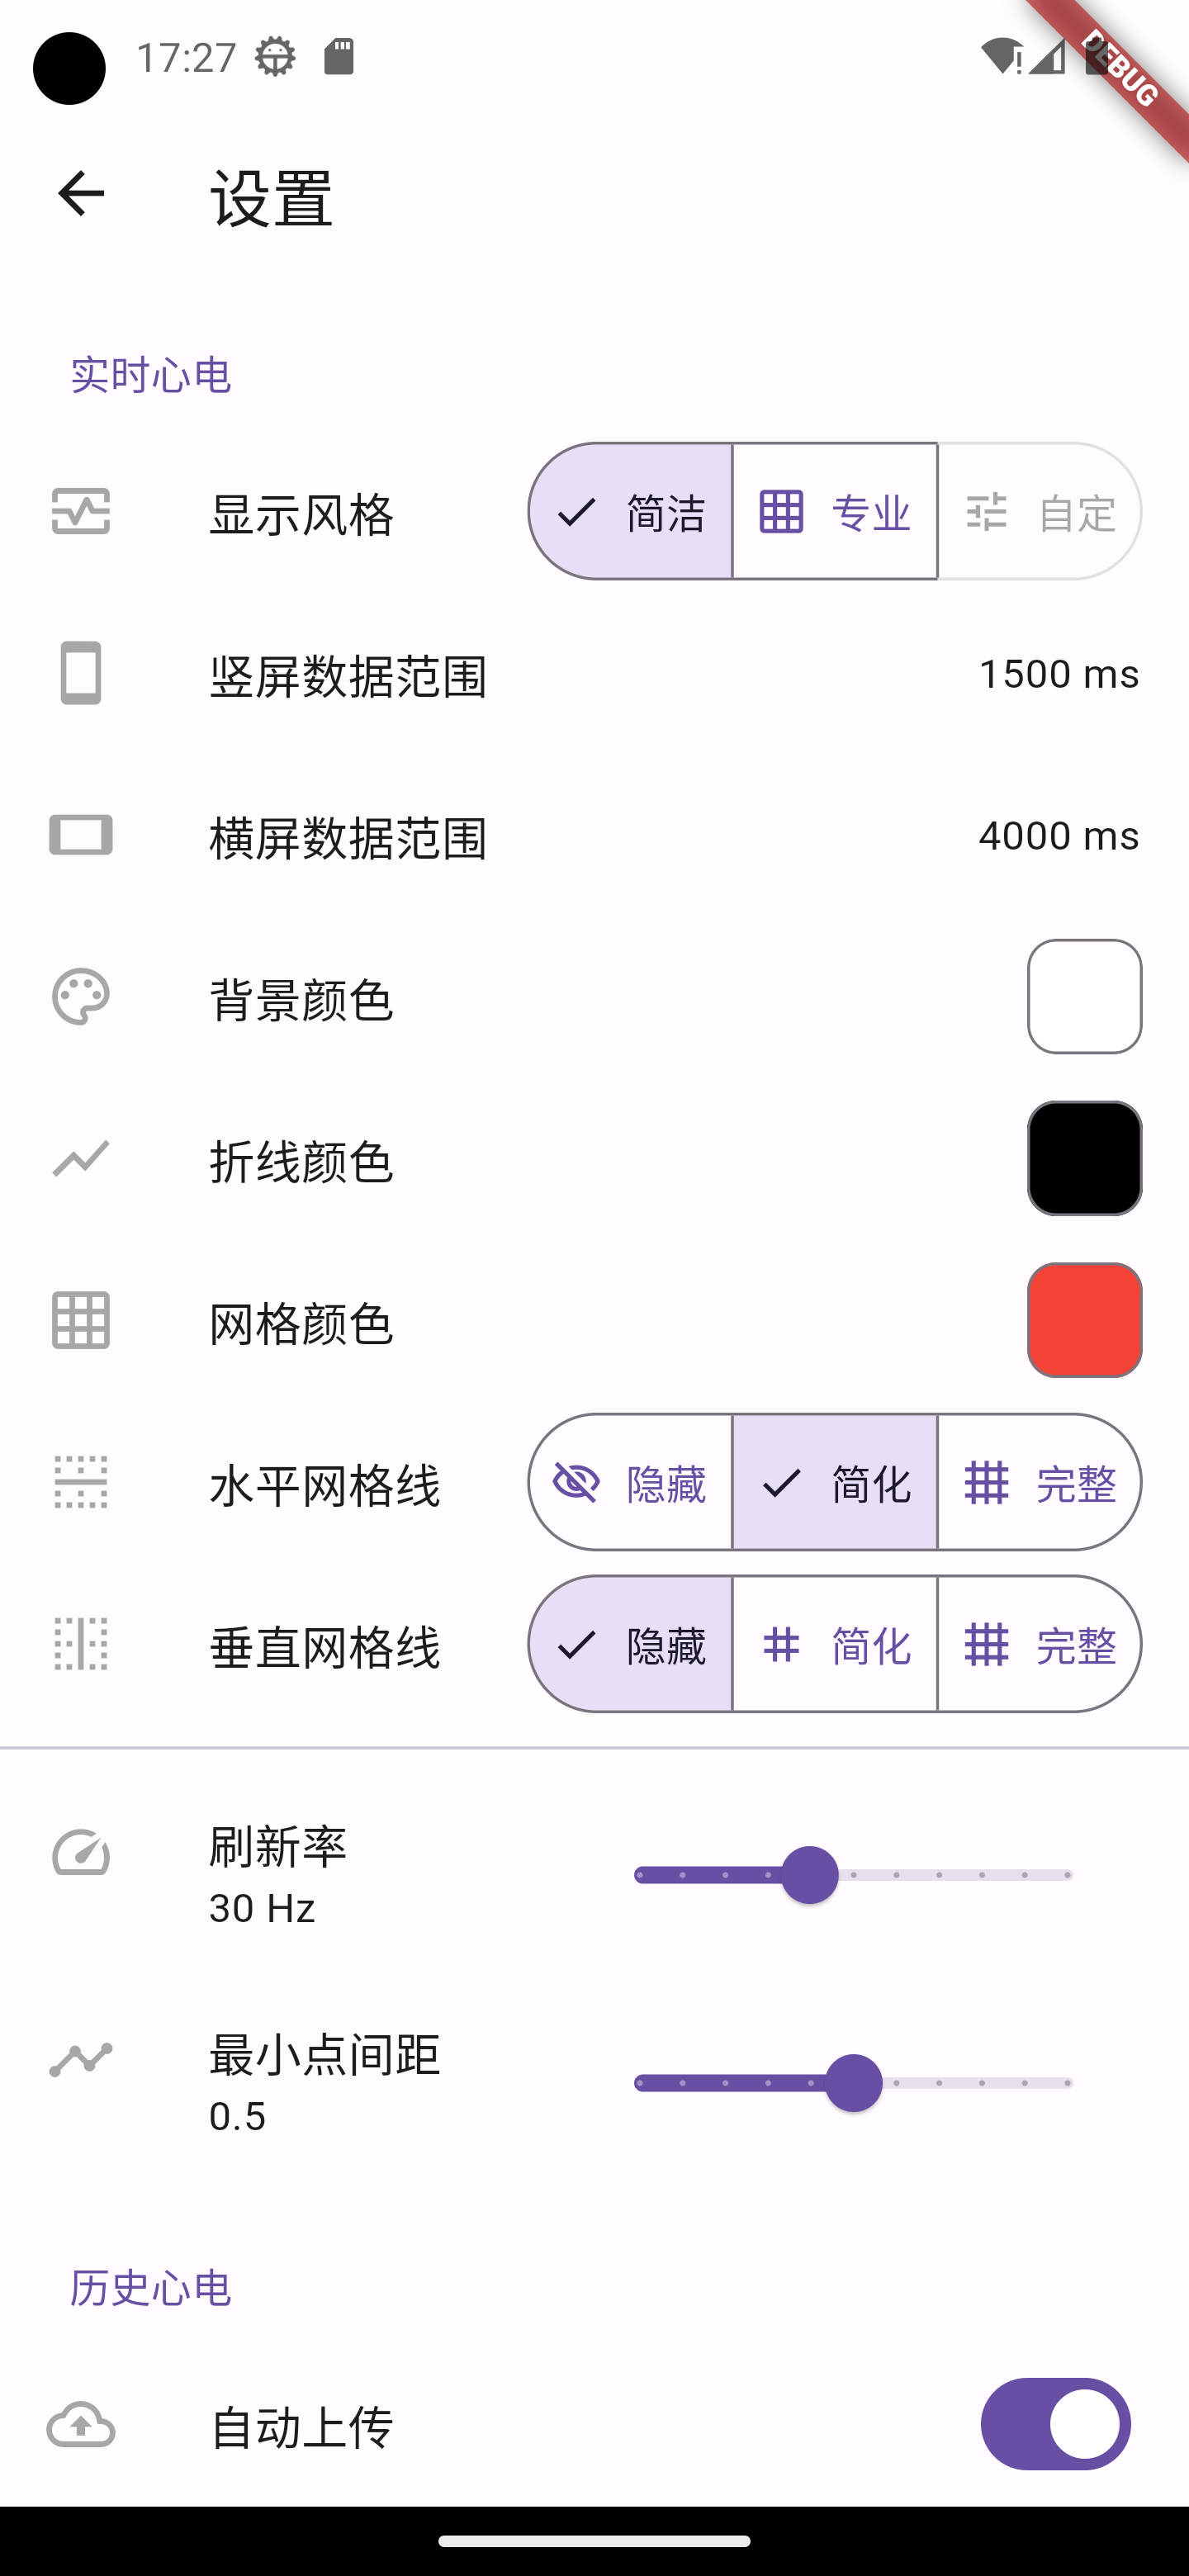
\includegraphics[width=.33\textwidth]{../assets/settings}}
    \subcaptionbox{许可}{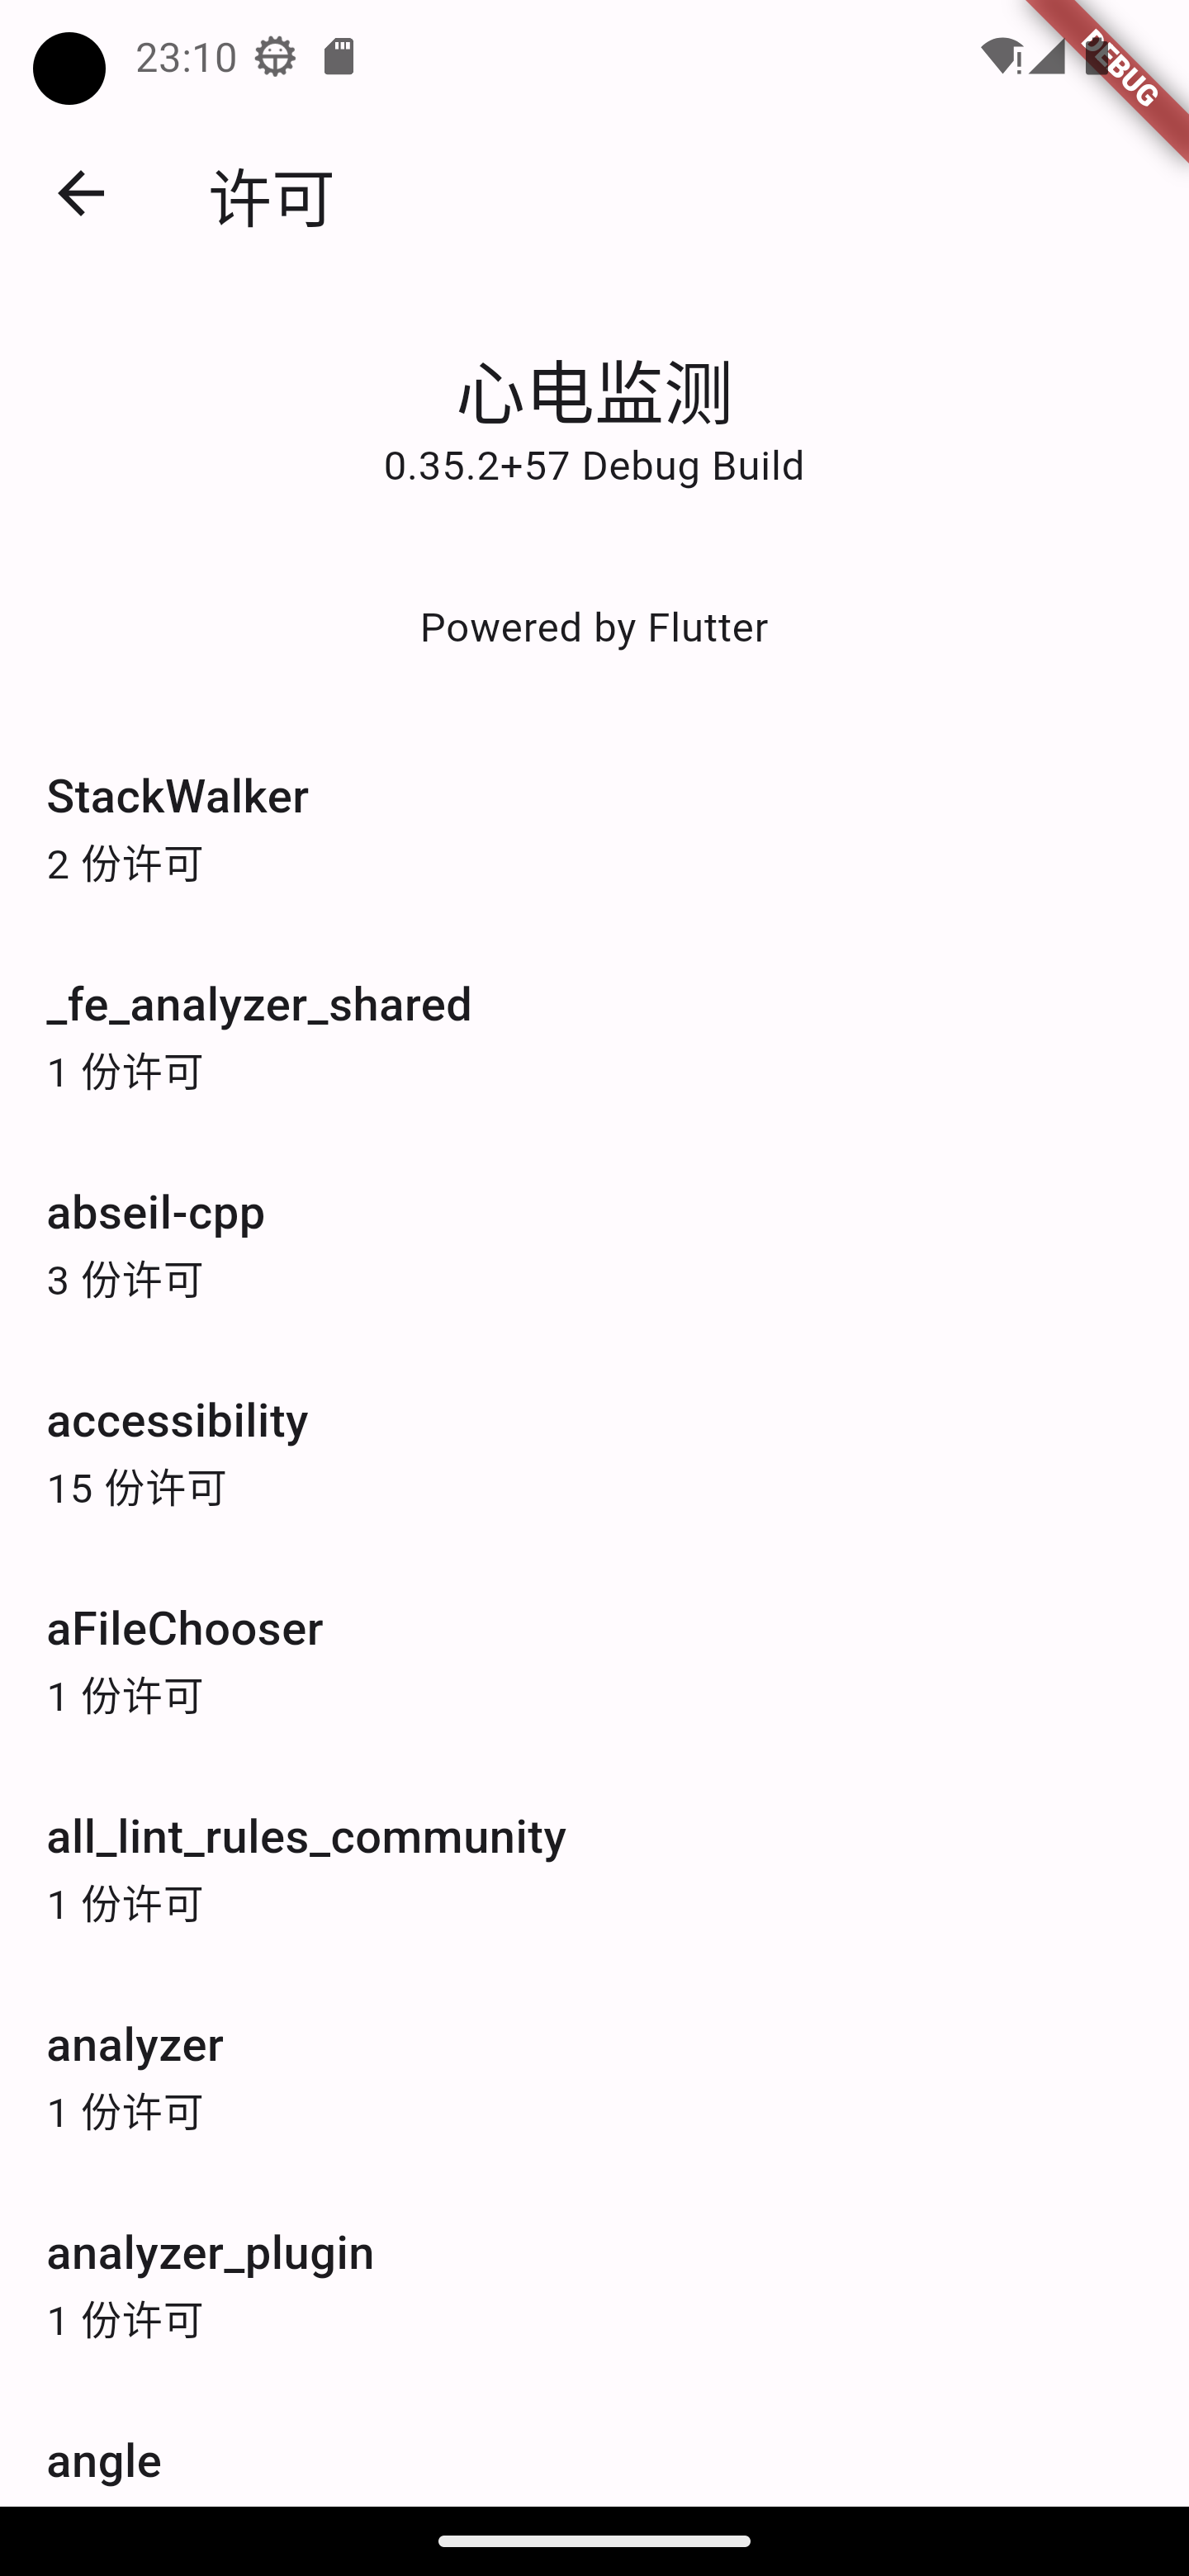
\includegraphics[width=.33\textwidth]{../assets/license}}
    \bicaption{其他界面的设计}{Design of the other pages}
    \label{fig:other}
\end{figure}

\subsubsection{我的界面的设计}\label{subsubsec:me-design}

\todo{我的界面的设计}

\subsubsection{应用设置界面的设计}\label{subsubsec:settings-design}

\todo{应用设置界面的设计}

\subsubsection{许可界面的设计}\label{subsubsec:license-design}

\todo{许可界面的设计}

\subsection{界面过渡动画的设计}\label{subsec:transition-design}

\todo{界面过渡动画的设计}

\subsection{应用的无障碍设计}\label{subsec:accessibility-design}

\todo{应用的无障碍设计}

\section{应用的数据库设计}\label{sec:db-design}

\todo{数据库设计}
